
\documentclass[UTF8,zihao=-4,oneside,openany]{ctexrep}
\usepackage[a4paper,top=2.35cm,bottom=2.45cm,left=2.35cm,right=2.35cm]{geometry}
\usepackage{fontspec}
\usepackage{xeCJK}
\setmainfont{DejaVu Sans}
\setsansfont{DejaVu Sans}
\setmonofont{Noto Sans Mono}
\setCJKmainfont{Noto Sans CJK SC}
\setCJKsansfont{Noto Sans CJK SC}
\setCJKmonofont{Noto Sans CJK SC}
\usepackage{booktabs}
\usepackage{longtable}
\usepackage{array}
\usepackage{tabularx}
\usepackage{enumitem}
\usepackage{xcolor}
\usepackage{hyperref}
\usepackage{fancyhdr}
\usepackage{titlesec}
\usepackage{lastpage}
\usepackage{pifont}
\usepackage{amsmath}
\usepackage{amssymb}
\usepackage{makecell}
\usepackage{seqsplit}
\usepackage{tikz}
\usetikzlibrary{positioning,arrows.meta,calc}
\usepackage{graphicx}
\usepackage{etoolbox}
\usepackage{caption}
\hypersetup{colorlinks=true,linkcolor=black,urlcolor=blue,citecolor=black,pdftitle={机器人示教数据质量评估框架 RDDQF v1.1 设计规范}, pdfauthor={灵机启物机器人数据质量平台}}
\definecolor{RuleBlue}{RGB}{25,74,135}
\definecolor{DeepBlue}{RGB}{17,42,86}
\definecolor{AccentBlue}{RGB}{47,105,196}
\definecolor{LightBlue}{RGB}{236,243,252}
\definecolor{LightGray}{RGB}{247,247,247}
\definecolor{LightYellow}{RGB}{255,249,230}
\definecolor{DarkGray}{RGB}{80,80,80}
\definecolor{WarnOrange}{RGB}{172,103,0}
\definecolor{RejectRed}{RGB}{150,35,35}
\definecolor{PassGreen}{RGB}{38,118,82}
\definecolor{DiagnosticPurple}{RGB}{105,72,145}
\definecolor{CoverGold}{RGB}{217,176,86}
\titleformat{\chapter}{\Huge\bfseries\color{DeepBlue}}{\thechapter}{0.9em}{}
\titleformat{\section}{\Large\bfseries\color{RuleBlue}}{\thesection}{0.8em}{}
\titleformat{\subsection}{\large\bfseries}{\thesubsection}{0.8em}{}
\titleformat{\subsubsection}{\normalsize\bfseries}{\thesubsubsection}{0.8em}{}
\titlespacing*{\chapter}{0pt}{0pt}{1.2em}
\setlist[itemize]{topsep=3pt,itemsep=2pt,parsep=0pt,leftmargin=1.9em}
\setlist[enumerate]{topsep=3pt,itemsep=2pt,parsep=0pt,leftmargin=2.2em}
\newcolumntype{Y}{>{\raggedright\arraybackslash}X}
\newcolumntype{L}[1]{>{\raggedright\arraybackslash}p{#1}}
\newcommand{\Pass}{\textcolor{PassGreen}{\ding{51}}}
\newcommand{\Warn}{\textcolor{WarnOrange}{\ding{115}}}
\newcommand{\Reject}{\textcolor{RejectRed}{\ding{55}}}
\newcommand{\Diag}{\textcolor{DiagnosticPurple}{\ding{72}}}
\newcommand{\Code}[1]{\texttt{#1}}
\newcommand{\MID}[1]{\texttt{\seqsplit{#1}}}
\newcommand{\EID}[1]{\texttt{\seqsplit{#1}}}
\newcommand{\PathNode}[1]{\textsf{#1}}
\newcommand{\Term}[1]{\textbf{#1}}
\newcommand{\docversion}{v1.1}
\newcommand{\mission}{Robot Demonstration Training Data Quality Assessment}
\newenvironment{notebox}[1]{\vspace{0.5em}\noindent\colorbox{LightBlue}{\parbox{0.96\linewidth}{\textbf{#1}}}\par\vspace{-0.2em}\begin{quote}\small}{\end{quote}\vspace{0.3em}}
\newenvironment{decisionbox}[1]{\vspace{0.5em}\noindent\colorbox{LightGray}{\parbox{0.96\linewidth}{\textbf{#1}}}\par\vspace{-0.2em}\begin{quote}\small}{\end{quote}\vspace{0.3em}}
\newenvironment{warningbox}[1]{\vspace{0.5em}\noindent\colorbox{LightYellow}{\parbox{0.96\linewidth}{\textbf{#1}}}\par\vspace{-0.2em}\begin{quote}\small}{\end{quote}\vspace{0.3em}}
\newenvironment{principlebox}[1]{\vspace{0.5em}\noindent\colorbox{LightBlue}{\parbox{0.96\linewidth}{\textbf{#1}}}\par\vspace{-0.2em}\begin{quote}\small}{\end{quote}\vspace{0.3em}}
\newenvironment{greenbox}[1]{\vspace{0.5em}\noindent\colorbox{PassGreen!10}{\parbox{0.96\linewidth}{\textbf{#1}}}\par\vspace{-0.2em}\begin{quote}\small}{\end{quote}\vspace{0.3em}}
\newenvironment{warnbox}[1]{\vspace{0.5em}\noindent\colorbox{LightYellow}{\parbox{0.96\linewidth}{\textbf{#1}}}\par\vspace{-0.2em}\begin{quote}\small}{\end{quote}\vspace{0.3em}}
\setlength{\headheight}{15pt}
\pagestyle{fancy}
\fancyhf{}
\lhead{RDDQF v1.1 设计规范}
\rhead{L3 v2 训练数据质量评估}
\cfoot{第 \thepage\ 页 / 共 \pageref{LastPage} 页}

\begin{document}


\begin{titlepage}
\thispagestyle{empty}
\begin{tikzpicture}[remember picture,overlay]
  \fill[white] (current page.south west) rectangle (current page.north east);
  \fill[DeepBlue] (current page.north west) rectangle ([xshift=3.0cm]current page.south west);
  \fill[AccentBlue] ([xshift=3.0cm]current page.north west) rectangle ([xshift=3.12cm]current page.south west);
  \fill[CoverGold] ([xshift=3.12cm,yshift=-4.2cm]current page.north west) rectangle ([xshift=3.32cm,yshift=-11.6cm]current page.north west);
  \node[rotate=90,anchor=south,white,font=\Large\bfseries] at ([xshift=1.38cm,yshift=-13.5cm]current page.north west) {RDDQF v1.1};
  \node[anchor=north east,text=DeepBlue,font=\small] at ([xshift=-1.5cm,yshift=-1.25cm]current page.north east) {正式设计规范};

  \node[anchor=north west,text=DeepBlue,text width=14.0cm,font=\Huge\bfseries] at ([xshift=4.3cm,yshift=-2.2cm]current page.north west) {机器人示教数据质量评估框架};
  \node[anchor=north west,text=DeepBlue,text width=14.0cm,font=\Large\bfseries] at ([xshift=4.3cm,yshift=-3.55cm]current page.north west) {RDDQF v1.1 设计规范};
  \node[anchor=north west,text=black,text width=14.0cm,font=\large] at ([xshift=4.3cm,yshift=-5.10cm]current page.north west) {灵机启物 L3 v2 训练数据质量评估体系};
  \node[anchor=north west,text=DarkGray,text width=14.0cm,font=\normalsize] at ([xshift=4.3cm,yshift=-5.95cm]current page.north west) {面向机器人基础模型 / 模仿学习 / VLA 数据资产治理};
  \draw[DeepBlue,line width=0.8pt] ([xshift=4.3cm,yshift=-6.80cm]current page.north west) -- ([xshift=18.1cm,yshift=-6.80cm]current page.north west);

  \node[anchor=north west,fill=LightBlue,draw=AccentBlue!35,inner sep=10pt,text width=12.9cm] at ([xshift=4.3cm,yshift=-7.35cm]current page.north west) {\small
  \textbf{文档版本：} v1.1\\[0.18cm]
  \textbf{适用范围：} L3 v2 指标引擎、证据层、报告层与前端诊断界面\\[0.18cm]
  \textbf{核心主题：} 训练数据质量评估、可解释诊断、时间完整性与相机时序连续性\\[0.18cm]
  \textbf{更新范围：} 指标修订、总分融合、Data Integrity 可靠性上限、相机同步诊断};

  \node[anchor=north west,fill=LightYellow,text=DeepBlue,inner sep=8pt,text width=12.9cm,font=\bfseries,align=center] at ([xshift=4.3cm,yshift=-12.85cm]current page.north west) {质量标准 \quad 质量本体 \quad 证据规范 \quad 指标库 \quad 引擎架构 \quad 总分融合};

  \node[anchor=north west,text=DarkGray,text width=12.9cm,font=\small] at ([xshift=4.3cm,yshift=-14.35cm]current page.north west) {本文档定义 RDDQF v1.1 的正式设计规范，用于指导 L3 v2 训练数据质量评估、证据解释、指标计算、总分融合与工程实现。};

  \node[anchor=south west,text=DeepBlue,font=\large] at ([xshift=4.3cm,yshift=1.25cm]current page.south west) {2026年6月29日};
\end{tikzpicture}
\null
\end{titlepage}



\pagenumbering{Roman}
\chapter*{文档导读与 v1.1 更新摘要}
\addcontentsline{toc}{chapter}{文档导读与 v1.1 更新摘要}
\section*{文档定位}
本文档作为 RDDQF v1.1 的正式设计总纲，覆盖训练数据质量标准、质量本体、证据规范、指标库、L3MetricsEngine v2 架构、总体架构和 v1.1 指标修订要求。

\section*{v1.1 核心设计决策}
\begin{enumerate}
\item MQ-01 评价轨迹平滑度时应使用 jerk / 加速度变化率，而不是速度变化率。
\item MQ-02 评价动作连续性时应使用 action 二阶差分，而不是 action 步长幅度。
\item MQ-03 评价动作稳定性时应关注持续震荡与手部颤振，并加入幅度门控。
\item LQ 系列指标被重新组织为有效监督覆盖率、信息强度和低价值持续片段占比。
\item DI-01 / DI-02 从简单 CV 和固定阈值检查升级为鲁棒时间完整性诊断。
\item DX-01 仅作为执行链路诊断，不进入训练质量总分。
\item Data Integrity 既参与评分，也作为训练质量总分的可靠性上限条件。
\item 腕部相机卡顿、冻结帧和传感器级同步错位被纳入 Camera Temporal Continuity 证据体系。
\end{enumerate}

\tableofcontents
\clearpage
\pagenumbering{arabic}
\chapter{训练数据质量标准}

\section{背景与问题定义}

\subsection{从运动质检到训练数据质检}

在机器人数据采集平台中，质量检查通常容易从机器人控制视角出发：轨迹是否平滑、关节是否跟踪目标、执行力矩是否过大、时间戳是否稳定。这些指标对机器人系统调试非常有价值，但它们不一定等价于训练数据质量。

对于下游策略学习而言，一条 episode 的价值不主要取决于机器人控制器是否完美执行每个目标关节位置，而取决于这条 demonstration 是否向模型提供了清晰、稳定、可学习的“观测到动作”的映射。模型最终学习的是在给定任务语义、视觉观测和机器人状态的条件下，应该输出什么动作。因此，L3 需要回答的问题应从：

\begin{quote}
机器人这次执行得好不好？
\end{quote}

转变为：

\begin{quote}
这条 demonstration 是否值得作为训练样本进入数据集？
\end{quote}

这两个问题看似接近，但会导致完全不同的指标体系。例如，\texttt{actions} 与 \texttt{qpos} 的差值能够反映控制器命令跟踪情况，却不必然反映该 demonstration 是否可用于训练；而动作抖动、无意义停顿、关键动作缺失、任务失败、观测不可用等问题，反而会直接影响模型学习。

\subsection{当前 L3 v1 的主要错位}

当前 L3 v1 具有工程上合理的一面：它基于 \texttt{telemetry.npz} 中的时序数据自动计算，能够在人工 QC 页面展示综合分、子指标和异常时间段。但从训练数据筛选的角度看，存在如下目标错位：

\begin{enumerate}
  \item \textbf{评价对象偏向机器人执行，而非 demonstration。} 例如 Tracking Error 更多评价控制器是否忠实执行目标命令，而不是数据本身是否对模型有学习价值。
  \item \textbf{指标聚合偏向运动学异常，而非训练有效性。} 平滑度、饱和、停滞等指标被直接合成为 \texttt{Q\_motion}，但缺乏“是否影响模型学习”的中间解释。
  \item \textbf{缺少任务语义。} 同样的动作停顿、手部 0 或 255、末端轨迹绕行，在不同任务中可能含义完全不同。
  \item \textbf{缺少数据集视角。} 单条 episode 的指标无法回答它在同类任务中的相对质量、重复性、覆盖度和多样性。
  \item \textbf{缺少训练格式意识。} 未来训练样本通常以 observation-state-action-task 的形式组织，而现有 L3 没有明确区分 observation 质量、action 标签质量和 state-action 一致性。
\end{enumerate}

因此，L3 v2 不应只是对 L3 v1 的局部阈值调整，而应以“训练数据质量”为目标重新定义标准。

\subsection{本文档的目标}

本文档定义 L3 v2 的上层质量标准，具体目标包括：

\begin{itemize}
  \item 明确 L3 v2 的评价对象是 robot demonstration，而非机器人控制器。
  \item 明确训练数据质量的核心标准是 learnability，即样本是否能为下游策略学习提供有效学习信号。
  \item 将 episode 级质量拆解为若干一级维度，为后续指标设计提供稳定框架。
  \item 明确哪些指标应作为核心训练质量指标，哪些只能作为辅助诊断指标。
  \item 明确 L3 与 L2、L4、批次报告和未来数据资产平台之间的关系。
\end{itemize}

\section{适用范围与非目标}

\subsection{适用范围}

本文档适用于以下数据与流程：

\begin{itemize}
  \item 由 TeleDex 系统采集并转换得到的 processed episode。
  \item 包含多路 RGB/Depth 视频、时间戳、机器人关节状态、遥操作目标动作、力信息、同步校验、末端位姿、IMU 或触觉等字段的数据。
  \item 用于具身智能模型、机器人模仿学习模型、VLA 模型或行为克隆模型训练的数据筛选流程。
  \item L3 自动质检、人工 QC 工作台、批次报告、数据集构建和数据资产分层。
\end{itemize}

\subsection{非目标}

本文档明确不解决以下问题：

\begin{itemize}
  \item 不评价机器人硬件是否健康。
  \item 不评价底层控制器是否达到最佳跟踪性能。
  \item 不替代 L4 对任务完成度的人工判断。
  \item 不替代 L2 对视觉质量的人工或自动判断。
  \item 不直接规定所有指标的最终公式和阈值。
  \item 不判断某个具体模型架构应该如何使用数据。
\end{itemize}

这些内容可以在后续的《L3 v2 指标设计规范》《批次级数据集质量报告规范》和《模型训练数据导出规范》中进一步展开。

\section{核心定义}

\subsection{Episode}

Episode 指一次完整的机器人遥操作采集片段。它通常对应 processed 目录下的一个 \texttt{episode\_XXXXXX}，包含统一时间轴上的视频、机器人状态、遥操作动作、同步信息和元数据。Episode 是 L3 自动质检的基本单位。

\subsection{Demonstration}

Demonstration 指在特定任务提示、场景状态和机器人初始状态下，由操作者通过遥操作设备产生的一段可供模型模仿学习的行为示范。它不仅包括动作序列，还包括动作发生时的视觉观测、机器人状态、任务语义和最终任务结果。

本文档中的 demonstration 不是“机器人机械运动轨迹”的同义词。它是一个训练样本级对象，包含以下组成部分：

\begin{itemize}
  \item 任务语义：如抓取、放置、倾倒、移动、整理等。
  \item 观测输入：RGB、Depth、机器人状态、可能的触觉或 IMU。
  \item 动作标签：遥操作设备发出的目标关节位置，通常对应 \texttt{actions}。
  \item 状态反馈：机器人实际关节位置、速度、力等，通常对应 \texttt{qpos}, \texttt{qvel}, \texttt{effort}。
  \item 结果信息：任务是否完成，是否碰撞，是否失败，是否需要人工复核。
\end{itemize}

\subsection{Observation}

Observation 指模型在某个时刻可见的输入信息，包括多路相机图像、深度图、机器人当前状态、任务提示以及可选传感器信息。Observation 的质量决定模型是否能从场景中理解任务状态。

\subsection{Action}

Action 指模型需要学习预测的动作标签。在当前 TeleDex 数据语义下，\texttt{actions} 来自遥操作设备发送的控制命令，通常是目标关节位置。机械臂动作以弧度表示，灵巧手动作为 0 至 255 范围值。

因此，\texttt{actions} 在训练数据中更接近“人类操作者意图的标签”，而不是机器人实际执行结果。

\subsection{State}

State 指机器人当前实际状态，主要包括 \texttt{qpos}, \texttt{qvel}, \texttt{effort} 和可能的末端位姿。State 可以作为训练输入的一部分，也可以用于检查动作标签和环境变化之间是否存在明显矛盾。

\subsection{Training Data Quality}

Training Data Quality 指一条 demonstration 对下游策略学习的有效性、清晰性、稳定性和可复用价值。它不是控制精度的同义词，也不是任务成功的单一标签，而是一个综合属性。

本文档采用如下定义：

\begin{quote}
一条高质量机器人训练数据，是指在任务语义明确、观测可用、动作标签有效、状态演化合理、任务过程完整且无严重噪声污染的条件下，能够为下游策略模型提供稳定、清晰、可学习行为信号的 demonstration。
\end{quote}

\section{L3 v2 的 Mission Statement}

\begin{principlebox}{Mission Statement}
L3 的目标不是评价机器人执行得有多好，而是评价这条 demonstration 对下游策略学习有多大的训练价值。
\end{principlebox}

该 mission statement 是后续所有指标取舍的最高原则。任何拟进入 L3 v2 的指标，都必须回答至少一个问题：

\begin{itemize}
  \item 它是否影响 observation 到 action 的学习？
  \item 它是否影响动作标签的可靠性？
  \item 它是否影响任务语义与行为之间的一致性？
  \item 它是否影响数据导出后的训练稳定性？
  \item 它是否能帮助人工快速判断该样本是否应进入训练集？
\end{itemize}

如果一个指标只能评价机器人硬件或控制器，而不能解释它如何影响训练数据质量，则该指标不应作为核心 L3 训练质量指标。它可以保留为辅助诊断信息，但不应主导总分。

\section{质量哲学与设计原则}

\subsection{原则一：质量由可学习性定义，而非执行精度定义}

\begin{principlebox}{Principle 1: Learnability over execution accuracy}
训练数据质量的核心是模型是否能从样本中学习到清晰、稳定、可泛化的行为模式，而不是机器人是否以最小误差跟踪了每个目标关节命令。
\end{principlebox}

这意味着 Tracking Error 不应天然成为核心质量指标。若一条 demonstration 的动作标签清晰、过程流畅、任务成功、观测完整，即使存在一定控制跟踪误差，它仍可能是高价值训练数据。相反，如果机器人跟踪误差很小，但操作者动作混乱、重复修正、任务失败、视频遮挡严重，这条数据也不应被认为高质量。

\subsection{原则二：评价对象是 demonstration，而不是机器人}

\begin{principlebox}{Principle 2: Demonstration-centric evaluation}
L3 v2 评价的是一次示范是否适合被模型模仿，而不是机器人平台、控制器、伺服系统或硬件状态是否优秀。
\end{principlebox}

这一区分对指标设计非常关键。控制器诊断类信息可以帮助定位采集现场问题，但不应与训练质量混为一谈。L3 v2 应优先关注动作标签、观测、状态演化和任务过程是否构成一条可学习 demonstration。

\subsection{原则三：评价信息价值，而不是单纯物理量}

\begin{principlebox}{Principle 3: Information value over raw physical magnitude}
对训练数据而言，关键不是某个物理量大不大，而是它是否改变了样本的信息含量、标签可靠性或学习信号质量。
\end{principlebox}

例如，长时间静止不一定是坏的。如果静止发生在任务开始前或完成后，它可以被裁剪；如果静止发生在等待物体稳定的任务阶段，它可能是合理的；如果静止发生在关键操作过程中并伴随动作缺失，则会降低训练价值。因此，指标必须结合时间阶段和任务语义解释。

\subsection{原则四：动作标签是训练核心，不是附属诊断量}

\begin{principlebox}{Principle 4: Action labels are first-class training signals}
\texttt{actions} 是模型未来需要学习预测的标签，应被视为训练数据的核心组成部分，而不是仅用于与 \texttt{qpos} 做差的诊断变量。
\end{principlebox}

这意味着 L3 v2 应重点评价 \texttt{actions} 是否可学习：是否连续、是否稳定、是否存在高频抖动、是否长时间无信息、是否出现非人类操作模式、是否与任务阶段相匹配。

\subsection{原则五：任务上下文优先于统一阈值}

\begin{principlebox}{Principle 5: Task-aware quality interpretation}
同一数值异常在不同任务中可能有不同含义。L3 v2 应逐步从全局阈值转向任务类型感知和同类任务分布对比。
\end{principlebox}

例如，灵巧手动作接近 0 或 255，在某些任务中可能代表合法的完全张开或完全闭合；在另一些任务中，快速反复接近两端则可能代表标签抖动。L3 v2 不应简单把边界值判为饱和异常，而应判断其是否构成不合理的动作模式。

\subsection{原则六：单条质量与批次价值分离}

\begin{principlebox}{Principle 6: Episode quality and dataset value are related but not identical}
单条 episode 的训练质量与整个数据集的覆盖度、多样性和均衡性不同。L3 主要评价单条 demonstration，批次报告应进一步评价数据集层面的价值。
\end{principlebox}

一条动作标准但非常重复的 episode 可能单条质量合格，但对扩展数据集覆盖度的边际价值较低。这类判断不适合完全放入 L3 单条总分，应进入批次级数据资产报告。

\section{高质量训练数据的标准定义}

\subsection{一句话定义}

高质量机器人训练数据应满足：任务语义明确、观测可用、动作标签有效、状态变化合理、过程连贯、关键动作充分、任务结果可信，并能够为模型提供清晰稳定的 observation-state-action 学习信号。

\subsection{必要条件}

一条 demonstration 至少应满足以下必要条件，才可进入训练候选集：

\begin{enumerate}
  \item \textbf{数据结构完整。} 必需文件存在，关键字段可读取，时间轴长度一致或可对齐。
  \item \textbf{观测可用。} 至少主视角视频可用，关键操作阶段无遮挡、不过曝、不严重模糊。
  \item \textbf{动作标签存在且有效。} \texttt{actions} 不应为空、不应全零、不应大面积无效。
  \item \textbf{时间顺序正确。} 时间戳应单调，帧率和同步误差应在训练可接受范围内。
  \item \textbf{任务过程可解释。} 数据应包含与任务提示一致的操作过程，而不是无关动作或错误任务。
  \item \textbf{任务结果可信。} 至少应能通过 L4 或后续结果标签判断任务是否完成。
\end{enumerate}

\subsection{优秀条件}

在满足必要条件后，一条优秀 demonstration 应进一步具备：

\begin{itemize}
  \item 动作自然、连续、平滑，没有大量犹豫和重复修正。
  \item 关键动作阶段清晰，例如接近、接触、抓取、移动、释放等阶段可被视觉和状态共同解释。
  \item 动作标签具有足够信息密度，不是长时间无意义静止或重复无效小动作。
  \item 轨迹相对高效，不存在明显绕远、反复试探或无关操作。
  \item 同类任务中具有代表性，既不过于异常，也能补充数据集覆盖。
\end{itemize}

\subsection{不合格条件}

出现以下情况时，该 demonstration 应被拒绝进入训练集，或至少进入人工复核：

\begin{itemize}
  \item 任务明显失败，且失败原因不作为专门失败数据集使用。
  \item 关键观察视角不可用，无法看清关键物体或机器人交互。
  \item 动作标签严重抖动、跳变、缺失或与任务无关。
  \item 时间戳错乱、同步严重异常、视频与遥测明显错位。
  \item 采集开始或结束裁剪错误，导致缺少关键任务阶段。
  \item 数据字段语义不一致，例如 \texttt{actions} 维度错位、手臂和手部单位混淆。
\end{itemize}

\section{质量维度体系}

L3 v2 应将训练数据质量拆解为九个维度。每个维度都回答一个不同的问题。

\begin{longtable}{p{0.18\linewidth}p{0.32\linewidth}p{0.38\linewidth}}
\toprule
\textbf{质量维度} & \textbf{核心问题} & \textbf{主要关注对象} \\
\midrule
D1 数据完整性 & 数据能否被稳定读取和导出？ & 文件、字段、维度、帧数、元数据 \\
D2 时间一致性 & 时序是否可信？ & timestamps、fps、同步误差、缺帧 \\
D3 观测可用性 & 模型能否看清任务状态？ & RGB、Depth、多视角、L2 结果 \\
D4 动作标签质量 & action 是否适合作为训练标签？ & actions 连续性、抖动、有效性 \\
D5 状态动作一致性 & 动作与状态变化是否相互解释？ & qpos、qvel、actions、ee pose \\
D6 示范过程质量 & 操作者示范是否自然高效？ & 停顿、犹豫、重复修正、轨迹效率 \\
D7 任务语义一致性 & 行为是否符合 task prompt？ & 任务类型、动作阶段、结果标签 \\
D8 任务结果质量 & 任务是否完成且结果可信？ & L4 pass/fail、人工备注、终态 \\
D9 数据集价值 & 该样本对整体数据集是否有贡献？ & 同类分布、代表性、多样性、稀缺性 \\
\bottomrule
\end{longtable}

这九个维度并不都适合由 L3 完全自动判定。其中 D1、D2、D4、D5、D6 更适合 L3 自动计算；D3 与 L2 强相关；D8 与 L4 强相关；D7 需要任务类型与人工标签逐步增强；D9 更适合批次级或数据集级报告。

\section{维度 D1：数据完整性}

\subsection{定义}

数据完整性评价 episode 是否具备进入训练流水线的基本结构条件。它回答的问题是：数据是否能被稳定读取、解析、对齐和导出。

\subsection{基本要求}

\begin{itemize}
  \item processed 目录存在，且包含 \texttt{telemetry.npz}, \texttt{manifest.json}, \texttt{metadata.json}, \texttt{camera\_info.json} 等核心文件。
  \item 至少一条可用于训练的 RGB 视频存在，且与时间戳文件长度一致。
  \item \texttt{telemetry.npz} 至少包含 \texttt{timestamps}, \texttt{qpos}, \texttt{actions}。
  \item 关键数组的第一维长度一致，或可以明确映射到统一时间轴。
  \item 机器人自由度维度可解释，不存在无法识别的维度错位。
\end{itemize}

\subsection{质量解释}

数据完整性是硬性前置条件。若数据结构无法稳定读取，则后续再好的动作或任务表现都无法进入训练流水线。D1 的结果应更多表现为 gate，而不是连续分数。

\section{维度 D2：时间一致性}

\subsection{定义}

时间一致性评价视频、状态、动作和传感器数据是否在统一时间轴上可信。它是训练数据可用性的底层保障。

\subsection{与训练的关系}

策略学习依赖 observation 与 action 的正确配对。如果视频帧对应的是 $t$ 时刻，而 action 实际来自 $t+\Delta t$，模型将学习到错误的因果关系。同步错误的危害通常比轻微轨迹不平滑更大，因为它直接污染监督信号。

\subsection{应关注的问题}

\begin{itemize}
  \item 时间戳是否单调递增。
  \item 帧间隔是否稳定，是否存在异常跳变。
  \item \texttt{sync\_validation\_is\_valid} 是否大面积失败。
  \item \texttt{sync\_validation\_max\_diff} 是否在关键动作阶段过大。
  \item metadata 中记录的对齐方式、裁剪范围和最大时间差是否合理。
\end{itemize}

\subsection{对现有指标的影响}

当前 Timestamp Jitter 和同步异常 timeline 应保留，并从“运动质量指标”改归为“时间一致性指标”。它们应具备较高优先级，因为时序错位会直接影响 observation-action 训练配对。

\section{维度 D3：观测可用性}

\subsection{定义}

观测可用性评价模型输入是否能支持任务理解。它包括视觉清晰度、视角覆盖、关键物体可见性、深度可用性和多模态一致性。

\subsection{与 L2 的关系}

当前体系中 L2 已经负责视觉质量人工判断，包括模糊、过曝、遮挡、深度异常等问题。因此，L3 v2 不应重复实现完整视觉质检，但应接入 L2 结果作为训练质量的一部分。

\subsection{L3 应如何使用 D3}

L3 v2 可在以下层面使用观测信息：

\begin{itemize}
  \item 将 L2 视觉质量结论作为训练质量总判断的强约束。
  \item 在 timeline 中将关键动作阶段与视觉异常段对齐展示。
  \item 在未来引入“关键交互阶段可见性”指标，例如抓取瞬间手和物体是否可见。
  \item 对 RGB、Depth、状态曲线和动作曲线进行联合复核，而不是孤立展示运动指标。
\end{itemize}

\section{维度 D4：动作标签质量}

\subsection{定义}

动作标签质量是 L3 v2 的核心维度之一。它评价 \texttt{actions} 是否适合作为模型训练标签。

\subsection{为什么 action 质量比 tracking error 更关键}

在模仿学习或 VLA 训练中，模型通常学习从 observation 和 state 到 action 的映射。因此，\texttt{actions} 是监督标签。如果标签本身抖动、跳变、失真或长时间无意义，模型会直接学习到这些缺陷。

相比之下，\texttt{qpos} 与 \texttt{actions} 的差值更多反映控制器执行和机器人动态响应。它可以辅助判断状态动作一致性，但不应替代对 action 标签自身质量的评价。

\subsection{高质量 action 的特征}

\begin{itemize}
  \item 连续：相邻动作之间变化合理，不出现非物理跳变。
  \item 稳定：不存在高频抖动或方向频繁翻转。
  \item 有效：在关键任务阶段包含足够动作信息，而非长期静止或全零。
  \item 可解释：动作变化能与视觉和状态变化对应。
  \item 单位一致：机械臂与灵巧手维度单位正确，归一化方式明确。
\end{itemize}

\subsection{对现有指标的影响}

\begin{itemize}
  \item Dead Actions 应从“无效动作占比”重命名为“动作信息缺失”或“动作低信息段”。它不应简单惩罚所有静止，而应结合任务阶段和裁剪边界解释。
  \item Saturation 不应简单认为手部 0 或 255 是坏数据。更合理的判断是：是否存在长期卡边界且无状态变化，或高频在边界之间跳变。
  \item Chatter 应提升为核心动作标签质量指标，尤其对灵巧手训练非常重要。
  \item LDLJ 若继续使用，应更多关注 action 的平滑性和末端动作平滑性，而不是只评价 arm 的 qpos。
\end{itemize}

\section{维度 D5：状态动作一致性}

\subsection{定义}

状态动作一致性评价动作标签、机器人状态和场景变化之间是否存在明显矛盾。它不是要求 \texttt{qpos} 精确等于 \texttt{actions}，而是要求它们在训练意义上相互可解释。

\subsection{Tracking Error 的重新定位}

当前 Tracking Error 计算 \texttt{|actions - qpos|} 的 P95，并按 arm 和 hand 加权。该指标的物理意义明确，但它更接近命令执行误差或控制器跟踪误差。

在 L3 v2 中，Tracking Error 应降级为辅助诊断指标，原因如下：

\begin{enumerate}
  \item 它主要衡量控制器执行目标关节位置的效果，而非 action 标签是否可学习。
  \item 适度的动态滞后并不必然降低 demonstration 价值。
  \item 某些任务中，action 与 qpos 存在正常延迟或柔顺控制差异，直接求差可能误报。
  \item 若模型训练时使用 \texttt{qpos} 作为当前状态、\texttt{actions} 作为标签，两者不完全相等并不构成监督信号错误。
\end{enumerate}

\subsection{推荐替代思路}

L3 v2 不应简单删除 state-action 关系，而应从“精确跟踪”改为“可解释一致性”：

\begin{itemize}
  \item 动作变化后，状态是否在合理时间内出现同向响应。
  \item 关键动作阶段，末端位姿是否产生与动作相符的变化。
  \item 是否存在 action 剧烈变化但 state 完全不响应的长段。
  \item 是否存在 state 大幅变化但 action 无明显变化的异常段。
\end{itemize}

这类指标比单点 \texttt{|actions - qpos|} 更接近训练数据质量，因为它评价的是 observation-state-action 是否构成可学习因果关系。

\section{维度 D6：示范过程质量}

\subsection{定义}

示范过程质量评价操作者完成任务的过程是否自然、简洁、稳定和具有可模仿性。它是 demonstration-level 的核心维度。

\subsection{高质量示范的过程特征}

\begin{itemize}
  \item 操作路径清晰，关键动作阶段明显。
  \item 少量必要修正可以接受，但不应有大量反复试探。
  \item 不应在关键阶段长时间无动作、犹豫或停顿。
  \item 不应存在与任务无关的绕行、误抓、碰撞或重复操作。
  \item 末端轨迹和手部动作应具有足够连续性。
\end{itemize}

\subsection{对现有 Static 指标的影响}

当前 Static 指标检测速度和动作同时低于阈值的滑动窗口。该指标有价值，但应改变解释方式：

\begin{itemize}
  \item 发生在 episode 开头或结尾的静止，应优先作为裁剪问题处理。
  \item 发生在任务等待阶段的静止，不应直接惩罚。
  \item 发生在关键交互阶段且伴随任务无进展的静止，才应视为训练价值下降。
\end{itemize}

因此，Static 不应再简单表示“机器人不动”，而应表示“低学习信号时间段”。

\section{维度 D7：任务语义一致性}

\subsection{定义}

任务语义一致性评价 episode 中的行为是否与 task prompt 和任务类型匹配。它回答的问题是：这条数据是否在做它声称要做的事情。

\subsection{为什么任务语义重要}

同样的运动轨迹在不同任务下含义不同。比如手部完全闭合在抓取任务中可能是正确动作，在放置前长时间完全闭合可能也合理，但在不涉及抓取的移动任务中可能是无关动作。没有任务语义，动作质量无法被准确解释。

\subsection{L3 v2 的阶段性目标}

在短期内，如果任务类型标签仍不完整，L3 v2 可以先支持粗粒度任务族：

\begin{itemize}
  \item 抓取类：接近、闭合、提起、保持。
  \item 放置类：移动、下降、释放、撤离。
  \item 倾倒类：抓取、抬起、旋转、复位。
  \item 推拉类：接触、沿面移动、停止。
  \item 整理类：多阶段组合动作。
\end{itemize}

中长期应建立 task profile，使每类任务拥有自己的合理停顿、手部边界、轨迹效率和动作节奏基线。

\section{维度 D8：任务结果质量}

\subsection{定义}

任务结果质量评价任务是否成功完成，以及成功或失败标签是否可信。它与 L4 人工判断强相关。

\subsection{与 L3 的关系}

L3 自动指标不应取代 L4。任务完成度通常需要视觉理解和语义判断，尤其是在复杂操作中，单纯依赖轨迹很难判定是否成功。

但 L3 应与 L4 建立明确关系：

\begin{itemize}
  \item L3 可提示可疑失败，例如长时间无动作、末端未接近目标、关键阶段缺失。
  \item L4 结果应作为训练数据最终准入的重要标签。
  \item L3 v2 的训练质量总判断应区分“动作质量好但任务失败”和“动作质量一般但任务成功”。
\end{itemize}

\subsection{失败数据的特殊处理}

失败数据不一定永远无价值。它可能用于失败检测、偏好学习、对比学习或恢复策略训练。但这需要明确数据集用途。默认训练成功策略时，失败数据应被隔离，不应混入成功 demonstration 数据集。

\section{维度 D9：数据集价值}

\subsection{定义}

数据集价值评价单条 episode 对整体训练集覆盖度、多样性和均衡性的贡献。它不是单条质量的直接替代。

\subsection{例子}

一条 demonstration 可能动作流畅、任务成功、观测清晰，因此单条质量很高。但如果同一任务、同一物体、同一初始位置已经采集了大量几乎相同的样本，它的边际价值可能较低。相反，一条稍微不完美但覆盖稀有场景或罕见物体姿态的样本，可能具有较高数据资产价值。

\subsection{推荐处理方式}

D9 应主要在批次报告和数据资产平台中体现，而不是直接主导 L3 单条评分。L3 可以输出可供 D9 使用的特征，例如任务类型、轨迹长度、动作分布、初末状态、质量标签等。

\section{L3 与 L1、L2、L4 的边界}

\subsection{L1：硬性门控}

L1 负责上游硬性门控，例如原始采集是否满足基本条件。L3 不应重复 L1 的职责，但如果 processed 数据中出现明显结构异常，应在 D1 数据完整性中直接标记为不可训练。

\subsection{L2：观测质量}

L2 负责视觉质量判断。L3 v2 应消费 L2 的结果，将视觉质量作为训练质量的重要约束，但不应把 L2 完整重做一遍。

\subsection{L3：训练数据质量自动评估}

L3 v2 的核心职责是自动评价 demonstration 是否具备训练价值，尤其是动作标签、时序一致性、状态动作一致性、过程自然性和低学习信号段。

\subsection{L4：任务完成度}

L4 负责人工判断任务是否完成。L4 是训练数据准入的关键标签。L3 可以辅助 L4 定位异常段，但不应替代 L4 的最终语义判断。

\section{现有 L3 指标的去留建议}

\begin{longtable}{p{0.16\linewidth}p{0.18\linewidth}p{0.25\linewidth}p{0.29\linewidth}}
\toprule
\textbf{现有指标} & \textbf{建议定位} & \textbf{原因} & \textbf{L3 v2 处理建议} \\
\midrule
LDLJ 平滑度 & 保留但改造 & 平滑性会影响模型学习，但仅用 arm qpos 不够 & 扩展到 action 平滑度和 EE 轨迹平滑度 \\
Dead Actions & 保留但重命名 & 长时间无动作会降低学习信号，但静止不一定坏 & 改为动作信息密度或低学习信号段 \\
Saturation & 降权并任务感知 & 手部 0/255 可能是合法动作 & 从边界值检测改为异常边界模式检测 \\
Static & 保留但改造 & 停顿可能代表犹豫或低信息段 & 结合阶段、裁剪和任务类型解释 \\
Timestamp Jitter & 保留且升权 & 时序错位直接污染训练配对 & 归入时间一致性核心指标 \\
Tracking Error & 降级为诊断 & 主要评价控制器，不直接等价于训练质量 & 不进入核心总分或仅低权重辅助 \\
Chatter & 保留且升权 & 高频抖动会污染 action 标签 & 作为动作标签质量核心指标 \\
Effort & 降级为诊断 & 力矩大不必然降低训练价值 & 作为硬件或碰撞辅助线索 \\
\texttt{Q\_motion} & 废弃或重命名 & Motion 目标与训练质量不完全一致 & 替换为 Training Quality Profile \\
\bottomrule
\end{longtable}

\section{L3 v2 的评分与标签策略}

\subsection{不建议单一总分先行}

L3 v1 使用 \texttt{Q\_motion} 将所有指标合成为一个 0 至 10 分。L3 v2 不建议一开始继续采用单一总分主导，因为不同质量维度对训练的影响不同，且部分维度具有 gate 属性。

更推荐的方式是：

\begin{itemize}
  \item 先输出多维质量画像，再逐步建立总分。
  \item 区分硬失败、软风险和参考诊断。
  \item 总分只作为排序辅助，不作为唯一准入条件。
\end{itemize}

\subsection{三层标签}

建议 L3 v2 输出如下三层结果：

\begin{longtable}{p{0.18\linewidth}p{0.25\linewidth}p{0.45\linewidth}}
\toprule
\textbf{标签} & \textbf{含义} & \textbf{典型条件} \\
\midrule
\Pass\ Trainable & 可进入训练候选集 & 数据完整、时序可信、动作标签有效、无严重异常 \\
\Warn\ Review & 需要人工复核 & 存在可疑低信息段、动作抖动、局部同步问题或任务语义不确定 \\
\Reject\ Reject & 不建议进入训练集 & 关键文件缺失、严重同步错位、动作标签损坏、任务失败或观测不可用 \\
\bottomrule
\end{longtable}

\subsection{质量画像}

除了标签外，每条 episode 应输出质量画像，例如：

\begin{itemize}
  \item Data Integrity: pass / review / reject
  \item Temporal Integrity: pass / review / reject
  \item Action Label Quality: pass / review / reject
  \item Demonstration Process Quality: pass / review / reject
  \item Observation Quality: linked from L2
  \item Task Outcome: linked from L4
  \item Diagnostics: tracking, effort, sync details
\end{itemize}

这种画像比单一分数更适合人工 QC，也更适合后续数据资产平台检索。

\section{Timeline 异常段的重新定义}

\subsection{从异常段到训练风险段}

当前 timeline 主要展示同步异常、跟踪误差、停滞、动作饱和、动作消失和手指颤振。L3 v2 应将其重新定义为“训练风险时间段”，即该时间段可能降低训练价值或需要人工复核。

\subsection{推荐风险段类型}

\begin{longtable}{p{0.22\linewidth}p{0.33\linewidth}p{0.33\linewidth}}
\toprule
\textbf{风险段} & \textbf{训练含义} & \textbf{UI 展示建议} \\
\midrule
同步风险段 & observation 与 action 可能错位 & 红色，优先跳转检查 \\
动作标签抖动段 & 模型可能学习到高频噪声 & 黄色或红色，叠加 action 曲线 \\
低学习信号段 & 长时间无有效动作或无状态变化 & 黄色，区分开头/中间/结尾 \\
动作跳变段 & 标签可能有突变或采集异常 & 红色，展示相关维度 \\
状态动作矛盾段 & action 与状态变化长期不一致 & 黄色，辅助诊断 \\
任务阶段缺失段 & 关键动作可能未采到或被裁剪 & 需要 L4/L2 辅助判断 \\
\bottomrule
\end{longtable}

\subsection{Timeline 与前端交互}

L3 v2 的 timeline 不应只是标签列表。它应支持：

\begin{itemize}
  \item 点击风险段跳转到视频对应时间。
  \item 在进度条上显示风险区间。
  \item 在遥操作曲线图中高亮同一时间段。
  \item 展示该风险段影响的质量维度，例如 D2、D4 或 D6。
  \item 支持人工标记“可接受”“应裁剪”“应拒绝”。
\end{itemize}

\section{面向数据资产平台的字段建议}

L3 v2 的输出不应只服务人工页面，还应服务未来数据资产平台。因此建议每条 episode 生成结构化质量元数据。

\subsection{Episode 级输出}

\begin{itemize}
  \item \texttt{training\_quality\_label}: trainable / review / reject
  \item \texttt{quality\_profile}: 九个维度的结果
  \item \texttt{risk\_segments}: 训练风险时间段
  \item \texttt{diagnostics}: tracking、effort、sync 等辅助信息
  \item \texttt{recommended\_action}: accept / trim / review / reject
  \item \texttt{metric\_version}: L3 v2 指标版本
  \item \texttt{task\_profile\_version}: 任务类型标准版本
\end{itemize}

\subsection{批次级输出}

批次报告应进一步统计：

\begin{itemize}
  \item 各任务类型的 trainable 比例。
  \item 主要拒绝原因分布。
  \item action label 质量分布。
  \item 同类任务 trajectory 分布。
  \item 数据多样性和重复度。
  \item 需要返工采集的任务类型。
\end{itemize}

这将使 L3 从单条质检工具升级为机器人数据资产治理工具。

\section{指标设计准入规则}

任何新指标进入 L3 v2 前，必须通过以下审查。

\subsection{准入问题}

\begin{enumerate}
  \item 该指标评价的是 demonstration、action label、observation 还是 robot controller？
  \item 该指标能否明确说明如何影响模型学习？
  \item 该指标是否与已有指标重复？
  \item 该指标是否需要任务类型解释？
  \item 该指标是硬 gate、软风险还是辅助诊断？
  \item 该指标能否定位到 timeline？
  \item 人工审核员看到该指标后能否采取明确行动？
  \item 该指标能否在批次级报告中产生数据资产价值？
\end{enumerate}

\subsection{指标分级}

\begin{longtable}{p{0.2\linewidth}p{0.28\linewidth}p{0.4\linewidth}}
\toprule
\textbf{指标级别} & \textbf{含义} & \textbf{示例} \\
\midrule
Core Training Metric & 直接影响训练数据质量 & 时序错位、action 抖动、动作跳变、低学习信号 \\
Contextual Metric & 需要任务语义解释 & 手部边界、停顿、轨迹效率、阶段完整性 \\
Diagnostic Metric & 主要用于排查系统问题 & Tracking Error、Effort、IMU 冲击 \\
Dataset Metric & 主要用于批次级分析 & 同类一致性、多样性、重复度 \\
\bottomrule
\end{longtable}

\section{L3 v2 推荐迭代路线}

\subsection{阶段一：重构指标语义}

目标是先不大规模改算法，而是改命名、分类和展示逻辑。

\begin{itemize}
  \item 将 \texttt{Q\_motion} 替换为 Training Quality Profile。
  \item 将 Tracking Error 降级为 Diagnostics。
  \item 将 Dead、Static、Chatter、Jitter 重新归类到训练质量维度。
  \item UI 从“指标卡片排序”改为“质量维度画像”。
\end{itemize}

\subsection{阶段二：动作标签质量增强}

重点围绕 \texttt{actions} 设计更贴合训练的指标。

\begin{itemize}
  \item Action smoothness。
  \item Action jump rate。
  \item Action low-information ratio。
  \item Hand chatter robustness。
  \item 边界动作模式，而非边界值本身。
\end{itemize}

\subsection{阶段三：末端空间与任务阶段}

利用 TeleDex 已输出的 \texttt{ee\_poses\_*} 字段，将部分质量判断从关节空间扩展到末端空间。

\begin{itemize}
  \item EE trajectory smoothness。
  \item EE path efficiency。
  \item EE action-state consistency。
  \item 抓取、移动、释放等粗阶段识别。
\end{itemize}

\subsection{阶段四：任务类型与统计标定}

积累足够人工通过样本后，按任务类型建立统计基线。

\begin{itemize}
  \item 每类任务建立指标分布。
  \item 使用 percentile 设定初始阈值。
  \item 结合人工审核结果校准 reject / review / trainable。
  \item 支持同类 episode 对比。
\end{itemize}

\subsection{阶段五：数据资产闭环}

最终将 L3 v2 输出接入数据集构建、模型训练和采集反馈。

\begin{itemize}
  \item 高质量数据自动进入训练候选池。
  \item 低质量数据进入返工或裁剪队列。
  \item 批次报告反馈采集现场问题。
  \item 模型训练效果反向校准 L3 指标权重。
\end{itemize}

\section{人工 QC 工作台改造建议}

\subsection{从分数展示到决策支持}

当前右侧评分环展示 \texttt{Q\_motion}，子指标卡片按严重度排序。L3 v2 建议改为：

\begin{itemize}
  \item 顶部显示 trainable / review / reject 建议。
  \item 显示九维质量画像，而不是单一 motion 分。
  \item 对每个维度显示“为什么影响训练”。
  \item Timeline 展示训练风险段，并支持跳转视频和曲线。
\end{itemize}

\subsection{审核员需要回答的问题}

人工 QC 页面应引导审核员回答：

\begin{enumerate}
  \item 这条 episode 是否完成任务？
  \item 关键动作阶段是否可见？
  \item 动作是否自然、连续、可模仿？
  \item 是否存在需要裁剪的开头或结尾？
  \item 是否存在局部异常但整体可用？
  \item 是否建议进入训练集、复核池、裁剪池或拒绝池？
\end{enumerate}

\subsection{备注体系}

建议新增面向训练的原因码，例如：

\begin{itemize}
  \item action label noise
  \item low-information segment
  \item task phase missing
  \item observation unavailable
  \item temporal misalignment
  \item task failed
  \item needs trimming
  \item usable with caution
\end{itemize}

\section{训练数据准入策略}

\subsection{默认策略}

默认情况下，只有满足以下条件的数据进入训练候选集：

\begin{itemize}
  \item D1 数据完整性通过。
  \item D2 时间一致性无严重异常。
  \item D3 观测质量通过或无关键视觉缺陷。
  \item D4 动作标签质量无严重污染。
  \item D8 任务结果通过或被明确标记为可用失败数据。
\end{itemize}

\subsection{可裁剪数据}

以下数据不应直接拒绝，而应进入裁剪或复核：

\begin{itemize}
  \item 开头或结尾有长时间静止，但中间任务过程完整。
  \item 局部动作抖动，但关键阶段质量尚可。
  \item 单个视角不可用，但其他视角可覆盖关键动作。
  \item 少量同步异常不在关键阶段。
\end{itemize}

\subsection{拒绝数据}

以下数据应默认拒绝：

\begin{itemize}
  \item 关键字段缺失或维度错误。
  \item 视频与动作严重错位。
  \item 动作标签大面积损坏。
  \item 关键任务阶段缺失。
  \item 任务失败且未作为失败数据集使用。
  \item 观测无法支持任务理解。
\end{itemize}

\section{示例判定规则}

\subsection{场景一：Tracking Error 高但任务表现好}

如果视频显示任务顺利完成，动作标签连续自然，状态也在合理时间内响应，则 Tracking Error 高不应直接导致拒绝。该 episode 可标记为 trainable，同时在 diagnostics 中记录 controller tracking risk。

\subsection{场景二：动作平滑但任务失败}

如果任务失败，默认不进入成功策略训练集。即使 LDLJ 或 action smoothness 很好，也只能说明运动过程平滑，不能说明 demonstration 适合成功策略学习。

\subsection{场景三：手部动作长期 0 或 255}

如果该任务阶段需要手完全张开或闭合，则这是正常动作。如果在无关阶段长时间卡边界，或在 0 和 255 之间高频跳变，则应标记为动作标签风险。

\subsection{场景四：中间停顿 3 秒}

若停顿发生在等待物体稳定或任务自然等待阶段，可以接受。若停顿发生在关键抓取前且伴随反复微调，应标记为示范犹豫或低学习信号段。

\subsection{场景五：开头 5 秒无动作}

如果后续任务完整，优先建议裁剪，而不是拒绝。此类问题属于数据整理问题，不是 demonstration 本体不可用。

\section{结论}

本文档将 L3 的核心目标从“机器人运动质量评分”重新定义为“机器人训练数据质量评价”。这一转变带来三个关键变化：

\begin{enumerate}
  \item \textbf{评价对象改变。} L3 v2 评价 demonstration，而不是机器人控制器。
  \item \textbf{评价标准改变。} 质量由 learnability 定义，而不是由 execution accuracy 定义。
  \item \textbf{指标体系改变。} Tracking Error、Effort 等执行诊断指标应降级；Action Label Quality、Temporal Integrity、Demonstration Process Quality 等训练相关维度应成为核心。
\end{enumerate}

最终，L3 v2 应服务于更大的机器人数据资产平台：它不仅告诉审核员“这条数据哪里异常”，更要告诉系统“这条 demonstration 是否值得训练、是否需要裁剪、是否需要复核、是否能提升数据集价值”。

\newpage

\section{补充说明 A：L3 v2 质量检查清单}

\begin{longtable}{p{0.08\linewidth}p{0.34\linewidth}p{0.18\linewidth}p{0.28\linewidth}}
\toprule
\textbf{编号} & \textbf{检查项} & \textbf{级别} & \textbf{建议动作} \\
\midrule
A1 & \texttt{telemetry.npz} 是否存在并可读取 & Gate & 缺失则拒绝 \\
A2 & \texttt{timestamps}, \texttt{qpos}, \texttt{actions} 是否存在 & Gate & 缺失则拒绝 \\
A3 & 时间戳是否单调且帧间隔合理 & Core & 异常则复核或拒绝 \\
A4 & 同步误差是否集中在关键阶段 & Core & 关键阶段异常则拒绝 \\
A5 & 动作标签是否大面积无效 & Core & 大面积无效则拒绝 \\
A6 & 动作是否存在高频抖动 & Core & 严重则复核或拒绝 \\
A7 & 是否存在动作跳变 & Core & 检查对应视频和曲线 \\
A8 & 长静止是否发生在可裁剪区间 & Contextual & 建议裁剪 \\
A9 & 手部边界动作是否符合任务语义 & Contextual & 结合任务类型复核 \\
A10 & 任务是否完成 & L4 & 失败则隔离 \\
A11 & 关键视角是否可见 & L2 & 不可见则复核或拒绝 \\
A12 & Tracking Error 是否异常 & Diagnostic & 记录但不直接拒绝 \\
A13 & Effort 是否异常 & Diagnostic & 作为碰撞或硬件线索 \\
\bottomrule
\end{longtable}

\section{补充说明 B：推荐术语替换}

\begin{longtable}{p{0.3\linewidth}p{0.3\linewidth}p{0.28\linewidth}}
\toprule
\textbf{原术语} & \textbf{建议术语} & \textbf{原因} \\
\midrule
Motion Quality & Training Data Quality & 更符合训练数据筛选目标 \\
Q\_motion & Training Quality Profile & 避免单一运动分数误导 \\
Tracking Error & Command Tracking Diagnostic & 降级为执行诊断 \\
Dead Actions & Low-information Action Segment & 更贴近训练价值 \\
Static Ratio & Low-learning-signal Segment & 避免把合理静止误判为坏 \\
Saturation & Boundary Action Pattern & 区分合法边界和异常模式 \\
Chatter & Action Label Chatter & 明确它污染训练标签 \\
Effort & Execution Load Diagnostic & 不作为核心训练质量 \\
\bottomrule
\end{longtable}

\section{补充说明 C：后续文档拆分建议}

本文档之后，建议继续形成以下三份规范：

\begin{enumerate}
  \item \textbf{L3 v2 Metric Specification}：定义每个指标的输入、计算方法、阈值、timeline 生成规则和输出 schema。
  \item \textbf{Manual QC UI Specification}：定义前端如何展示 Training Quality Profile、风险段、曲线联动和人工复核动作。
  \item \textbf{Dataset Asset Report Specification}：定义批次级、任务级、数据集级的数据资产质量报告。
\end{enumerate}

\section{补充说明 D：本文档依赖的数据语义}

本文档假设上游数据满足以下语义：

\begin{itemize}
  \item \texttt{qpos} 表示机器人实际关节位置反馈。
  \item \texttt{qvel} 表示机器人实际关节速度反馈。
  \item \texttt{effort} 表示机器人力矩或力反馈。
  \item \texttt{actions} 表示遥操作控制命令，主要为目标关节位置。
  \item \texttt{ee\_poses\_qpos\_*} 表示由实际关节状态正运动学计算得到的末端位姿。
  \item \texttt{ee\_poses\_actions\_*} 表示由目标动作正运动学计算得到的末端位姿。
  \item \texttt{sync\_validation\_*} 表示转换阶段生成的同步校验结果。
  \item 机械臂单位通常为 rad，灵巧手位置通常为 0 至 255 范围值。
\end{itemize}

这些语义是后续 L3 v2 指标设计的基础。如果上游数据格式变化，应同步更新本文档和指标实现。

\clearpage

\chapter{质量本体}

\section{文档目的与边界}

\subsection{为什么需要质量本体}

在 L3 v1 中，指标是直接围绕可计算量设计的：能从 \Code{telemetry.npz} 算什么，就把它变成一个 metric。这样做的优点是工程落地快，但缺点是指标之间缺少稳定的上层语义。例如，Dead 与 Static 都在描述“动作不足”，Tracking 与 Effort 都在描述执行侧问题，Saturation 在某些抓取任务中可能是正常动作状态，却在统一阈值下被判为异常。

质量本体提供的是一套中间抽象层：
\begin{verbatim}
Training Data Quality Standard  ->  Quality Ontology  ->  Metrics  ->  Algorithms  ->  Code
\end{verbatim}

其中，Ontology 不回答“怎么算”，而回答“这个质量概念是什么、为什么存在、依赖哪些数据、和其他质量概念是什么关系”。有了本体之后，指标不再是散乱规则，而是可以被统一治理的质量节点。

\subsection{本文档解决的问题}

本文档解决以下问题：
\begin{enumerate}
  \item 为 L3 v2 建立一个稳定的质量分类树。
  \item 明确每个质量维度的定义、作用、输入字段和责任边界。
  \item 明确哪些维度是核心训练质量，哪些是辅助诊断质量。
  \item 为后续 Metric Specification 文档提供指标挂载位置。
  \item 为前端 UI、数据库 schema、批次报告和数据资产平台提供统一语义。
\end{enumerate}

\subsection{本文档不解决的问题}

本文档有意不包含以下内容：
\begin{itemize}
  \item 不定义具体阈值，例如 Good/Warn/Bad 的数值边界。
  \item 不定义最终公式，例如 LDLJ、SPARC 或 trajectory efficiency 的具体计算方式。
  \item 不直接决定 Pass/Fail，而是定义 Pass/Fail 所依赖的质量概念。
  \item 不替代 L2 视觉质检和 L4 任务完成度质检，而是定义它们与 L3 v2 的关系。
\end{itemize}

\section{核心实体定义}

\subsection{Episode}

\Term{Episode} 是一次完整的数据采集单元，通常对应 TeleDex processed 目录下的一个 \Code{episode\_NNNNNN}。一个 episode 至少包含：统一时间轴、机器人状态、遥操作动作、视频、时间戳、metadata 和 manifest。对 L3 v2 而言，episode 是最小的自动质量评估单位。

\subsection{Demonstration}

\Term{Demonstration} 是一个 episode 中可被模型学习的示范行为。它不等同于机器人执行结果，也不等同于人类操作动作本身，而是由以下内容共同构成：任务语义、观测序列、机器人状态序列、动作标签序列和任务结果。

\begin{notebox}{关键定义}
一条 demonstration 的质量，不由机器人控制器是否完美跟踪目标命令决定，而由它是否为下游策略学习提供清晰、连续、有效、可泛化的学习信号决定。
\end{notebox}

\subsection{Observation}

\Term{Observation} 表示模型训练时可见的输入，包括 RGB、Depth、机器人状态、末端位姿、可选触觉、可选 IMU，以及任务文本 prompt。L2 主要负责视觉层面的 observation 质量，但 L3 v2 需要在本体层面知道 observation 与 action label 的耦合关系。

\subsection{State}

\Term{State} 是机器人在每一帧的实际状态，通常包括 \Code{qpos}、\Code{qvel}、\Code{effort} 和可选的 \Code{ee\_poses\_qpos\_*}。在训练格式中，state 通常作为 observation 的一部分，而不是预测标签。

\subsection{Action Label}

\Term{Action Label} 是模型需要学习或预测的动作标签。在当前 TeleDex 数据中，\Code{actions} 来源于遥操作控制话题，语义上是目标关节位置命令。机械臂 actions 通常为弧度制，灵巧手 actions 通常为 0 至 255 范围值。

\subsection{Outcome}

\Term{Outcome} 表示任务是否完成，以及完成质量如何。Outcome 主要由 L4 人工判断或未来自动任务理解模块提供。对训练而言，任务失败但动作过程完整的数据可能仍有诊断价值，但不应和成功 demonstration 混入同一类正样本训练集。

\subsection{Segment}

\Term{Segment} 是 episode 内具有质量语义的时间片段，例如“关键抓取段”“长时间停顿段”“手部颤振段”“同步异常段”。L3 v2 的 Timeline 不应只展示异常，还应展示可学习片段、低信息片段和需要人工复核的语义片段。

\section{顶层质量本体}

\subsection{根节点}

根节点定义为：
\begin{quote}
\Term{Robot Demonstration Training Quality}: 一条或一组机器人 demonstration 对下游策略学习的训练价值。
\end{quote}

它不是单一分数的同义词，而是一组可拆解、可计算、可复核的质量概念集合。

\subsection{一级质量维度}

\begin{longtable}{L{3.2cm} L{4.2cm} L{6.2cm}}
\toprule
一级维度 & 核心问题 & 说明 \\
\midrule
Learnability & 模型是否能从中学到有效映射 & 关注信息密度、动作有效性、状态动作因果关系、时间连续性。 \\
Task-Semantic Quality & 数据是否符合任务语义 & 关注 prompt、目标物、阶段结构、任务完成度和语义一致性。 \\
Demonstration Behavior Quality & 示范行为本身是否优质 & 关注流畅性、自然性、效率、犹豫、修正和重复操作。 \\
Action Label Quality & 训练标签是否可靠 & 关注 actions 是否有效、平滑、可解释、无异常跳变，并符合手/臂语义。 \\
State and Trajectory Quality & 机器人状态轨迹是否可信 & 关注 qpos、qvel、EE pose 的连续性、可达性、几何合理性。 \\
Observation Quality & 模型输入是否可用 & 关注视频、深度、遮挡、相机可用性和观测与动作对齐。 \\
Data Integrity and Synchronization & 数据文件是否完整同步 & 关注时间戳、帧数、转换结果、sync validation、metadata 一致性。 \\
Dataset-Level Quality & 数据集是否覆盖充分且不过度重复 & 关注多样性、分布、冗余、任务覆盖和长尾样本。 \\
Execution Diagnostics & 机器人执行侧是否异常 & 关注 command tracking、effort、IMU 冲击、硬件异常；用于诊断，不作为训练价值主判据。 \\
\bottomrule
\end{longtable}

\subsection{本体树概览}

\begin{verbatim}
Robot Demonstration Training Quality
|
|-- Learnability
|   |-- Information Density
|   |-- Action Effectiveness
|   |-- State-Action Causality
|   |-- Temporal Learnability
|   |-- Label Discriminability
|
|-- Task-Semantic Quality
|   |-- Prompt Alignment
|   |-- Goal Completeness
|   |-- Phase Integrity
|   |-- Object Interaction Correctness
|   |-- Success Condition Compatibility
|
|-- Demonstration Behavior Quality
|   |-- Smoothness
|   |-- Continuity
|   |-- Efficiency
|   |-- Stability
|   |-- Naturalness
|   |-- Correction Burden
|   |-- Dexterity
|
|-- Action Label Quality
|   |-- Action Validity
|   |-- Action Dynamic Range
|   |-- Action Smoothness
|   |-- Action Saturation Semantics
|   |-- Finger Command Quality
|   |-- Command Segment Quality
|
|-- State and Trajectory Quality
|   |-- Joint State Plausibility
|   |-- End-Effector Trajectory Quality
|   |-- Kinematic Continuity
|   |-- Workspace Efficiency
|   |-- State Coverage
|
|-- Observation Quality
|   |-- Visual Availability
|   |-- Multi-view Usability
|   |-- Depth Availability
|   |-- Occlusion and Visibility
|   |-- Observation-Action Alignment
|
|-- Data Integrity and Synchronization
|   |-- File Completeness
|   |-- Timestamp Regularity
|   |-- Cross-sensor Synchronization
|   |-- Conversion Validity
|   |-- Metadata Consistency
|
|-- Dataset-Level Quality
|   |-- Diversity
|   |-- Coverage
|   |-- Redundancy
|   |-- Distribution Balance
|   |-- Outlierness
|
`-- Execution Diagnostics
    |-- Command Tracking
    |-- Effort Load
    |-- IMU Shock
    |-- Controller Lag
    `-- Hardware Health Signal
\end{verbatim}

\section{Learnability 本体}

\subsection{定义}

\Term{Learnability} 表示一条 demonstration 是否向模型提供了可学习的输入输出映射。它是训练数据质量的最高优先级维度之一。一个 episode 即使任务成功，如果动作标签缺乏变化、关键步骤缺失、观测和动作因果不清，也可能具有较低 learnability。

\subsection{二级节点}

\begin{longtable}{L{3.4cm} L{4.6cm} L{5.6cm}}
\toprule
二级节点 & 定义 & 典型问题 \\
\midrule
Information Density & 单位时间内可学习信号的密度 & 长时间无动作、重复等待、无意义空转。 \\
Action Effectiveness & action 是否导致可观察状态变化 & 发出动作但状态或场景无变化；动作与任务进展无关。 \\
State-Action Causality & state/observation 与 action 的因果关系是否清晰 & 视觉变化和动作标签错位；动作发生在不可见或不可解释状态。 \\
Temporal Learnability & 时序是否连续且适合序列模型学习 & 缺帧、跳变、异常快慢切换、动作片段割裂。 \\
Label Discriminability & action label 是否具有可区分性 & 大量近似常数标签、动作维度无效、噪声掩盖真实控制意图。 \\
\bottomrule
\end{longtable}

\subsection{与现有指标的关系}

现有 Dead 和 Static 指标可重新解释为 Information Density 的候选指标，但不能简单重复计入。Dead 关注 action 标签是否缺乏有效变化，Static 关注机器人状态是否缺乏有效运动。二者在本体上都属于“低学习信号”问题，应合并到同一质量维度下统一治理。

\begin{decisionbox}{设计决策 LRN-1}
Dead Actions 与 Static 不再作为两个并列的一级指标，而是作为 Learnability/Information Density 下的候选观测证据。最终评分应避免重复惩罚同一种“低信息片段”。
\end{decisionbox}

\section{Task-Semantic Quality 本体}

\subsection{定义}

\Term{Task-Semantic Quality} 表示 demonstration 是否与任务语义一致。对 VLA 或语言条件策略模型而言，任务 prompt 不是附属信息，而是训练样本的重要条件变量。如果 prompt、视觉场景、动作过程和任务结果不一致，模型会学习到错误的语义-动作映射。

\subsection{二级节点}

\begin{longtable}{L{3.2cm} L{5.2cm} L{5.2cm}}
\toprule
二级节点 & 高质量表现 & 低质量表现 \\
\midrule
Prompt Alignment & 动作过程与 task prompt 一致 & prompt 说抓取杯子，实际操作其他物体。 \\
Goal Completeness & 任务从起始状态推进到目标状态 & 中途停止、未完成关键结果。 \\
Phase Integrity & episode 包含完整任务阶段 & 缺少接近、抓取、移动、放置中的关键阶段。 \\
Object Interaction Correctness & 与目标物体交互正确 & 误碰、抓错、未接触、接触后滑落。 \\
Success Condition Compatibility & L4 结果与 L3 过程相容 & L4 判定成功但 L3 检测到关键过程缺失，需要复核。 \\
\bottomrule
\end{longtable}

\subsection{与 L4 的关系}

Task-Semantic Quality 中的任务完成度主要由 L4 人工判断提供，但 L3 v2 可以提供过程证据，例如关键阶段是否存在、动作是否集中于目标操作时间段、是否出现长时间无效尝试。L3 不应替代 L4，但可以降低 L4 人工复核成本。

\section{Demonstration Behavior Quality 本体}

\subsection{定义}

\Term{Demonstration Behavior Quality} 评价人类示范行为本身是否值得模型模仿。它比“机器人执行质量”更接近训练数据价值，因为模仿学习会直接吸收示范中的动作风格、修正行为和节奏模式。

\subsection{二级节点}

\begin{longtable}{L{3.1cm} L{4.7cm} L{5.8cm}}
\toprule
二级节点 & 含义 & 训练影响 \\
\midrule
Smoothness & 动作变化是否平滑 & 抖动示范会诱导模型输出抖动动作。 \\
Continuity & 动作是否连续推进任务 & 断续示范降低序列模型学习稳定性。 \\
Efficiency & 是否以合理路径完成任务 & 大量绕路和反复尝试会稀释优质策略。 \\
Stability & 是否避免剧烈震荡和不稳定交互 & 不稳定动作会增加失败策略概率。 \\
Naturalness & 示范是否符合人类直觉和机器人可执行习惯 & 过度反常示范降低泛化质量。 \\
Correction Burden & 是否包含大量纠错、回退、重试 & 模型可能学习到不必要修正行为。 \\
Dexterity & 手部和末端操作是否协调 & 对抓取、插入、装配等精细任务尤其重要。 \\
\bottomrule
\end{longtable}

\subsection{当前 L3 的迁移}

LDLJ 可以迁移到 Smoothness；Chatter 可以迁移到 Dexterity 或 Finger Command Quality；Static 的一部分可以迁移到 Continuity；未来可新增 Trajectory Efficiency、Correction Count、EE Smoothness 等候选指标。

\section{Action Label Quality 本体}

\subsection{定义}

\Term{Action Label Quality} 评价 \Code{actions} 作为训练标签是否可靠。由于当前 TeleDex 的 \Code{actions} 是遥操作设备发送的目标关节位置，它是模型训练中最重要的监督信号之一。Action Label Quality 不关心机器人是否完全到达目标位置，而关心该标签是否表达了清晰、稳定、合理的操作意图。

\subsection{二级节点}

\begin{longtable}{L{3.3cm} L{5.1cm} L{5.3cm}}
\toprule
二级节点 & 关注点 & 说明 \\
\midrule
Action Validity & 是否存在 NaN、越界、全零异常、维度错位 & 属于硬性数据完整性与标签有效性问题。 \\
Action Dynamic Range & 动作是否具有足够但不过度的变化 & 过小表示无学习信号，过大可能表示异常跳变。 \\
Action Smoothness & 标签随时间变化是否平滑 & 直接影响模型学习到的输出平滑性。 \\
Action Saturation Semantics & 0/255 或关节极限是否具有任务语义 & 手部完全张开/闭合可能是正常动作，不应简单惩罚。 \\
Finger Command Quality & 手部命令是否稳定协调 & 关注指令颤振、频繁反向、手指协同。 \\
Command Segment Quality & 动作片段是否有明确起止与语义 & 用于构建关键动作片段、低质量片段和训练片段。 \\
\bottomrule
\end{longtable}

\begin{decisionbox}{设计决策 ACT-1}
Saturation 不应继续作为全局硬惩罚指标。对于手部 0/255，必须区分“合法完全张开/闭合状态”和“异常饱和抖动”。饱和本身不是坏质量，饱和伴随高频震荡、任务无关或长期卡死才是坏质量。
\end{decisionbox}

\section{State and Trajectory Quality 本体}

\subsection{定义}

\Term{State and Trajectory Quality} 评价机器人状态序列和末端轨迹是否可信、连续、可用于训练。它既包括 joint space，也包括 task space。当前数据中已有 \Code{ee\_poses\_qpos\_*} 和 \Code{ee\_poses\_actions\_*}，这为从关节空间扩展到末端空间提供了基础。

\subsection{二级节点}

\begin{longtable}{L{3.3cm} L{4.9cm} L{5.5cm}}
\toprule
二级节点 & 关注点 & 候选数据源 \\
\midrule
Joint State Plausibility & qpos/qvel 是否连续、范围合理 & \Code{qpos}, \Code{qvel} \\
End-Effector Trajectory Quality & 末端路径是否平滑、连续、有效 & \Code{ee\_poses\_qpos\_*} \\
Kinematic Continuity & 是否存在不可能的关节或末端跳变 & \Code{qpos}, \Code{ee\_poses\_*} \\
Workspace Efficiency & 末端路径是否过度绕行 & \Code{ee\_poses\_qpos\_*}, task phase \\
State Coverage & episode 是否覆盖有效状态变化 & \Code{qpos}, \Code{ee\_poses\_*}, video \\
\bottomrule
\end{longtable}

\subsection{Joint Space 与 Task Space 的分工}

Joint space 指标适合检测关节层面的异常，例如跳变、抖动和死区；Task space 指标适合评价任务相关的运动质量，例如末端是否平滑接近目标、是否绕路、是否在关键接触阶段稳定。L3 v2 应逐步将 Smoothness、Efficiency 和 Stability 从纯 joint space 扩展到 EE pose。

\section{Observation Quality 本体}

\subsection{定义}

\Term{Observation Quality} 评价模型输入是否可用于学习。虽然 L2 已经负责视觉质量人工判断，但在训练数据质量本体中，Observation Quality 仍然是不可缺少的一级维度，因为模型训练不是只看 action，还依赖 RGB、Depth、state 和 task prompt。

\subsection{二级节点}

\begin{longtable}{L{3.2cm} L{5cm} L{5.5cm}}
\toprule
二级节点 & 关注点 & 与 L3 的关系 \\
\midrule
Visual Availability & 三路 RGB 是否存在且可播放 & L2 主责，L3 读取上下文用于综合报告。 \\
Multi-view Usability & top/wrist 视角是否覆盖关键动作 & L2/L3/L4 共同使用。 \\
Depth Availability & 深度是否可用、是否 D2C、是否有无效深度 & L2 主责，训练数据发布时重要。 \\
Occlusion and Visibility & 目标物和末端是否可见 & L2 人工判断，未来可自动化。 \\
Observation-Action Alignment & 观测与动作时间是否对齐 & L3/Data Integrity 主责。 \\
\bottomrule
\end{longtable}

\subsection{跨层设计原则}

Observation Quality 不应被硬拆成“只属于 L2”。在数据资产平台中，一条数据的最终训练价值必须同时考虑视觉可用性和动作标签质量。因此，L3 v2 输出的 Training Quality Report 应引用 L2 结果，但不重复实现 L2 的视觉判断。

\section{Data Integrity and Synchronization 本体}

\subsection{定义}

\Term{Data Integrity and Synchronization} 评价 processed 数据是否完整、时间轴是否可信、跨传感器对齐是否可靠。它是训练数据准入中的硬门控维度之一。

\subsection{二级节点}

\begin{longtable}{L{3.4cm} L{5.1cm} L{5.2cm}}
\toprule
二级节点 & 关注点 & 主要数据源 \\
\midrule
File Completeness & telemetry、video、metadata、manifest 是否齐全 & MinIO object list, manifest \\
Timestamp Regularity & dt 是否稳定、是否有跳变 & \Code{timestamps}, camera timestamps \\
Cross-sensor Synchronization & 多模态是否在同一时间轴上 & \Code{sync\_validation\_*}, metadata alignment \\
Conversion Validity & processed 是否由正确转换管线生成 & \Code{metadata.json}, \Code{manifest.json} \\
Metadata Consistency & fps、frame count、duration 是否一致 & manifest, telemetry shape, videos \\
\bottomrule
\end{longtable}

\begin{decisionbox}{设计决策 INT-1}
Timestamp Jitter 和 Sync Error 应保留为训练数据准入的硬质量维度。它们不评价动作示范是否好，但直接决定 observation-action pair 是否可信。
\end{decisionbox}

\section{Dataset-Level Quality 本体}

\subsection{定义}

\Term{Dataset-Level Quality} 不评价单条 episode 是否好，而评价一组数据是否构成高质量训练集。它是 L3 v2 从单 episode QC 演进到数据资产平台的关键维度。

\subsection{二级节点}

\begin{longtable}{L{3.3cm} L{5cm} L{5.4cm}}
\toprule
二级节点 & 含义 & 训练影响 \\
\midrule
Diversity & 任务、物体、初始状态、轨迹风格是否多样 & 提升泛化能力。 \\
Coverage & 是否覆盖任务所需的关键状态和动作空间 & 减少模型盲区。 \\
Redundancy & 是否存在大量近重复 episode & 过度重复会降低训练效率。 \\
Distribution Balance & 各任务、阶段、成功/失败分布是否均衡 & 避免模型偏向高频但低价值模式。 \\
Outlierness & 是否存在显著偏离同类任务分布的样本 & 可用于异常检测或长尾样本挖掘。 \\
\bottomrule
\end{longtable}

\subsection{与 L3 的关系}

Dataset-Level Quality 不能完全在单条 episode 打开时计算，需要批次级离线统计。它应进入 History Report、Batch Report 和 Dataset Release Report。L3 v2 的 episode 级指标应为 dataset-level 分析提供标准化输入。

\section{Execution Diagnostics 本体}

\subsection{定义}

\Term{Execution Diagnostics} 评价机器人控制器、硬件或执行链路是否存在问题。它对系统运维和采集质量追溯很有价值，但与训练数据价值不是同一维度。

\subsection{二级节点}

\begin{longtable}{L{3.3cm} L{5cm} L{5.4cm}}
\toprule
二级节点 & 典型指标 & 角色定位 \\
\midrule
Command Tracking & \Code{|actions - qpos|} 的统计量 & 控制执行诊断，不作为主训练分。 \\
Effort Load & \Code{effort} 的 P95 或异常峰值 & 硬件负载诊断。 \\
IMU Shock & wrist/top IMU 冲击、震动 & 碰撞、震动、异常接触诊断。 \\
Controller Lag & action 与 qpos 的延迟估计 & 控制链路诊断。 \\
Hardware Health Signal & 长期趋势与设备异常 & 采集设备维护。 \\
\bottomrule
\end{longtable}

\begin{decisionbox}{设计决策 EXE-1}
Tracking Error 不再作为 L3 Training Quality 的核心指标。它保留为 Execution Diagnostics，用于提示控制器滞后、机械阻力、硬件异常或遥操作链路问题。只有当 Tracking Error 导致 observation-action pair 语义明显失真时，才进入训练数据质量惩罚。
\end{decisionbox}

\section{现有 L3 v1 指标到本体的迁移}

\begin{longtable}{L{3cm} L{4cm} L{5.8cm}}
\toprule
现有指标 & 新本体挂载位置 & 建议处理 \\
\midrule
LDLJ & Demonstration Behavior / Smoothness；State Trajectory / Joint Smoothness & 保留，但应扩展到 EE Smoothness，并重新标定。 \\
Dead Actions & Learnability / Information Density；Action Label / Dynamic Range & 与 Static 合并治理，避免重复惩罚。 \\
Saturation & Action Label / Saturation Semantics & 从硬惩罚改为语义化判断。 \\
Static & Learnability / Information Density；Behavior / Continuity & 保留为低学习信号证据，不再独立决定总分。 \\
Timestamp Jitter & Data Integrity / Timestamp Regularity & 保留为硬门控或强惩罚。 \\
Tracking Error & Execution Diagnostics / Command Tracking & 降级为辅助诊断。 \\
Hand Chatter & Action Label / Finger Command Quality；Behavior / Dexterity & 保留，并减少碎片化 timeline。 \\
Effort & Execution Diagnostics / Effort Load & 降级为诊断，不直接表示训练价值。 \\
Q\_motion & 不再作为唯一根分 & 替换为多维 Training Quality Profile。 \\
\bottomrule
\end{longtable}

\section{质量维度与数据字段映射}

\begin{longtable}{L{3.4cm} L{6.1cm} L{4.5cm}}
\toprule
质量维度 & 主要依赖字段 & 备注 \\
\midrule
Learnability & \Code{actions}, \Code{qpos}, \Code{timestamps}, task phase & 需要区分低信息片段和合理等待。 \\
Task-Semantic Quality & task prompt, video, L4 result, episode metadata & 需要 L4 或人工语义标签。 \\
Demonstration Behavior & \Code{actions}, \Code{qpos}, \Code{ee\_poses\_*}, video & 未来重点升级方向。 \\
Action Label Quality & \Code{actions}, hand/arm dimension split & 直接影响训练标签质量。 \\
State and Trajectory Quality & \Code{qpos}, \Code{qvel}, \Code{ee\_poses\_qpos\_*} & 可扩展到 task space。 \\
Observation Quality & RGB videos, depth, camera timestamps, L2 result & L2 主责，L3 汇总引用。 \\
Data Integrity & \Code{timestamps}, \Code{sync\_validation\_*}, \Code{manifest.json}, \Code{metadata.json} & 硬门控。 \\
Dataset-Level Quality & 批次内所有 episode metrics, task metadata & 离线统计。 \\
Execution Diagnostics & \Code{actions}, \Code{qpos}, \Code{effort}, \Code{imu\_*} & 辅助诊断。 \\
\bottomrule
\end{longtable}

\section{质量节点分级}

\subsection{Core Training Quality}

Core Training Quality 是直接影响模型学习的质量维度，包括 Learnability、Task-Semantic Quality、Demonstration Behavior Quality、Action Label Quality、State and Trajectory Quality、Observation Quality、Data Integrity。

\subsection{Contextual Quality}

Contextual Quality 需要结合任务类型、物体、阶段和采集目标解释。例如手部 0/255、短暂停顿、重复接近，在不同任务中含义不同。Contextual Quality 不应使用统一绝对阈值直接判坏。

\subsection{Diagnostic Quality}

Diagnostic Quality 用于解释数据异常来源，例如控制器跟踪误差、effort 过高、IMU 冲击。它可以影响人工复核优先级，但默认不应直接决定训练样本价值。

\section{前端与报告展示原则}

\subsection{从指标列表转向质量画像}

L3 v1 的前端展示是指标卡片列表；L3 v2 应展示质量画像：
\begin{itemize}
  \item 根部不再只有一个 \Code{Q\_motion}，而是展示 Training Quality Profile。
  \item 指标卡片按本体维度分组，例如 Learnability、Behavior、Action Label、Data Integrity。
  \item Execution Diagnostics 单独折叠展示，避免让用户误以为 tracking error 就是训练质量。
  \item Timeline 区分“异常片段”“低信息片段”“关键动作片段”“需复核片段”。
\end{itemize}

\subsection{人工 QC 的解释逻辑}

每一个自动指标都应能解释为：
\begin{quote}
该指标影响哪个质量维度？该质量维度为什么会影响训练？当前 episode 的风险是什么？是否需要人工复核？
\end{quote}

\section{数据库与配置治理原则}

\subsection{从 Metric 表转向 Ontology-Metric 表}

建议后续数据库设计中引入以下概念：
\begin{itemize}
  \item \Code{quality\_dimension}: 本体节点，例如 \Code{learnability.information\_density}。
  \item \Code{metric\_definition}: 指标定义，例如 \Code{low\_information\_ratio}。
  \item \Code{metric\_algorithm}: 指标算法版本，例如 \Code{v1\_windowed\_action\_state\_activity}。
  \item \Code{metric\_result}: episode 级或 batch 级结果。
  \item \Code{threshold\_profile}: 按任务类型、数据版本或采集配置管理阈值。
\end{itemize}

\subsection{指标版本化}

Ontology 节点应尽量稳定；Metric 和 Algorithm 可以版本化迭代。例如 Smoothness 节点长期存在，但算法可以从 LDLJ v1 升级为 SPARC v2 或 EE jerk v3。

\section{后续文档接口}

本文档直接服务于后续三类文档：

\begin{enumerate}
  \item \Term{Metric Specification}: 为每个本体节点选择候选指标，定义指标语义、输入、输出、解释和风险。
  \item \Term{Algorithm Specification}: 为每个指标定义具体公式、窗口、归一化、Timeline 生成和复杂度。
  \item \Term{Implementation Specification}: 定义后端代码结构、API schema、缓存策略、前端展示和数据库迁移。
\end{enumerate}

\section{结论}

本文档建立了 L3 v2 的质量本体。其最核心的改变是将 L3 从“轨迹运动质量评分”重构为“机器人示范训练质量评价”。在这个框架下，指标不再按照能计算什么来组织，而是按照它们服务于哪个训练质量维度来组织。

后续工作应从本体树出发，编写 Metric Specification，逐一确定哪些质量节点需要自动指标、哪些需要人工复核、哪些只能在批次级统计中计算。只有完成这一层设计后，才应进入公式、阈值和代码实现阶段。


\newpage
\section*{v1.1 本体同步说明：Camera Temporal Continuity}
\addcontentsline{toc}{section}{v1.1 本体同步说明：Camera Temporal Continuity}

实现阶段发现，Observation Quality 与 Data Integrity 之间存在一个交叉问题：相机画面在播放器时间上正常推进，但其真实采集时间可能落后主时间轴，或者画面内容长时间冻结后突然跳变。该问题应在本体中明确表达。

\subsection*{新增或强化节点}

\begin{itemize}
\item Observation Quality / Camera Temporal Continuity：相机画面是否随时间正常更新；
\item Observation Quality / Stale Frame Risk：是否存在旧帧复用；
\item Data Integrity and Synchronization / Camera Frame Timestamp Integrity：相机帧真实采集时间是否可信；
\item Data Integrity and Synchronization / Sensor-specific Desynchronization：同步异常是否能定位到具体传感器。
\end{itemize}

对于训练使用 wrist camera 的策略模型，wrist camera freeze 或 severe desynchronization 应视为高风险 observation-action temporal misalignment。若只使用 top camera，该问题可作为诊断和未来训练风险记录，而不一定直接废弃整条 episode。

\clearpage

\chapter{证据规范}

\section{文档定位与设计目标}

\subsection{为什么需要证据层}

如果系统直接从质量本体进入指标公式，容易出现三个问题。

第一，质量维度和指标之间会出现一对一误绑定。例如 Smoothness 被固定等同于 LDLJ，后续即便引入 SPARC、End-Effector Jerk 或 Finger Smoothness，也很难解释为什么多个算法都服务同一个质量节点。第二，分数缺乏可解释性。前端显示一个 Q 值或一个红黄绿卡片时，审核员并不知道该结论来自哪些时间段、哪些模态、哪些动作维度。第三，难以迭代。算法版本、阈值、数据源和 UI 展示都会变化，如果没有稳定的证据层，系统会在每次迭代中重写质量逻辑。

证据层的作用，是把“质量语义”和“计算方法”解耦。质量本体定义要评价什么；证据层定义用什么现象来支持评价；指标层再定义如何计算这些现象。

\begin{notebox}{核心定义}
\Term{Evidence} 是支持某个质量判断的可观察事实或可计算信号。它可以来自 telemetry、video、depth、metadata、manifest、L2/L4 人工结果或批次统计。Evidence 不是最终分数，而是分数背后的解释单元。
\end{notebox}

\subsection{从 Metric Engine 到 Evidence Engine}

L3 v1 的隐含结构是：

\begin{verbatim}
telemetry.npz -> metric -> score -> Q_motion
\end{verbatim}

L3 v2 推荐结构应当是：

\begin{verbatim}
Quality Ontology -> Evidence -> Metric -> Algorithm -> Result -> Explanation
\end{verbatim}

换句话说，系统不应首先问“我们可以计算哪些指标”，而应先问“为了判断这条 demonstration 是否值得训练，我们需要哪些证据”。这也是从 Motion QC 升级到 Training Data Quality Assessment 的关键转变。

\subsection{证据层的输出}

证据层不直接产出最终评分，而产出三类结构：

\begin{itemize}
  \item \Term{Evidence Registry}: 证据清单，描述每个证据的定义、数据源、作用范围和与本体节点的关系。
  \item \Term{Evidence Graph}: 证据与质量维度之间的关系图，用于聚合、解释和 UI 展示。
  \item \Term{Evidence Contract}: 指标算法必须满足的输入输出约束，用于后续实现。
\end{itemize}

\section{证据对象模型}

\subsection{Evidence Object}

每一个证据都应被定义为一个结构化对象，而不是散落在代码里的函数。推荐对象字段如下。

\begin{longtable}{L{4.0cm} L{2.7cm} L{6.8cm}}
\toprule
字段 & 类型 & 说明 \\
\midrule
\Code{evidence\_id} & 字符串 & 全局唯一 ID，例如 \EID{LRN.IDENSITY.LOW\_ACTION}。 \\
\Code{name} & 字符串 & 面向人类的证据名称，例如“低动作信息密度”。 \\
\Code{ontology\_path} & 列表 & 所属质量路径，例如 Learnability / Information Density。 \\
\Code{question} & 文本 & 该证据回答的问题。 \\
\Code{data\_sources} & 列表 & 依赖字段，例如 \Code{actions}, \Code{qpos}, \Code{timestamps}。 \\
\Code{temporal\_scope} & 枚举 & frame、window、segment、episode、batch、dataset。 \\
\Code{polarity} & 枚举 & positive、negative、diagnostic、neutral。 \\
\Code{role} & 枚举 & gate、score、review、explain、diagnostic、calibration。 \\
\Code{phase\_sensitive} & 布尔 & 是否需要按任务阶段解释。 \\
\Code{task\_sensitive} & 布尔 & 是否需要按任务类型标定。 \\
\Code{confidence\_model} & 文本 & 该证据的可信度来源和限制。 \\
\Code{timeline\_support} & 布尔 & 是否可以定位到时间段。 \\
\Code{human\_review} & 枚举 & none、optional、recommended、required。 \\
\Code{current\_readiness} & 枚举 & ready、partial、planned、research。 \\
\Code{candidate\_metrics} & 列表 & 后续可实现的指标候选，不在本文件中规定公式。 \\
\bottomrule
\end{longtable}

\subsection{Evidence ID 命名规则}

证据 ID 建议采用四段式命名：

\begin{verbatim}
<DOMAIN>.<SUBDOMAIN>.<EVIDENCE_NAME>.<VERSION>
\end{verbatim}

示例：

\begin{verbatim}
LRN.IDENSITY.LOW_ACTION_SIGNAL.v1
BEH.SMOOTHNESS.EE_JERK.v1
ACT.FINGER.CHATTER.v1
DATA.SYNC.CROSS_SENSOR_DRIFT.v1
EXEC.TRACKING.COMMAND_ERROR.v1
\end{verbatim}

其中 DOMAIN 推荐使用以下前缀：

\begin{longtable}{L{2.5cm} L{4.2cm} L{6.5cm}}
\toprule
前缀 & 对应维度 & 说明 \\
\midrule
\Code{LRN} & Learnability & 可学习性证据。 \\
\Code{TASK} & Task-Semantic Quality & 任务语义与完成度证据。 \\
\Code{BEH} & Demonstration Behavior Quality & 示范行为质量证据。 \\
\Code{ACT} & Action Label Quality & 动作标签质量证据。 \\
\Code{STATE} & State and Trajectory Quality & 状态与轨迹质量证据。 \\
\Code{OBS} & Observation Quality & 观测质量证据。 \\
\Code{DATA} & Data Integrity and Synchronization & 文件、时间、同步、转换完整性证据。 \\
\Code{DSET} & Dataset-Level Quality & 批次/数据集级证据。 \\
\Code{EXEC} & Execution Diagnostics & 执行诊断证据。 \\
\bottomrule
\end{longtable}

\subsection{Evidence 与 Metric 的区别}

\begin{longtable}{L{3.2cm} L{5.1cm} L{5.5cm}}
\toprule
对象 & 解决的问题 & 例子 \\
\midrule
Quality & 要评价什么 & Demonstration 是否流畅自然。 \\
Evidence & 为什么可以这样判断 & 存在末端轨迹抖动、动作反复修正、手指颤振。 \\
Metric & 用什么数字表达证据 & EE jerk、reversal rate、chatter rate。 \\
Algorithm & 数字如何计算 & 滑窗、差分、滤波、归一化、分位数。 \\
Result & 本条 episode 的输出 & score、severity、timeline segment。 \\
Explanation & 给审核员看的解释 & “3.2s-4.7s 右腕末端出现高频抖动”。 \\
\bottomrule
\end{longtable}

\begin{decisionbox}{设计决策 EVD-1}
后续 L3 v2 代码中，Metric 不应直接挂在前端卡片上，而应通过 Evidence Registry 绑定到 Quality Ontology。前端展示的一级结构应是质量维度，指标只是证据实现。
\end{decisionbox}

\section{证据类型与粒度}

\subsection{证据类型}

\begin{longtable}{L{3cm} L{4.2cm} L{6.4cm}}
\toprule
类型 & 含义 & 典型用途 \\
\midrule
Positive Evidence & 支持高质量判断的证据 & 动作连续推进任务、关键交互阶段完整、状态变化清晰。 \\
Negative Evidence & 支持低质量判断的证据 & 长时间低信息、异常跳变、无效动作、同步错误。 \\
Diagnostic Evidence & 用于解释硬件或控制问题，但不直接决定训练价值 & command tracking error、effort spike、IMU shock。 \\
Gate Evidence & 可以直接拒绝数据的硬门控证据 & 文件缺失、严重不同步、动作标签不可用、帧数严重不足。 \\
Review Evidence & 需要人工复核的证据 & 疑似抓错物体、疑似中途失败但 L4 未标记。 \\
Calibration Evidence & 用于阈值标定和分布统计的证据 & 同类任务的平滑度分布、动作范围分布。 \\
\bottomrule
\end{longtable}

\subsection{证据粒度}

证据必须显式声明作用粒度，否则后续聚合会混乱。

\begin{longtable}{L{3cm} L{4.3cm} L{6.3cm}}
\toprule
粒度 & 说明 & 示例 \\
\midrule
Frame-level & 单帧或相邻帧上的证据 & timestamp 异常、单帧跳变。 \\
Window-level & 固定窗口内的证据 & 0.5s 内低信息、速度抖动。 \\
Segment-level & 连续时间段上的证据 & 2s 的停顿、3s 的手部颤振。 \\
Episode-level & 整条 episode 的证据 & 任务阶段完整性、整体动作效率。 \\
Batch-level & 同批次多条 episode 的证据 & 该批次整体偏慢、某任务异常率升高。 \\
Dataset-level & 训练集级证据 & 任务覆盖、场景多样性、冗余度。 \\
\bottomrule
\end{longtable}

\subsection{证据极性}

同一个证据节点可以有正负两种解释。例如动作范围过低是负证据，但合理的静止等待可能不是负证据；手部 0/255 饱和在抓取或释放阶段可能是正证据，在长时间抖动中则是负证据。因此，证据极性必须结合任务阶段、动作上下文和持续时间解释。

\begin{warningbox}{证据解释风险}
不要把“观测到的现象”直接等同于“坏质量”。例如 saturation、static、large command tracking error 都可能在某些上下文中合理存在。证据层必须保留上下文解释能力。
\end{warningbox}

\section{数据源与证据能力映射}

\subsection{TeleDex processed 数据能力}

当前上游 processed 数据已经为证据层提供了多模态基础。特别是 \Code{telemetry.npz} 中包含统一时间轴、关节状态、动作命令、末端位姿、IMU、同步校验字段；\Code{manifest.json} 提供 fps、frame count、duration、sync error 等概要信息；\Code{metadata.json} 提供对齐配置、裁剪范围、sensor offsets、转换参数；视频与深度文件提供视觉观测。证据层不应只依赖 qpos/actions，而应充分使用这些信息。

\begin{longtable}{L{3.4cm} L{3.8cm} L{6.5cm}}
\toprule
数据源 & 主要字段/文件 & 可支持的证据 \\
\midrule
Telemetry joint/action & \Code{qpos}, \Code{qvel}, \Code{actions}, \Code{effort} & 动作标签质量、状态连续性、信息密度、示范平滑性、手部命令质量、执行诊断。 \\
Telemetry EE pose & \Code{ee\_poses\_qpos\_*}, \Code{ee\_poses\_actions\_*} & 末端轨迹平滑性、路径效率、workspace 轨迹质量、task-space tracking diagnostics。 \\
Telemetry sync & \Code{sync\_validation\_is\_valid}, \Code{sync\_validation\_max\_diff} & 跨传感器同步证据、同步异常 timeline。 \\
Telemetry IMU & \Code{imu\_cam\_top}, \Code{imu\_cam\_left\_wrist}, \Code{imu\_cam\_right\_wrist} & 冲击、震动、相机运动稳定性、接触异常诊断。 \\
Manifest & fps、duration、frame count、sync error & 数据完整性、采样配置一致性、时长合理性。 \\
Metadata & alignment、sensor offsets、trimmed range、device/recording summary & 转换有效性、对齐可信度、设备配置一致性。 \\
RGB/Depth video & 三路 RGB、深度伪彩、深度 PNG & 视觉可用性、遮挡、目标可见性、任务阶段证据。 \\
L2 人工结果 & visual pass/fail、原因码 & Observation Quality 的人工证据。 \\
L4 人工结果 & task pass/fail、原因码 & Task-Semantic Quality 的人工证据。 \\
Batch metadata & task、batch、operator、采集时间 & 数据集分布、任务类型阈值、同类 episode 对比。 \\
\bottomrule
\end{longtable}

\subsection{自动证据与人工证据}

证据可以来自自动计算，也可以来自人工 QC。L3 v2 不应试图用自动证据完全替代 L2/L4，而应把 L2/L4 结果作为高优先级证据纳入统一质量画像。比如 L4 fail 是 Task-Semantic Quality 的强负证据；L2 pass 是 Observation Quality 的强正证据；L3 自动检测到的异常段则用于解释和复核。

\section{总体证据图}

\subsection{Evidence Graph 概览}

推荐的证据图结构如下：

\begin{verbatim}
Robot Demonstration Training Quality
|
|-- Learnability
|   |-- Information Density Evidence
|   |-- Action Effectiveness Evidence
|   |-- State-Action Causality Evidence
|   |-- Temporal Learnability Evidence
|
|-- Task-Semantic Quality
|   |-- Prompt Alignment Evidence
|   |-- Goal Completeness Evidence
|   |-- Phase Integrity Evidence
|   |-- Object Interaction Evidence
|
|-- Demonstration Behavior Quality
|   |-- Smoothness Evidence
|   |-- Continuity Evidence
|   |-- Efficiency Evidence
|   |-- Naturalness Evidence
|   |-- Correction Burden Evidence
|
|-- Action Label Quality
|   |-- Validity Evidence
|   |-- Dynamic Range Evidence
|   |-- Smoothness Evidence
|   |-- Saturation Semantics Evidence
|   |-- Finger Command Evidence
|
|-- State and Trajectory Quality
|   |-- Joint Plausibility Evidence
|   |-- EE Trajectory Evidence
|   |-- Kinematic Continuity Evidence
|   |-- Workspace Efficiency Evidence
|
|-- Observation Quality
|   |-- Visual Availability Evidence
|   |-- Multi-view Evidence
|   |-- Depth Evidence
|   |-- Observation-Action Alignment Evidence
|
|-- Data Integrity and Synchronization
|   |-- File Completeness Evidence
|   |-- Timestamp Regularity Evidence
|   |-- Sync Evidence
|   |-- Metadata Consistency Evidence
|
|-- Dataset-Level Quality
|   |-- Diversity Evidence
|   |-- Coverage Evidence
|   |-- Redundancy Evidence
|   |-- Distribution Balance Evidence
|
`-- Execution Diagnostics
    |-- Command Tracking Evidence
    |-- Effort Evidence
    |-- IMU Shock Evidence
    `-- Hardware Health Evidence
\end{verbatim}

\subsection{证据优先级}

在训练数据质量判断中，证据优先级建议分为四级。

\begin{longtable}{L{2.6cm} L{4.2cm} L{6.7cm}}
\toprule
优先级 & 类型 & 说明 \\
\midrule
P0 & Hard Gate Evidence & 直接决定数据不可训练，例如动作标签缺失、严重不同步、关键文件缺失。 \\
P1 & Core Training Evidence & 强烈影响训练价值，例如任务失败、动作标签异常、低信息密度、关键阶段缺失。 \\
P2 & Quality Shaping Evidence & 影响训练质量但通常不单独拒绝，例如轨迹效率、自然性、轻微停顿。 \\
P3 & Diagnostic Evidence & 用于解释设备或控制问题，例如 tracking error、effort、IMU shock。 \\
\bottomrule
\end{longtable}

\section{Learnability 证据规范}

\subsection{设计目标}

Learnability 证据回答：模型能否从该 episode 中学到有效的观测到动作映射。它是 L3 v2 的核心训练价值维度之一。Learnability 不要求机器人执行完美，但要求 episode 中存在足够的状态变化、动作变化、时序连续性和可区分的学习信号。

\begin{longtable}{L{4.1cm} L{4.0cm} L{3.2cm} L{2.6cm}}
\toprule
Evidence ID & 证据问题 & 数据源 & 角色 \\
\midrule
\EID{LRN.IDENSITY.LOW\_SIGNAL} & 是否存在长时间低学习信号片段 & \Code{actions}, \Code{qpos}, \Code{timestamps} & negative, score, timeline \\
\EID{LRN.IDENSITY.KEY\_CHANGE} & episode 是否包含足够关键状态变化 & \Code{qpos}, EE pose, video & positive, score \\
\EID{LRN.ACTEFF.ACTION\_CAUSES\_STATE} & action 是否导致状态或场景变化 & \Code{actions}, \Code{qpos}, EE pose, video & positive/negative \\
\EID{LRN.CAUSALITY.STATE\_ACTION\_PAIR} & state 与 action 是否在时间上合理配对 & \Code{qpos}, \Code{actions}, sync & score, review \\
\EID{LRN.TEMPORAL.SEQUENCE\_CONTINUITY} & 序列是否适合时序模型学习 & timestamps, frame count, qpos/actions & gate/score \\
\EID{LRN.LABEL.DISCRIMINABILITY} & action label 是否有可区分性 & \Code{actions} & score \\
\bottomrule
\end{longtable}

\subsection{低信息密度证据}

低信息密度不是简单的“静止”或“动作小”。它的核心含义是：在某个时间段内，模型几乎无法从 observation-state-action 关系中学习到任务推进规律。合理等待、短暂停留、抓稳后的保持动作不应被直接视为低质量；长时间无任务进展、空转、无效重复动作才是负证据。

\begin{decisionbox}{设计决策 LRN-E1}
Dead Actions 与 Static 在证据层合并为 Low Learning Signal Evidence。后续算法可以分别利用 action change、state change、EE change、video change 等多个信号，但质量解释只能归入一个低信息密度证据，避免重复惩罚。
\end{decisionbox}

\subsection{状态-动作因果证据}

对于 VLA 或语言条件策略模型，action label 必须与当前 observation 和 robot state 存在可解释关系。如果 action 在视觉上不可见的阶段发生，或 action 与 state 之间存在明显错位，模型会学习到错误或模糊的条件映射。该证据在初期可以由同步质量、动作变化与状态变化延迟、末端运动与视频变化一致性等弱信号支撑；后期可以引入视觉目标跟踪和任务阶段识别。

\section{Task-Semantic Quality 证据规范}

\subsection{设计目标}

Task-Semantic Quality 证据回答：episode 是否与任务 prompt、目标物体、操作阶段和任务结果一致。它与 L4 人工质检关系最密切。L3 v2 的目标不是完全自动判定任务成功，而是为 L4 提供过程证据，并将 L4 结果纳入训练数据质量画像。

\begin{longtable}{L{4.1cm} L{4.0cm} L{3.2cm} L{2.6cm}}
\toprule
Evidence ID & 证据问题 & 数据源 & 角色 \\
\midrule
\EID{TASK.PROMPT.ALIGNMENT} & 动作过程是否与 task prompt 一致 & task prompt, video, actions & review, planned \\
\EID{TASK.GOAL.COMPLETION} & 目标状态是否达成 & L4 result, video, task metadata & gate/score \\
\EID{TASK.PHASE.INTEGRITY} & 接近、交互、移动、释放等阶段是否完整 & actions, EE pose, video & score/review \\
\EID{TASK.OBJECT.INTERACTION} & 是否与正确目标物体发生交互 & video, depth, EE pose & review/research \\
\EID{TASK.SUCCESS.COMPATIBILITY} & L4 结论是否与 L3 过程证据一致 & L4, L3 evidence & review \\
\EID{TASK.FAILURE.LOCALIZATION} & 若失败，是否能定位失败阶段 & L4 reason, timeline evidence & explain \\
\bottomrule
\end{longtable}

\subsection{阶段完整性证据}

多数遥操作任务都可以拆成若干阶段，例如 approach、pre-grasp、grasp/contact、transport、place/release、retreat。即使没有显式任务阶段标签，也可以利用动作强度、末端速度、手部闭合、目标交互时间等弱信号估计阶段。阶段完整性证据的价值在于：它比单个全局分数更能解释一条数据是否值得训练。

\subsection{L4 结果作为强证据}

L4 人工任务完成度应被视为 Task-Semantic Quality 的强证据。对于模型训练而言，任务失败数据不一定完全无用，但应与成功 demonstration 分开治理。第一阶段建议将 L4 fail 作为训练集准入的强负证据，除非后续明确构建失败恢复、纠错或负样本训练集。

\section{Demonstration Behavior Quality 证据规范}

\subsection{设计目标}

Demonstration Behavior Quality 证据回答：这条示范是否值得模型模仿。它不是评价机器人控制器，也不是评价硬件健康，而是评价示范行为风格、节奏、效率和稳定性。该维度直接决定模型是否会学习到平滑、自然、高效的行为模式。

\begin{longtable}{L{4.1cm} L{4.0cm} L{3.2cm} L{2.6cm}}
\toprule
Evidence ID & 证据问题 & 数据源 & 角色 \\
\midrule
\EID{BEH.SMOOTH.JOINT} & 关节空间动作是否平滑 & \Code{qpos}, \Code{actions} & score, ready \\
\EID{BEH.SMOOTH.EE} & 末端轨迹是否平滑 & \Code{ee\_poses\_*} & score, planned \\
\EID{BEH.CONTINUITY.PAUSE} & 是否存在不合理停顿 & actions, qpos, EE pose & negative, timeline \\
\EID{BEH.EFFICIENCY.PATH} & 轨迹是否过度绕行 & EE pose, task phase & score, planned \\
\EID{BEH.STABILITY.OSCILLATION} & 是否存在持续震荡 & qpos, actions, EE, IMU & negative, timeline \\
\EID{BEH.NATURALNESS.RHYTHM} & 示范节奏是否自然 & velocity profiles, phase duration & score, research \\
\EID{BEH.CORRECTION.RETRY} & 是否存在大量纠错、回退、重试 & action reversals, EE path, video & negative/review \\
\EID{BEH.DEXTERITY.COORDINATION} & 手部和末端操作是否协调 & hand actions, EE pose, video & score/review \\
\bottomrule
\end{longtable}

\subsection{Smoothness 证据}

Smoothness 不应只由一个指标定义。Joint Smoothness 适合发现关节层面的抖动；Action Smoothness 直接影响模型标签；EE Smoothness 更接近任务空间质量；Finger Smoothness 对抓取类任务非常关键。因此 Smoothness 应作为证据组，而不是单一指标。

\begin{decisionbox}{设计决策 BEH-E1}
原 LDLJ 指标保留为 Joint Smoothness 的一个候选 metric，但不再直接等于“运动质量”。后续应增加 EE Smoothness 和 Action Smoothness，并在本体层统一归入 Behavior/Smoothness 与 Action Label/Smoothness。
\end{decisionbox}

\subsection{Correction Burden 证据}

Correction Burden 是 L3 v2 的新增重点证据。大量纠错、回退和重复尝试会让模型学习到不必要的探索行为。与传统控制指标相比，它更接近训练数据价值。可观测信号包括 action reversal、EE path backtracking、gripper open-close retry、phase duration outlier 等。

\section{Action Label Quality 证据规范}

\subsection{设计目标}

Action Label Quality 证据回答：\Code{actions} 是否是一组可靠、清晰、可学习的监督标签。由于 TeleDex 中 \Code{actions} 来源于遥操作控制命令，它在训练中通常会成为 policy 的输出标签。因此它比 qpos-action tracking 更直接影响训练质量。

\begin{longtable}{L{4.1cm} L{4.0cm} L{3.2cm} L{2.6cm}}
\toprule
Evidence ID & 证据问题 & 数据源 & 角色 \\
\midrule
\EID{ACT.VALIDITY.MISSING} & action 是否缺失、NaN、维度异常 & \Code{actions} & gate \\
\EID{ACT.RANGE.LOW} & action 是否长期变化过低 & \Code{actions} & negative/score \\
\EID{ACT.RANGE.OUTLIER} & action 是否存在异常大跳变 & \Code{actions}, timestamps & gate/score/timeline \\
\EID{ACT.SMOOTHNESS.ARM} & 机械臂 action 是否平滑 & arm actions & score \\
\EID{ACT.SMOOTHNESS.HAND} & 手部 action 是否平滑 & hand actions & score \\
\EID{ACT.SATURATION.SEMANTIC} & 饱和是否有任务语义 & hand/arm actions, phase & review/score \\
\EID{ACT.FINGER.CHATTER} & 手指命令是否高频反向 & hand actions & negative/timeline \\
\EID{ACT.FINGER.COORDINATION} & 多指命令是否协调 & hand actions, video & score/research \\
\EID{ACT.SEGMENT.CLARITY} & 动作片段是否有清晰起止 & actions, phase & explain \\
\bottomrule
\end{longtable}

\subsection{Action 是训练标签，不是执行结果}

在当前数据结构中，\Code{actions} 代表遥操作设备发送的目标关节位置。它不是模型预测结果，也不是 qpos 的后验估计。因此，Action Label Quality 的核心问题不是“机器人是否跟上了 action”，而是“action 本身是否能作为模型要学习的标签”。这一区分决定了 Tracking Error 不应作为训练质量主指标。

\subsection{Saturation 语义证据}

手部 0/255 可能代表完全张开或完全闭合，是抓取任务中的合法动作状态。简单把 0/255 计为 saturation error 会产生误报。证据层应把 saturation 分为三种情况：合法阶段性饱和、长时间卡死饱和、伴随高频抖动的异常饱和。只有后两者应作为负证据。

\begin{decisionbox}{设计决策 ACT-E1}
Hand Saturation 不再作为独立硬惩罚证据。它必须和持续时间、任务阶段、动作变化、手指颤振和任务结果共同解释。
\end{decisionbox}

\section{State and Trajectory Quality 证据规范}

\subsection{设计目标}

State and Trajectory Quality 证据回答：机器人状态轨迹是否可信、连续、几何合理，并能支持模型学习。它与 Demonstration Behavior Quality 有交叉，但关注点不同：Behavior 更关注示范风格，State and Trajectory 更关注状态序列本身是否可靠。

\begin{longtable}{L{4.1cm} L{4.0cm} L{3.2cm} L{2.6cm}}
\toprule
Evidence ID & 证据问题 & 数据源 & 角色 \\
\midrule
\EID{STATE.JOINT.PLAUSIBILITY} & qpos/qvel 是否合理连续 & \Code{qpos}, \Code{qvel} & gate/score \\
\EID{STATE.JOINT.JUMP} & 是否存在关节不可能跳变 & \Code{qpos}, timestamps & negative/timeline \\
\EID{STATE.EE.PLAUSIBILITY} & EE pose 是否连续可信 & \Code{ee\_poses\_*} & score/planned \\
\EID{STATE.EE.PATH\_QUALITY} & 末端路径是否适合任务学习 & EE pose, task phase & score \\
\EID{STATE.KIN.CONTINUITY} & joint 与 EE 运动是否一致 & qpos, EE pose & diagnostic/review \\
\EID{STATE.WORKSPACE.EFFICIENCY} & 工作空间路径是否过度绕行 & EE pose, task goal & score/planned \\
\EID{STATE.COVERAGE.CHANGE} & episode 是否包含有效状态覆盖 & qpos, EE pose, video & positive/score \\
\bottomrule
\end{longtable}

\subsection{Joint 与 EE 双空间证据}

L3 v1 主要在 joint space 计算指标。L3 v2 应采用 joint space 与 task space 双证据。Joint space 对维度异常、机械臂抖动、手部命令有效性很敏感；EE space 更接近任务学习，适合评价路径效率、末端平滑性、接触前稳定性和操作阶段完整性。

\subsection{状态可信度证据}

State evidence 还应用于发现数据转换或传感器问题，例如 qpos 某些维度长期为零、qvel 与 qpos 差分不一致、EE pose 与 qpos 推导关系异常等。这类证据可能属于 Data Integrity 或 Execution Diagnostics，需要根据上下文归属。

\section{Observation Quality 证据规范}

\subsection{设计目标}

Observation Quality 证据回答：模型输入是否可用于学习。当前 L2 已经负责视觉质量人工判断，但对于训练数据质量系统而言，观测质量仍需要被纳入统一证据图。未来如果训练模型使用 RGB、Depth、state、language prompt，则任何输入模态的问题都会影响训练。

\begin{longtable}{L{4.1cm} L{4.0cm} L{3.2cm} L{2.6cm}}
\toprule
Evidence ID & 证据问题 & 数据源 & 角色 \\
\midrule
\EID{OBS.VISUAL.AVAILABLE} & 三路 RGB 是否可用 & video files, manifest & gate \\
\EID{OBS.VISUAL.L2\_PASS} & 人工视觉质检是否通过 & L2 result & gate/score \\
\EID{OBS.MULTIVIEW.USABILITY} & 多视角是否共同覆盖关键区域 & three RGB videos & review/planned \\
\EID{OBS.DEPTH.AVAILABLE} & 深度是否可用 & depth files, manifest & optional/gate \\
\EID{OBS.OCCLUSION.TARGET} & 目标或末端是否长期不可见 & video/depth & review/research \\
\EID{OBS.ALIGNMENT.ACTION} & 观测与动作是否时间对齐 & timestamps, sync, video/action & gate/score \\
\EID{OBS.IMU.VIDEO.STABILITY} & 相机是否发生异常抖动 & IMU, video & diagnostic/score \\
\bottomrule
\end{longtable}

\subsection{L2 与 L3 的边界}

L2 负责人工判断视觉质量，L3 v2 不应重复建设完整视觉质检系统。但 L3 应消费 L2 结果，并把它与动作证据、任务证据统一聚合。例如一条动作非常优秀但关键目标长期遮挡的数据，对视觉策略模型而言仍然训练价值有限。

\section{Data Integrity and Synchronization 证据规范}

\subsection{设计目标}

Data Integrity and Synchronization 证据回答：数据文件是否完整、时间轴是否可信、转换结果是否一致。该维度通常具有最高硬门控优先级，因为严重的数据完整性问题会直接破坏训练样本。

\begin{longtable}{L{4.1cm} L{4.0cm} L{3.2cm} L{2.6cm}}
\toprule
Evidence ID & 证据问题 & 数据源 & 角色 \\
\midrule
\EID{DATA.FILE.COMPLETE} & 必要 processed 文件是否齐全 & MinIO manifest/files & gate \\
\EID{DATA.TELEMETRY.SCHEMA} & telemetry 字段和 shape 是否符合预期 & \Code{telemetry.npz} & gate \\
\EID{DATA.TIME.REGULARITY} & timestamp 是否均匀稳定 & timestamps, manifest fps & gate/score \\
\EID{DATA.SYNC.VALIDATION} & 跨传感器同步是否有效 & sync validation fields & gate/timeline \\
\EID{DATA.META.ALIGNMENT} & metadata 对齐配置是否可信 & \Code{metadata.json} & gate/review \\
\EID{DATA.MANIFEST.CONSISTENCY} & manifest 与实际文件是否一致 & manifest, MinIO list & gate \\
\EID{DATA.CONVERSION.TRIM} & 裁剪区间是否合理 & metadata trim ranges & review/score \\
\EID{DATA.VERSION.COMPATIBILITY} & 数据格式版本是否兼容 & manifest format version & gate \\
\bottomrule
\end{longtable}

\subsection{同步异常证据}

当前 L3 v1 已经使用 \Code{sync\_validation\_max\_diff} 生成同步异常 timeline。L3 v2 应保留该证据，但需要将其归入 Data Integrity，而不是 Motion Quality。同步异常影响的是 observation-state-action 配对可信度，因此它是训练数据硬门控或强负证据。

\section{Dataset-Level Quality 证据规范}

\subsection{设计目标}

Dataset-Level Quality 证据回答：一组 episode 是否适合构成训练集。单条 demonstration 的质量高，并不代表数据集质量高。模型训练还依赖覆盖、多样性、分布平衡和低冗余。该维度主要服务批次报告、数据集发布和主动采集改进。

\begin{longtable}{L{4.1cm} L{4.0cm} L{3.2cm} L{2.6cm}}
\toprule
Evidence ID & 证据问题 & 数据源 & 角色 \\
\midrule
\EID{DSET.DIVERSITY.SCENE} & 场景和物体是否多样 & metadata, video embedding & dataset/research \\
\EID{DSET.DIVERSITY.ACTION} & 动作分布是否多样 & actions, qpos, EE pose & dataset/score \\
\EID{DSET.COVERAGE.TASK} & 任务类型覆盖是否充分 & task metadata, prompt & dataset \\
\EID{DSET.BALANCE.SUCCESS} & 成功/失败或任务类别是否失衡 & L4, task labels & dataset \\
\EID{DSET.REDUNDANCY.NEAR\_DUP} & 是否存在大量近重复 episode & trajectories, embeddings & dataset \\
\EID{DSET.OUTLIER.QUALITY} & 是否存在异常离群样本 & all quality profiles & dataset/review \\
\EID{DSET.CALIBRATION.BASELINE} & 是否可建立同类任务基线 & approved samples & calibration \\
\bottomrule
\end{longtable}

\subsection{与 Episode 证据的区别}

Episode evidence 主要判断单条数据是否可训练；Dataset evidence 判断数据集是否值得发布。一个数据集需要高质量 episode，也需要足够覆盖。未来批次报告应将这两类证据分开展示：先列出单条异常率，再列出分布覆盖和冗余问题。

\section{Execution Diagnostics 证据规范}

\subsection{设计目标}

Execution Diagnostics 证据回答：机器人执行侧是否存在控制、硬件或负载异常。它对排查采集质量和设备问题很有价值，但默认不直接决定训练数据价值，除非它已经导致任务失败、动作标签不可用或观测-动作关系严重扭曲。

\begin{longtable}{L{4.1cm} L{4.0cm} L{3.2cm} L{2.6cm}}
\toprule
Evidence ID & 证据问题 & 数据源 & 角色 \\
\midrule
\EID{EXEC.TRACKING.COMMAND\_ERROR} & qpos 是否跟上 actions & actions, qpos & diagnostic \\
\EID{EXEC.TRACKING.LAG} & 是否存在明显控制延迟 & actions, qpos, timestamps & diagnostic/review \\
\EID{EXEC.EFFORT.LOAD} & effort 是否异常偏高 & effort & diagnostic \\
\EID{EXEC.IMU.SHOCK} & 是否存在冲击或剧烈震动 & IMU & diagnostic/timeline \\
\EID{EXEC.HARDWARE.STUCK} & 某些关节或手指疑似卡住 & qpos, actions, effort & diagnostic/review \\
\EID{EXEC.CONTROLLER.OSCILLATION} & 控制执行是否震荡 & actions, qpos, effort & diagnostic \\
\bottomrule
\end{longtable}

\subsection{Tracking Error 的重新定位}

Command Tracking Error 衡量机器人实际状态 \Code{qpos} 与遥操作目标 \Code{actions} 的差异。它可以说明控制器响应、负载或硬件状态，但不等同于训练标签质量。对于模仿学习而言，\Code{actions} 通常是监督标签，\Code{qpos} 是 observation 中的状态。因此 Tracking Error 应作为诊断证据保留，但不应作为训练价值主评分项。

\begin{decisionbox}{设计决策 EXEC-E1}
Tracking Error 从 Core L3 Score 中降级为 Execution Diagnostics。只有当 tracking 异常导致任务失败、状态-动作配对不可解释或动作标签不可信时，才通过其他证据间接影响训练质量。
\end{decisionbox}

\section{证据聚合原则}

\subsection{避免重复惩罚}

同一个低质量现象可能被多个 metric 检测到。例如长时间无动作可能同时导致 Dead、Static、Low Dynamic Range、Low Information Density。证据层必须先合并语义，再聚合分数，避免重复惩罚。

\begin{decisionbox}{设计决策 AGG-E1}
聚合顺序必须是：metric result -> evidence state -> ontology dimension score -> overall quality。禁止直接把所有 metric score 加权平均成总分。
\end{decisionbox}

\subsection{证据冲突处理}

证据可能冲突。例如 L4 判定任务成功，但自动证据显示阶段缺失；动作饱和证据为负，但手部闭合阶段本来就需要饱和；tracking error 很高，但视频任务完成良好。系统应提供冲突标记，而不是强行平均。

\begin{longtable}{L{3.5cm} L{5cm} L{5.4cm}}
\toprule
冲突类型 & 示例 & 推荐处理 \\
\midrule
人工-自动冲突 & L4 pass 但自动阶段证据缺失 & 标记为 review required，进入复核。 \\
证据语义冲突 & saturation 与 grasp phase 同时出现 & 降低 saturation 负权重，要求阶段解释。 \\
诊断-训练冲突 & tracking 差但 demonstration 好 & 保留诊断，不降低训练主分。 \\
模态冲突 & action 显示关键动作，但视频遮挡 & 标记 observation risk。 \\
统计冲突 & 单条分数高但同类分布离群 & 进入 outlier review，不直接拒绝。 \\
\bottomrule
\end{longtable}

\subsection{证据可信度}

每个证据应输出 confidence。初期可以采用规则 confidence，例如数据字段存在性、窗口长度、同步状态、是否有人工结果；后期可以采用统计置信度或模型不确定性。低 confidence 的证据不应直接硬拒绝数据，而应触发人工复核或作为弱证据参与聚合。

\section{Timeline Evidence 设计}

\subsection{Timeline 不只是异常段}

L3 v1 的 timeline 主要输出异常段。L3 v2 的 timeline 应升级为 Evidence Timeline，包括四类片段。

\begin{longtable}{L{3cm} L{4.8cm} L{5.9cm}}
\toprule
片段类型 & 含义 & 示例 \\
\midrule
Anomaly Segment & 明确负质量片段 & 同步异常、动作跳变、手指颤振。 \\
Low-value Segment & 学习信号较低但不一定错误 & 长时间无任务进展、重复等待。 \\
Key-action Segment & 对训练有价值的关键动作片段 & 抓取、接触、放置、释放。 \\
Review Segment & 需要人工确认的片段 & 疑似失败、疑似抓错、阶段缺失。 \\
Diagnostic Segment & 设备或控制诊断片段 & effort spike、IMU shock、tracking lag。 \\
\bottomrule
\end{longtable}

\subsection{Timeline 输出规范}

每个 timeline segment 推荐包含以下字段：

\begin{verbatim}
{
  "segment_id": "seg_0001",
  "start_sec": 3.20,
  "end_sec": 4.75,
  "evidence_id": "ACT.FINGER.CHATTER.v1",
  "ontology_path": ["Action Label Quality", "Finger Command Quality"],
  "segment_type": "anomaly",
  "severity": "warn",
  "confidence": 0.82,
  "human_label": "右手指令高频反向",
  "review_required": false,
  "linked_metrics": ["hand_chatter_rate"],
  "data_sources": ["actions", "timestamps"]
}
\end{verbatim}

\section{从 L3 v1 到 Evidence Layer 的迁移}

\subsection{现有指标迁移表}

\begin{longtable}{L{3.2cm} L{5.0cm} L{5.0cm}}
\toprule
L3 v1 指标 & 新证据归属 & 迁移建议 \\
\midrule
LDLJ & \EID{BEH.SMOOTH.JOINT}；\EID{ACT.SMOOTHNESS.ARM} & 保留为 joint/action 平滑性的候选 metric，后续扩展 EE Smoothness。 \\
Dead Actions & \EID{LRN.IDENSITY.LOW\_SIGNAL}；\EID{ACT.RANGE.LOW} & 与 Static 合并为低信息证据，不再独立重复扣分。 \\
Saturation & \EID{ACT.SATURATION.SEMANTIC} & 从硬惩罚改为语义证据，需结合任务阶段和持续时间。 \\
Static & \EID{LRN.IDENSITY.LOW\_SIGNAL}；\EID{BEH.CONTINUITY.PAUSE} & 区分合理等待与无意义停顿。 \\
Timestamp Jitter & \EID{DATA.TIME.REGULARITY} & 保留为数据完整性证据。 \\
Tracking Error & \EID{EXEC.TRACKING.COMMAND\_ERROR} & 降级为诊断证据，不作为训练主评分。 \\
Hand Chatter & \EID{ACT.FINGER.CHATTER}；\EID{BEH.DEXTERITY.COORDINATION} & 保留并优化 timeline 片段质量。 \\
Effort & \EID{EXEC.EFFORT.LOAD} & 降级为诊断证据，结合任务和硬件状态解释。 \\
Q\_motion & Ontology dimension aggregation & 废弃“单一 motion score”语义，替换为多维质量画像。 \\
\bottomrule
\end{longtable}

\subsection{第一阶段可落地证据}

基于当前数据，不依赖新增视觉模型，第一阶段建议落地以下证据：

\begin{itemize}
  \item \EID{DATA.FILE.COMPLETE}, \EID{DATA.TELEMETRY.SCHEMA}, \EID{DATA.TIME.REGULARITY}, \EID{DATA.SYNC.VALIDATION}
  \item \EID{LRN.IDENSITY.LOW\_SIGNAL}, \EID{LRN.LABEL.DISCRIMINABILITY}
  \item \EID{ACT.VALIDITY.MISSING}, \EID{ACT.RANGE.LOW}, \EID{ACT.RANGE.OUTLIER}, \EID{ACT.FINGER.CHATTER}
  \item \EID{BEH.SMOOTH.JOINT}, \EID{BEH.CONTINUITY.PAUSE}, \EID{BEH.STABILITY.OSCILLATION}
  \item \EID{STATE.JOINT.PLAUSIBILITY}, \EID{STATE.JOINT.JUMP}
  \item \EID{EXEC.TRACKING.COMMAND\_ERROR}, \EID{EXEC.EFFORT.LOAD}
\end{itemize}

第二阶段再加入 EE pose 轨迹质量、trajectory efficiency、correction burden、task phase integrity；第三阶段加入视觉目标交互、VLM prompt alignment、dataset diversity embedding 等高级证据。

\section{Evidence Registry 实现建议}

\subsection{Registry 数据结构}

后端建议引入 Evidence Registry，使用 YAML/JSON 或数据库表定义证据元信息。示例：

\begin{verbatim}
evidence_id: LRN.IDENSITY.LOW_SIGNAL.v1
name_zh: 低学习信号片段
ontology_path:
  - Learnability
  - Information Density
question: 是否存在长时间缺乏有效动作和状态变化的片段
data_sources:
  - actions
  - qpos
  - timestamps
temporal_scope: segment
polarity: negative
role:
  - score
  - timeline
phase_sensitive: true
task_sensitive: true
human_review: optional
current_readiness: ready
candidate_metrics:
  - action_activity_ratio
  - state_activity_ratio
  - low_signal_duration_ratio
ui_group: Learnability
default_severity_policy: warn
\end{verbatim}

\subsection{数据库建议}

未来可以建立四类表：

\begin{longtable}{L{3.5cm} L{4.5cm} L{5.6cm}}
\toprule
表 & 作用 & 关键字段 \\
\midrule
\Code{quality\_dimensions} & 保存本体节点 & id、parent、name、version、scope。 \\
\Code{evidence\_registry} & 保存证据定义 & evidence id、ontology path、data sources、role。 \\
\Code{metric\_registry} & 保存 metric 定义 & metric id、evidence id、algorithm id。 \\
\Code{episode\_evidence\_results} & 保存 episode 证据结果 & episode id、evidence id、score、severity、confidence、segments。 \\
\bottomrule
\end{longtable}

\section{前端 UI 对证据层的要求}

\subsection{质量维度优先}

前端不应继续简单显示 LDLJ、Dead、Sat、Static 等算法卡片，而应按质量维度组织。例如：Learnability、Action Label Quality、Behavior Quality、Data Integrity、Execution Diagnostics。每个维度下显示证据摘要，再展开到具体 metric。

\subsection{证据解释面板}

推荐前端右侧质量面板显示：

\begin{itemize}
  \item 维度分数：例如 Learnability 7.8。
  \item 证据摘要：例如“存在 2 段低学习信号，共 3.4s”。
  \item 关键正证据：例如“包含明显抓取与放置阶段”。
  \item 关键负证据：例如“右手指令在 5.1s-6.0s 高频反向”。
  \item 诊断证据：例如“command tracking 偏高，但未影响任务过程”。
\end{itemize}

\subsection{Timeline 联动}

点击 evidence segment 后，前端应同步跳转视频、曲线图和证据说明。曲线图上不再只标异常，而应显示证据类型：异常、低价值、关键动作、诊断、复核。

\section{后续文档接口}

\subsection{Metric Mapping Specification}

下一份建议文档是 Metric Mapping Specification。它应回答：每个 evidence 应由哪些 metrics 实现，每个 metric 依赖哪些字段，metric 的输出结构是什么。该文档仍不需要规定所有公式，但必须完成从 Evidence 到 Metric 的映射。

\subsection{Algorithm Specification}

Algorithm Specification 应在 Metric Mapping 之后编写。它才开始规定具体计算方法、窗口长度、滤波、归一化、阈值、timeline segment 合并规则和复杂度。

\subsection{Implementation Specification}

Implementation Specification 应描述后端类结构、API、缓存、异步任务、数据库表、版本控制和前端接口。此时才适合开始重构 \Code{l3\_metrics.py}。

\section{结论}

本文档将 RDDQF 从“质量本体”推进到“质量证据”。它确立了 L3 v2 的核心实现逻辑：不是直接计算一组孤立指标，而是为每个训练数据质量判断收集可解释证据。证据层使系统能够区分训练价值、动作标签质量、示范行为质量、数据完整性和执行诊断，避免把 Tracking Error、Effort、Saturation 等现象误解释为训练质量主判据。

完成证据层之后，L3 v2 的后续工作应进入 Metric Mapping：为每个证据选择候选指标，明确输入字段、输出结构和实现优先级。只有在证据和指标映射稳定之后，才应进入算法公式与代码实现阶段。

\section{补充说明 A：推荐 Evidence Registry 总表}

\begin{longtable}{L{5.0cm} L{4.0cm} L{2.0cm} L{2.0cm}}
\toprule
Evidence ID & 中文名称 & 优先级 & 阶段 \\
\midrule
\EID{DATA.FILE.COMPLETE} & 必要文件完整性 & P0 & v2.0 \\
\EID{DATA.TELEMETRY.SCHEMA} & telemetry 结构有效性 & P0 & v2.0 \\
\EID{DATA.TIME.REGULARITY} & 时间戳规则性 & P0/P1 & v2.0 \\
\EID{DATA.SYNC.VALIDATION} & 跨传感器同步有效性 & P0/P1 & v2.0 \\
\EID{ACT.VALIDITY.MISSING} & 动作标签缺失/异常 & P0 & v2.0 \\
\EID{ACT.RANGE.OUTLIER} & 动作异常跳变 & P1 & v2.0 \\
\EID{ACT.RANGE.LOW} & 动作变化过低 & P1 & v2.0 \\
\EID{ACT.FINGER.CHATTER} & 手指命令高频反向 & P1 & v2.0 \\
\EID{LRN.IDENSITY.LOW\_SIGNAL} & 低学习信号片段 & P1 & v2.0 \\
\EID{LRN.LABEL.DISCRIMINABILITY} & 标签可区分性 & P1 & v2.0 \\
\EID{BEH.SMOOTH.JOINT} & 关节运动平滑性 & P1 & v2.0 \\
\EID{BEH.CONTINUITY.PAUSE} & 不合理停顿 & P1/P2 & v2.0 \\
\EID{BEH.STABILITY.OSCILLATION} & 运动震荡 & P1/P2 & v2.0 \\
\EID{STATE.JOINT.PLAUSIBILITY} & 关节状态合理性 & P1 & v2.0 \\
\EID{STATE.JOINT.JUMP} & 关节跳变 & P1 & v2.0 \\
\EID{EXEC.TRACKING.COMMAND\_ERROR} & 命令跟踪误差 & P3 & v2.0 \\
\EID{EXEC.EFFORT.LOAD} & effort 负载异常 & P3 & v2.0 \\
\EID{BEH.SMOOTH.EE} & 末端轨迹平滑性 & P1/P2 & v2.1 \\
\EID{STATE.EE.PATH\_QUALITY} & 末端路径质量 & P2 & v2.1 \\
\EID{BEH.EFFICIENCY.PATH} & 路径效率 & P2 & v2.1 \\
\EID{BEH.CORRECTION.RETRY} & 纠错/重试负担 & P2 & v2.1 \\
\EID{TASK.PHASE.INTEGRITY} & 任务阶段完整性 & P1 & v2.1 \\
\EID{TASK.GOAL.COMPLETION} & 任务目标完成证据 & P0/P1 & v2.1 \\
\EID{OBS.VISUAL.L2\_PASS} & L2 视觉质检结果 & P0/P1 & v2.1 \\
\EID{OBS.ALIGNMENT.ACTION} & 观测-动作对齐 & P0/P1 & v2.1 \\
\EID{DSET.COVERAGE.TASK} & 任务覆盖度 & dataset & v2.2 \\
\EID{DSET.REDUNDANCY.NEAR\_DUP} & 近重复数据 & dataset & v2.2 \\
\EID{DSET.DIVERSITY.ACTION} & 动作多样性 & dataset & v2.2 \\
\bottomrule
\end{longtable}

\section{补充说明 B：证据到 UI 的默认显示策略}

\begin{longtable}{L{3.5cm} L{4.5cm} L{5.5cm}}
\toprule
证据类型 & UI 位置 & 交互方式 \\
\midrule
Hard Gate Evidence & 顶部风险条和右侧质量摘要 & 显示为必须复核或不可训练。 \\
Core Training Evidence & 质量维度卡片 & 可展开查看 metric 和 timeline。 \\
Timeline Evidence & 播放进度条、曲线图背景、异常清单 & 点击跳转视频和曲线。 \\
Diagnostic Evidence & 折叠诊断面板 & 默认不影响主分，供排查使用。 \\
Dataset Evidence & 批次报告和数据集发布页 & 显示分布、覆盖、异常任务。 \\
\bottomrule
\end{longtable}

\section{补充说明 C：术语表}

\begin{longtable}{L{3.2cm} L{10.5cm}}
\toprule
术语 & 定义 \\
\midrule
Quality Ontology & 训练数据质量的语义树，定义评价什么。 \\
Evidence & 支持质量判断的可观察事实或可计算信号。 \\
Metric & 用数值表达某个 evidence 的测量方式。 \\
Algorithm & metric 的具体计算方法。 \\
Evidence Registry & 系统中所有 evidence 的结构化注册表。 \\
Evidence Graph & evidence 与 quality dimension 的关系图。 \\
Core Training Evidence & 直接影响训练价值的证据。 \\
Diagnostic Evidence & 主要用于解释设备或执行异常的证据。 \\
Timeline Evidence & 可以定位到时间段的证据。 \\
Low Learning Signal & 对模型学习贡献较低的动作/状态/观测片段。 \\
\bottomrule
\end{longtable}


\newpage
\section*{v1.1 实现要求：证据层解释性增强}
\addcontentsline{toc}{section}{v1.1 实现要求：证据层解释性增强}

实现阶段发现，仅给出 metric score 不足以指导人工复核。每条证据必须能够回答：哪个数据流、哪段时间、偏离多少、可能原因是什么、训练风险是什么。

\subsection*{Sensor-specific Evidence}

DI-02 和 DI-03 必须输出 sensor-specific evidence。推荐字段包括：

\begin{itemize}
\item \Code{sourceSensor}: 例如 \Code{wrist\_left\_camera}, \Code{top\_camera}, \Code{qpos}, \Code{actions};
\item \Code{syncDiffMs}: 当前帧或片段最大同步偏差；
\item \Code{captureTimeSec}: 相机真实采集时刻；
\item \Code{episodeSec}: 主时间轴时刻；
\item \Code{durationSec}: 异常持续时间；
\item \Code{possibleCause}: frame drop, stale frame reuse, stream freeze, sync algorithm error, video conversion issue；
\item \Code{trainingRisk}: observation-action temporal misalignment。
\end{itemize}

\subsection*{Camera Frame Index Sidecar}

建议 processed 阶段新增 \Code{camera\_frame\_index.json}，为前端和 L3 提供每帧相机真实采集时间：

\begin{quote}\small
\Code{cameraId}, \Code{frameIndex}, \Code{videoPtsSec}, \Code{cameraCaptureSec}, \Code{episodeSec}, \Code{matchedTelemetrySec}, \Code{syncDiffMs}, \Code{isStale}, \Code{isDuplicate}, \Code{sourceFrameId}
\end{quote}

这样严重同步错位可以解释为：当前播放器时间虽然是 12.0s，但 wrist camera 的真实采集时间可能是 10.8s，因此该帧视觉 observation 已经落后主时间轴 1.2s。

\subsection*{Reliability Warning}

若 DI-01、DI-02 或 DI-03 为 bad，或存在 \Code{sync\_metadata\_missing=true}、hard sync violation、timestamp invalid，则必须输出 reliability warning：

\begin{quote}
检测到时间完整性问题，运动质量与学习价值相关指标的可信度可能下降。
\end{quote}

\clearpage

\chapter{指标库}

\section{文档定位}

\subsection{指标库在 RDDQF 中的位置}

RDDQF 推荐的设计链路如下：

\begin{verbatim}
Training Data Quality Standard
        -> Quality Ontology
        -> Evidence Specification
        -> Metric Library
        -> Metric Specification
        -> Algorithm Specification
        -> L3MetricsEngine v2
\end{verbatim}

Metric Library 的职责不是给出最终阈值，也不是直接实现公式，而是建立一个稳定的指标索引。它让团队能够清楚回答：某个指标为什么存在、服务哪个质量维度、依赖哪些证据、使用哪些数据、是否可以定位 timeline、是否适合作为评分项、是否只是诊断项。

\subsection{Metric、Evidence 与 Algorithm 的区别}

\begin{longtable}{L{3.2cm} L{4.0cm} L{6.8cm}}
\toprule
层级 & 回答的问题 & 示例 \\
\midrule
Quality Ontology & 评价什么质量 & Demonstration Behavior / Smoothness \\
Evidence & 用什么现象支持判断 & 轨迹高频抖动、动作跳变、速度不连续 \\
Metric & 形成什么可计算指标 & 示范轨迹平滑性、动作平滑性、末端轨迹平滑性 \\
Algorithm & 具体怎么算 & LDLJ、SPARC、jerk RMS、频谱能量 \\
Threshold & 怎么判定好坏 & 任务内 P80/P95、人工 approved 样本标定 \\
\bottomrule
\end{longtable}

\subsection{设计原则}

\begin{enumerate}
  \item \Term{训练价值优先}：指标必须解释其对下游 policy learning 的影响。
  \item \Term{质量语义稳定}：Smoothness、Learnability、Task Completion 等质量节点不因算法替换而改变。
  \item \Term{算法可替换}：一个指标可以有多个候选算法，初期实现简单算法，后期升级统计或学习算法。
  \item \Term{诊断与评分分离}：Tracking Error、Effort、IMU shock 等指标可以解释异常，但不能默认降低训练价值主分。
  \item \Term{Episode 与 Dataset 分离}：单条 demonstration 质量和数据集发布质量是两个层级，不能混成一个分数。
  \item \Term{任务类型感知}：任何与动作幅度、阶段、终态、效率相关的指标最终都需要按任务类型标定。
\end{enumerate}

\section{指标对象模型}

每个指标推荐定义为一个结构化对象。后续数据库、API、前端卡片和离线报告都可以直接围绕此对象展开。

\begin{longtable}{L{3.8cm} L{2.7cm} L{7.0cm}}
\toprule
字段 & 类型 & 说明 \\
\midrule
\Code{metric\_id} & string & 全局唯一 ID，例如 \MID{DBQ-01}。 \\
\Code{name} & string & 指标中文名称。 \\
\Code{ontology\_path} & list & 所属质量本体路径。 \\
\Code{priority} & enum & Core/P0、Core/P1、Optional/P2、Advanced/P2、Diagnostic。 \\
\Code{data\_sources} & list & 依赖数据字段或跨层结果。 \\
\Code{learning\_impact} & text & 为什么影响模型训练。 \\
\Code{candidate\_algorithms} & list & 候选算法，允许多版本并存。 \\
\Code{scope} & enum & frame、window、segment、episode、batch、dataset。 \\
\Code{score\_role} & enum & gate、score、explain、diagnostic、calibration。 \\
\Code{timeline\_support} & bool & 是否可定位异常时间段。 \\
\Code{task\_sensitive} & bool & 是否需要按任务类型标定。 \\
\Code{implementation\_phase} & enum & MVP、v2.1、v2.2、research。 \\
\bottomrule
\end{longtable}

\section{一级指标目录}

\begin{longtable}{L{5.0cm} L{8.2cm}}
\toprule
指标族 & 设计目的 \\
\midrule
Learnability Metrics & 判断样本是否包含足够、清晰、连续的学习信号。 \\
Task-Semantic Quality Metrics & 判断 demonstration 是否与任务目标、prompt 和关键阶段一致。 \\
Demonstration Behavior Metrics & 判断操作者示范是否自然、平滑、高效、少犹豫。 \\
Action Label Quality Metrics & 判断训练标签 actions 是否合法、连续、平滑、语义合理。 \\
State and Trajectory Metrics & 判断实际状态与末端轨迹是否稳定、平滑、物理可解释。 \\
Observation Quality Metrics & 引用和整合 L2 视觉质量及多模态观测可用性。 \\
Data Integrity and Synchronization Metrics & 保证训练样本字段完整、时间轴稳定、多模态同步可靠。 \\
Dataset-Level Metrics & 评价数据集发布层面的覆盖度、多样性、去重和质量分布。 \\
Execution Diagnostics Metrics & 诊断控制器、硬件和执行异常，不直接等同于训练价值。 \\
\bottomrule
\end{longtable}

\section{Learnability Metrics}

Learnability 指标关注 demonstration 是否为下游策略学习提供足够、清晰、连续的监督信号。它们直接回答“模型能从这条数据中学到什么”。


\subsection{LRN-01 有效动作信息密度}

\begin{longtable}{L{3.6cm} L{9.6cm}}
\toprule
字段 & 内容 \\
\midrule
指标 ID & \MID{LRN-01} \\
所属本体路径 & Learnability / Information Density \\
优先级 & Core/P0 \\
依赖数据 & \Code{actions,qpos,timestamps} \\
学习意义 & 衡量 episode 中真正携带动作学习信号的时间比例。用于避免大量静止、等待或空动作片段进入训练集。 \\
候选算法 & 基于 action delta、qpos delta、窗口内方差、有效动作窗口占比。 \\
注意事项 & 不要把任务所需的保持、等待、夹持稳定阶段误判为低价值；需要结合任务阶段解释。 \\
\bottomrule
\end{longtable}

\subsection{LRN-02 低信号持续时间比例}

\begin{longtable}{L{3.6cm} L{9.6cm}}
\toprule
字段 & 内容 \\
\midrule
指标 ID & \MID{LRN-02} \\
所属本体路径 & Learnability / Low-Signal Duration \\
优先级 & Core/P0 \\
依赖数据 & \Code{actions,qpos,qvel} \\
学习意义 & 统计长时间动作变化和状态变化都很小的片段。重点识别对策略学习贡献低的冗余段。 \\
候选算法 & 滑动窗口内 action 与 state 变化低于任务自适应阈值的累计时长比例。 \\
注意事项 & 与旧版 Dead/Static 相关，但语义从“机器人不动”改为“学习信号不足”。 \\
\bottomrule
\end{longtable}

\subsection{LRN-03 状态变化覆盖度}

\begin{longtable}{L{3.6cm} L{9.6cm}}
\toprule
字段 & 内容 \\
\midrule
指标 ID & \MID{LRN-03} \\
所属本体路径 & Learnability / State Change Coverage \\
优先级 & Core/P1 \\
依赖数据 & \Code{qpos,ee\_poses,timestamps} \\
学习意义 & 判断 demonstration 是否产生足够状态变化，尤其是是否覆盖接近、抓取、移动、释放等关键运动阶段。 \\
候选算法 & joint/EE 空间覆盖范围、分段变化量、主成分覆盖度。 \\
注意事项 & 任务本身短或局部动作小的场景需要独立基线。 \\
\bottomrule
\end{longtable}

\subsection{LRN-04 动作-观测耦合度}

\begin{longtable}{L{3.6cm} L{9.6cm}}
\toprule
字段 & 内容 \\
\midrule
指标 ID & \MID{LRN-04} \\
所属本体路径 & Learnability / Action-Observation Coupling \\
优先级 & Advanced/P2 \\
依赖数据 & \Code{video,actions,qpos,depth} \\
学习意义 & 衡量动作标签变化是否对应可观察的视觉或状态变化。若动作频繁变化但画面与状态无响应，训练标签可能噪声大。 \\
候选算法 & action delta 与 optical flow、EE displacement、object state change 的相关性。 \\
注意事项 & 需要视觉特征或 VLM/CV 模块；初期可作为离线研究指标。 \\
\bottomrule
\end{longtable}

\subsection{LRN-05 可学习片段比例}

\begin{longtable}{L{3.6cm} L{9.6cm}}
\toprule
字段 & 内容 \\
\midrule
指标 ID & \MID{LRN-05} \\
所属本体路径 & Learnability / Learnable Segment Ratio \\
优先级 & Core/P1 \\
依赖数据 & \Code{actions,qpos,timeline,L2,L4} \\
学习意义 & 从整条 episode 中估计可直接用于训练的片段比例，为后续自动裁剪和数据集构建服务。 \\
候选算法 & 基于数据完整、动作有效、观测可用、无严重异常的窗口比例。 \\
注意事项 & 这是片段级指标，不宜只输出 episode 级平均值。 \\
\bottomrule
\end{longtable}

\subsection{LRN-06 任务进展单调性}

\begin{longtable}{L{3.6cm} L{9.6cm}}
\toprule
字段 & 内容 \\
\midrule
指标 ID & \MID{LRN-06} \\
所属本体路径 & Learnability / Progress Monotonicity \\
优先级 & Advanced/P2 \\
依赖数据 & \Code{video,ee\_poses,task\_prompt,L4} \\
学习意义 & 评价 demonstration 是否沿着任务目标持续推进，而不是大量来回试探。 \\
候选算法 & 阶段识别后的进展得分、目标距离趋势、关键对象状态变化趋势。 \\
注意事项 & 需要任务语义模型；适合在有任务模板后逐步实现。 \\
\bottomrule
\end{longtable}

\subsection{LRN-07 标签稀疏性风险}

\begin{longtable}{L{3.6cm} L{9.6cm}}
\toprule
字段 & 内容 \\
\midrule
指标 ID & \MID{LRN-07} \\
所属本体路径 & Learnability / Label Sparsity Risk \\
优先级 & Optional/P1 \\
依赖数据 & \Code{actions,timestamps} \\
学习意义 & 识别 action 序列长期恒定或变化极低，导致监督信号稀疏的风险。 \\
候选算法 & action entropy、delta entropy、non-zero command ratio。 \\
注意事项 & 夹持保持阶段可能合法，应和阶段标签或接触证据联合判断。 \\
\bottomrule
\end{longtable}

\section{Task-Semantic Quality Metrics}

任务语义质量指标关注 demonstration 是否围绕正确任务展开、是否覆盖关键阶段、是否与 prompt 和目标状态一致。


\subsection{TSQ-01 任务完成引用指标}

\begin{longtable}{L{3.6cm} L{9.6cm}}
\toprule
字段 & 内容 \\
\midrule
指标 ID & \MID{TSQ-01} \\
所属本体路径 & Task-Semantic Quality / Completion \\
优先级 & Cross-Layer/P0 \\
依赖数据 & \Code{L4 result,task\_prompt,video} \\
学习意义 & 将 L4 的人工任务完成度作为训练数据资格的强门控输入。L3 不替代 L4，但应消费 L4 结果。 \\
候选算法 & 来自人工 Pass/Fail、主原因码、备注，以及后续 VLM 辅助结果。 \\
注意事项 & 未完成任务的数据不一定完全丢弃，可进入失败恢复或负样本数据集。 \\
\bottomrule
\end{longtable}

\subsection{TSQ-02 任务语义一致性}

\begin{longtable}{L{3.6cm} L{9.6cm}}
\toprule
字段 & 内容 \\
\midrule
指标 ID & \MID{TSQ-02} \\
所属本体路径 & Task-Semantic Quality / Semantic Alignment \\
优先级 & Advanced/P2 \\
依赖数据 & \Code{task\_prompt,video,actions} \\
学习意义 & 判断 episode 内容是否与 task prompt 一致，避免 prompt 错配或采错任务。 \\
候选算法 & VLM 事件识别、关键对象检测、动作阶段与 prompt 对齐。 \\
注意事项 & 短期可通过人工原因码；长期适合 VLM 自动辅助。 \\
\bottomrule
\end{longtable}

\subsection{TSQ-03 关键阶段覆盖度}

\begin{longtable}{L{3.6cm} L{9.6cm}}
\toprule
字段 & 内容 \\
\midrule
指标 ID & \MID{TSQ-03} \\
所属本体路径 & Task-Semantic Quality / Phase Coverage \\
优先级 & Core/P1 \\
依赖数据 & \Code{video,ee\_poses,actions,L4} \\
学习意义 & 评估 demonstration 是否包含完整任务阶段，而不只是任务开始或结束的一部分。 \\
候选算法 & 基于阶段模板或弱监督阶段切分的覆盖率。 \\
注意事项 & 不同任务模板差异很大，需要按任务类型配置。 \\
\bottomrule
\end{longtable}

\subsection{TSQ-04 目标状态变化证据}

\begin{longtable}{L{3.6cm} L{9.6cm}}
\toprule
字段 & 内容 \\
\midrule
指标 ID & \MID{TSQ-04} \\
所属本体路径 & Task-Semantic Quality / Goal State Change \\
优先级 & Advanced/P2 \\
依赖数据 & \Code{video,depth,pointcloud,L4} \\
学习意义 & 检测目标对象或环境是否发生了与任务相关的状态变化。 \\
候选算法 & 对象位姿变化、容器内容变化、开合状态变化、接触后位移。 \\
注意事项 & 需要视觉/深度/点云算法，适合未来扩展。 \\
\bottomrule
\end{longtable}

\subsection{TSQ-05 失败恢复价值}

\begin{longtable}{L{3.6cm} L{9.6cm}}
\toprule
字段 & 内容 \\
\midrule
指标 ID & \MID{TSQ-05} \\
所属本体路径 & Task-Semantic Quality / Recovery Value \\
优先级 & Optional/P2 \\
依赖数据 & \Code{video,actions,qpos,L4} \\
学习意义 & 识别失败后成功恢复的片段是否具有训练价值，避免简单地把所有非理想过程视为废片。 \\
候选算法 & 错误-修正-成功模式检测、回退动作、二次抓取识别。 \\
注意事项 & 恢复过程对通用策略有价值，但需单独标注，不宜混入纯成功数据集。 \\
\bottomrule
\end{longtable}

\subsection{TSQ-06 任务边界完整性}

\begin{longtable}{L{3.6cm} L{9.6cm}}
\toprule
字段 & 内容 \\
\midrule
指标 ID & \MID{TSQ-06} \\
所属本体路径 & Task-Semantic Quality / Episode Boundary \\
优先级 & Core/P1 \\
依赖数据 & \Code{video,actions,qpos,timestamps} \\
学习意义 & 判断 episode 起止是否干净，例如是否缺少初始准备或结束稳定阶段。 \\
候选算法 & 起止窗口动作/状态/视觉稳定性、第一关键动作时间、结束静止时间。 \\
注意事项 & 用于自动裁剪；不一定用于拒绝整条数据。 \\
\bottomrule
\end{longtable}

\section{Demonstration Behavior Metrics}

示范行为质量指标关注操作者示范是否自然、流畅、高效、少犹豫、少反复修正。


\subsection{DBQ-01 示范轨迹平滑性}

\begin{longtable}{L{3.6cm} L{9.6cm}}
\toprule
字段 & 内容 \\
\midrule
指标 ID & \MID{DBQ-01} \\
所属本体路径 & Demonstration Behavior / Smoothness \\
优先级 & Core/P0 \\
依赖数据 & \Code{actions,qpos,ee\_poses,timestamps} \\
学习意义 & 评价操作者示范动作是否连续、平滑，避免模型学习到抖动或高频控制噪声。 \\
候选算法 & LDLJ、SPARC、EE jerk、command jerk、finger jerk。 \\
注意事项 & 平滑性应优先服务训练，而不是只反映机器人动力学。 \\
\bottomrule
\end{longtable}

\subsection{DBQ-02 运动连续性}

\begin{longtable}{L{3.6cm} L{9.6cm}}
\toprule
字段 & 内容 \\
\midrule
指标 ID & \MID{DBQ-02} \\
所属本体路径 & Demonstration Behavior / Continuity \\
优先级 & Core/P0 \\
依赖数据 & \Code{actions,qpos,qvel,timestamps} \\
学习意义 & 识别不自然的断续、跳变、突停、突然大幅反向等行为。 \\
候选算法 & 速度/加速度连续性、action jump、state jump、窗口切换异常。 \\
注意事项 & 与数据缺帧和控制命令异常要区分。 \\
\bottomrule
\end{longtable}

\subsection{DBQ-03 犹豫与停顿比例}

\begin{longtable}{L{3.6cm} L{9.6cm}}
\toprule
字段 & 内容 \\
\midrule
指标 ID & \MID{DBQ-03} \\
所属本体路径 & Demonstration Behavior / Hesitation \\
优先级 & Core/P1 \\
依赖数据 & \Code{actions,qpos,qvel,video} \\
学习意义 & 衡量操作员是否存在大量犹豫、等待、反复微调，影响学习效率和动作自然性。 \\
候选算法 & 低速窗口、接近目标前停顿、反复小幅动作、关键阶段停滞。 \\
注意事项 & 有些任务需要等待物体稳定，应结合任务阶段判断。 \\
\bottomrule
\end{longtable}

\subsection{DBQ-04 重复修正率}

\begin{longtable}{L{3.6cm} L{9.6cm}}
\toprule
字段 & 内容 \\
\midrule
指标 ID & \MID{DBQ-04} \\
所属本体路径 & Demonstration Behavior / Repetition and Correction \\
优先级 & Core/P1 \\
依赖数据 & \Code{actions,qpos,ee\_poses} \\
学习意义 & 识别反复接近、撤回、再接近等低效示范。 \\
候选算法 & motion reversal count、EE path self-overlap、目标附近往返次数。 \\
注意事项 & 失败恢复片段不应完全扣分，应进入 Recovery Value 解释。 \\
\bottomrule
\end{longtable}

\subsection{DBQ-05 轨迹效率}

\begin{longtable}{L{3.6cm} L{9.6cm}}
\toprule
字段 & 内容 \\
\midrule
指标 ID & \MID{DBQ-05} \\
所属本体路径 & Demonstration Behavior / Trajectory Efficiency \\
优先级 & Core/P1 \\
依赖数据 & \Code{ee\_poses,qpos,video} \\
学习意义 & 评价路径是否过度绕行。效率高的示范更利于模型形成清晰策略。 \\
候选算法 & 实际路径长度 / 起终点距离、EE path tortuosity、阶段路径效率。 \\
注意事项 & 抓取避障任务不能简单用直线最短路径评价。 \\
\bottomrule
\end{longtable}

\subsection{DBQ-06 动作自然性}

\begin{longtable}{L{3.6cm} L{9.6cm}}
\toprule
字段 & 内容 \\
\midrule
指标 ID & \MID{DBQ-06} \\
所属本体路径 & Demonstration Behavior / Naturalness \\
优先级 & Optional/P2 \\
依赖数据 & \Code{actions,qpos,ee\_poses,operator\_id} \\
学习意义 & 评估示范是否接近人类自然操作习惯，避免极端、机械、不可泛化动作。 \\
候选算法 & 由平滑性、连续性、速度形态、节律、同类任务统计分布共同支持。 \\
注意事项 & 不建议单独公式化，适合作为聚合维度。 \\
\bottomrule
\end{longtable}

\subsection{DBQ-07 节律一致性}

\begin{longtable}{L{3.6cm} L{9.6cm}}
\toprule
字段 & 内容 \\
\midrule
指标 ID & \MID{DBQ-07} \\
所属本体路径 & Demonstration Behavior / Rhythm Consistency \\
优先级 & Optional/P2 \\
依赖数据 & \Code{actions,qpos,timestamps} \\
学习意义 & 衡量动作节奏是否稳定，例如接近、抓取、移动、释放阶段是否存在异常快慢切换。 \\
候选算法 & velocity profile、phase duration variance、normalized temporal profile。 \\
注意事项 & 同一任务需建立阶段时间分布。 \\
\bottomrule
\end{longtable}

\subsection{DBQ-08 单次示范成功度}

\begin{longtable}{L{3.6cm} L{9.6cm}}
\toprule
字段 & 内容 \\
\midrule
指标 ID & \MID{DBQ-08} \\
所属本体路径 & Demonstration Behavior / One-Shotness \\
优先级 & Optional/P2 \\
依赖数据 & \Code{video,actions,L4} \\
学习意义 & 衡量是否一次完成关键操作，还是多次尝试后才成功。 \\
候选算法 & 关键对象接触次数、抓取尝试次数、失败尝试计数。 \\
注意事项 & 多次尝试不是绝对坏数据，但会影响纯模仿学习标签清晰度。 \\
\bottomrule
\end{longtable}

\section{Action Label Quality Metrics}

动作标签质量指标关注训练标签 actions 本身是否合法、连续、平滑、语义合理。


\subsection{ALQ-01 动作值域合法性}

\begin{longtable}{L{3.6cm} L{9.6cm}}
\toprule
字段 & 内容 \\
\midrule
指标 ID & \MID{ALQ-01} \\
所属本体路径 & Action Label Quality / Range Validity \\
优先级 & Core/P0 \\
依赖数据 & \Code{actions,device\_info,metadata} \\
学习意义 & 检查 action 是否处于对应机械臂/灵巧手的合法数值体系。 \\
候选算法 & arm rad 范围、hand 0-255 范围、NaN/Inf、超界比例。 \\
注意事项 & 手部 0/255 可能合法，不能简单视作饱和坏数据。 \\
\bottomrule
\end{longtable}

\subsection{ALQ-02 动作跳变率}

\begin{longtable}{L{3.6cm} L{9.6cm}}
\toprule
字段 & 内容 \\
\midrule
指标 ID & \MID{ALQ-02} \\
所属本体路径 & Action Label Quality / Command Jump \\
优先级 & Core/P0 \\
依赖数据 & \Code{actions,timestamps} \\
学习意义 & 识别 action 标签中的不连续大跳变，避免模型学习到物理不可实现或采集异常动作。 \\
候选算法 & 相邻帧 delta、速度上限、加速度上限、P99/P95 jump。 \\
注意事项 & 需要区分真实快速动作和数据对齐/插值异常。 \\
\bottomrule
\end{longtable}

\subsection{ALQ-03 动作平滑性}

\begin{longtable}{L{3.6cm} L{9.6cm}}
\toprule
字段 & 内容 \\
\midrule
指标 ID & \MID{ALQ-03} \\
所属本体路径 & Action Label Quality / Command Smoothness \\
优先级 & Core/P0 \\
依赖数据 & \Code{actions,timestamps} \\
学习意义 & 直接评价训练标签本身是否平滑。对于预测 action 的策略模型，这是最直接的标签质量指标。 \\
候选算法 & action jerk、action SPARC、delta RMS、频谱能量。 \\
注意事项 & 应按 arm 与 hand 分开计算，避免单位混合。 \\
\bottomrule
\end{longtable}

\subsection{ALQ-04 动作熵与变化分布}

\begin{longtable}{L{3.6cm} L{9.6cm}}
\toprule
字段 & 内容 \\
\midrule
指标 ID & \MID{ALQ-04} \\
所属本体路径 & Action Label Quality / Action Entropy \\
优先级 & Core/P1 \\
依赖数据 & \Code{actions} \\
学习意义 & 评价 action 标签是否过于单一或过度随机。 \\
候选算法 & delta entropy、histogram entropy、per-dim active ratio。 \\
注意事项 & 不是越大越好，目标是处于任务合理范围。 \\
\bottomrule
\end{longtable}

\subsection{ALQ-05 手指颤振}

\begin{longtable}{L{3.6cm} L{9.6cm}}
\toprule
字段 & 内容 \\
\midrule
指标 ID & \MID{ALQ-05} \\
所属本体路径 & Action Label Quality / Finger Chatter \\
优先级 & Core/P1 \\
依赖数据 & \Code{actions(hand),timestamps} \\
学习意义 & 检测手部命令高频开合或方向反复翻转，避免模型学习到不稳定手部控制。 \\
候选算法 & 方向翻转率、短窗口符号变化、频谱高频能量。 \\
注意事项 & 旧版 Chatter 可迁移，但 timeline 需要降碎片化。 \\
\bottomrule
\end{longtable}

\subsection{ALQ-06 臂手协同一致性}

\begin{longtable}{L{3.6cm} L{9.6cm}}
\toprule
字段 & 内容 \\
\midrule
指标 ID & \MID{ALQ-06} \\
所属本体路径 & Action Label Quality / Arm-Hand Coordination \\
优先级 & Core/P1 \\
依赖数据 & \Code{actions,ee\_poses,video} \\
学习意义 & 判断机械臂接近目标与手部开合是否时序协调。 \\
候选算法 & hand close/open 时刻与 EE/object 距离、接触阶段对齐。 \\
注意事项 & 需要任务阶段或视觉接触证据，初期可做弱规则。 \\
\bottomrule
\end{longtable}

\subsection{ALQ-07 动作饱和语义风险}

\begin{longtable}{L{3.6cm} L{9.6cm}}
\toprule
字段 & 内容 \\
\midrule
指标 ID & \MID{ALQ-07} \\
所属本体路径 & Action Label Quality / Saturation Semantics \\
优先级 & Diagnostic/P1 \\
依赖数据 & \Code{actions,task\_type,hand\_model} \\
学习意义 & 重新解释旧版 saturation：不是饱和即坏，而是识别是否出现不合理长时间极限命令。 \\
候选算法 & 极限值持续时长、极限切换频率、任务阶段上下文。 \\
注意事项 & 完全闭合/张开常常是合法动作，应作为语义风险而非硬扣分。 \\
\bottomrule
\end{longtable}

\subsection{ALQ-08 动作-状态延迟诊断}

\begin{longtable}{L{3.6cm} L{9.6cm}}
\toprule
字段 & 内容 \\
\midrule
指标 ID & \MID{ALQ-08} \\
所属本体路径 & Action Label Quality / Command-State Lag \\
优先级 & Diagnostic/P1 \\
依赖数据 & \Code{actions,qpos,timestamps} \\
学习意义 & 估计 action 与 qpos 之间的响应滞后。主要用于诊断，不直接决定训练价值。 \\
候选算法 & cross-correlation lag、dynamic time shift、tracking phase delay。 \\
注意事项 & 与旧 Tracking Error 相关，但定位为诊断证据。 \\
\bottomrule
\end{longtable}

\section{State and Trajectory Metrics}

状态与轨迹质量指标关注实际机器人状态和末端执行器轨迹是否稳定、平滑、可解释。


\subsection{STQ-01 关节轨迹平滑性}

\begin{longtable}{L{3.6cm} L{9.6cm}}
\toprule
字段 & 内容 \\
\midrule
指标 ID & \MID{STQ-01} \\
所属本体路径 & State and Trajectory / Joint Smoothness \\
优先级 & Core/P0 \\
依赖数据 & \Code{qpos,qvel,timestamps} \\
学习意义 & 评价实际机器人状态轨迹是否平滑，作为 demonstration 物理过程质量证据。 \\
候选算法 & LDLJ、jerk RMS、velocity continuity、spectral smoothness。 \\
注意事项 & 应避免被几乎不动维度稀释，可按 active DOF 计算。 \\
\bottomrule
\end{longtable}

\subsection{STQ-02 末端轨迹平滑性}

\begin{longtable}{L{3.6cm} L{9.6cm}}
\toprule
字段 & 内容 \\
\midrule
指标 ID & \MID{STQ-02} \\
所属本体路径 & State and Trajectory / End-Effector Smoothness \\
优先级 & Core/P1 \\
依赖数据 & \Code{ee\_poses\_qpos,ee\_poses\_actions,timestamps} \\
学习意义 & 用任务空间轨迹评价动作质量，比单纯 joint space 更接近任务学习。 \\
候选算法 & EE position jerk、orientation angular velocity smoothness、SPARC。 \\
注意事项 & 只有 ee\_poses 字段存在时启用。 \\
\bottomrule
\end{longtable}

\subsection{STQ-03 末端路径效率}

\begin{longtable}{L{3.6cm} L{9.6cm}}
\toprule
字段 & 内容 \\
\midrule
指标 ID & \MID{STQ-03} \\
所属本体路径 & State and Trajectory / End-Effector Path Efficiency \\
优先级 & Core/P1 \\
依赖数据 & \Code{ee\_poses\_qpos,video} \\
学习意义 & 评价末端执行器是否存在过度绕行。 \\
候选算法 & path length / displacement、曲率积分、阶段路径效率。 \\
注意事项 & 避障和接触任务需要语义修正。 \\
\bottomrule
\end{longtable}

\subsection{STQ-04 速度轮廓质量}

\begin{longtable}{L{3.6cm} L{9.6cm}}
\toprule
字段 & 内容 \\
\midrule
指标 ID & \MID{STQ-04} \\
所属本体路径 & State and Trajectory / Velocity Profile \\
优先级 & Optional/P2 \\
依赖数据 & \Code{qvel,ee\_poses,timestamps} \\
学习意义 & 判断速度是否呈现合理加速-匀速-减速形态，避免异常速度尖峰。 \\
候选算法 & 速度峰值、速度峰次数、jerk峰、分位数形态。 \\
注意事项 & 适合作为自然性和稳定性的证据。 \\
\bottomrule
\end{longtable}

\subsection{STQ-05 运动反向率}

\begin{longtable}{L{3.6cm} L{9.6cm}}
\toprule
字段 & 内容 \\
\midrule
指标 ID & \MID{STQ-05} \\
所属本体路径 & State and Trajectory / Reversal Rate \\
优先级 & Core/P1 \\
依赖数据 & \Code{qpos,ee\_poses,actions} \\
学习意义 & 识别频繁来回动作，通常对应犹豫、修正或操作不稳定。 \\
候选算法 & 速度符号翻转率、EE方向翻转、目标附近反向次数。 \\
注意事项 & 必须过滤传感器噪声和低幅微动。 \\
\bottomrule
\end{longtable}

\subsection{STQ-06 端点稳定性}

\begin{longtable}{L{3.6cm} L{9.6cm}}
\toprule
字段 & 内容 \\
\midrule
指标 ID & \MID{STQ-06} \\
所属本体路径 & State and Trajectory / Endpoint Stability \\
优先级 & Core/P1 \\
依赖数据 & \Code{qpos,ee\_poses,video} \\
学习意义 & 评价任务结束时机器人是否稳定，防止未稳定即结束导致训练样本终态模糊。 \\
候选算法 & 末尾窗口速度、EE抖动、手部状态变化、视觉目标稳定。 \\
注意事项 & 适合用于自动裁剪和 L4 辅助复核。 \\
\bottomrule
\end{longtable}

\subsection{STQ-07 接触阶段稳定性}

\begin{longtable}{L{3.6cm} L{9.6cm}}
\toprule
字段 & 内容 \\
\midrule
指标 ID & \MID{STQ-07} \\
所属本体路径 & State and Trajectory / Contact Stability \\
优先级 & Optional/P2 \\
依赖数据 & \Code{tactile,effort,video,ee\_poses} \\
学习意义 & 抓取/接触任务中，检测接触后是否稳定。 \\
候选算法 & 触觉合力稳定性、手指动作稳定性、目标物相对运动。 \\
注意事项 & 需要 tactile 或视觉对象跟踪；当前可预留。 \\
\bottomrule
\end{longtable}

\subsection{STQ-08 双臂协调性}

\begin{longtable}{L{3.6cm} L{9.6cm}}
\toprule
字段 & 内容 \\
\midrule
指标 ID & \MID{STQ-08} \\
所属本体路径 & State and Trajectory / Bimanual Coordination \\
优先级 & Optional/P2 \\
依赖数据 & \Code{qpos,actions,ee\_poses} \\
学习意义 & 双臂任务中评价左右臂时序和空间协同。 \\
候选算法 & 左右 EE 相对距离、同步相位、速度相关性、互补动作检测。 \\
注意事项 & 单手任务不启用。 \\
\bottomrule
\end{longtable}

\section{Observation Quality Metrics}

观测质量指标不替代 L2，而是定义 L3/RDDQF 如何消费视觉、深度和多视角可用性结果。


\subsection{OBQ-01 多视角视频可用性}

\begin{longtable}{L{3.6cm} L{9.6cm}}
\toprule
字段 & 内容 \\
\midrule
指标 ID & \MID{OBQ-01} \\
所属本体路径 & Observation Quality / Multi-view Availability \\
优先级 & Cross-Layer/P0 \\
依赖数据 & \Code{manifest,video files,timestamps} \\
学习意义 & 确认三路 RGB 视频是否存在、可读、帧数与 telemetry 可对齐。 \\
候选算法 & 文件存在性、时长、帧数、编码可读性、timestamp 数量。 \\
注意事项 & 与 L2 视觉质量共享数据，但 L3 需要消费其结论。 \\
\bottomrule
\end{longtable}

\subsection{OBQ-02 关键视角覆盖}

\begin{longtable}{L{3.6cm} L{9.6cm}}
\toprule
字段 & 内容 \\
\midrule
指标 ID & \MID{OBQ-02} \\
所属本体路径 & Observation Quality / View Coverage \\
优先级 & Cross-Layer/P1 \\
依赖数据 & \Code{video,task\_type,L2} \\
学习意义 & 判断关键操作是否被至少一个视角有效看到。 \\
候选算法 & 手/物体可见性、遮挡比例、目标区域覆盖率。 \\
注意事项 & 初期可来自人工 L2；后期由检测模型支持。 \\
\bottomrule
\end{longtable}

\subsection{OBQ-03 视觉质量引用指标}

\begin{longtable}{L{3.6cm} L{9.6cm}}
\toprule
字段 & 内容 \\
\midrule
指标 ID & \MID{OBQ-03} \\
所属本体路径 & Observation Quality / L2 Visual Quality Reference \\
优先级 & Cross-Layer/P0 \\
依赖数据 & \Code{L2 result} \\
学习意义 & 将 L2 的模糊、过曝、遮挡、深度异常等结论作为训练资格证据。 \\
候选算法 & L2 Pass/Fail、原因码、严重时间段。 \\
注意事项 & 不要在 L3 重复实现 L2，但应纳入总质量报告。 \\
\bottomrule
\end{longtable}

\subsection{OBQ-04 深度有效性}

\begin{longtable}{L{3.6cm} L{9.6cm}}
\toprule
字段 & 内容 \\
\midrule
指标 ID & \MID{OBQ-04} \\
所属本体路径 & Observation Quality / Depth Validity \\
优先级 & Optional/P1 \\
依赖数据 & \Code{depth png,depth timestamps,camera\_info} \\
学习意义 & 评价深度数据是否适合后续 3D 模型或点云训练。 \\
候选算法 & 无效深度比例、深度孔洞、深度时间戳对齐、D2C状态。 \\
注意事项 & 只在训练目标需要深度/点云时作为强指标。 \\
\bottomrule
\end{longtable}

\subsection{OBQ-05 视觉-动作时间一致性}

\begin{longtable}{L{3.6cm} L{9.6cm}}
\toprule
字段 & 内容 \\
\midrule
指标 ID & \MID{OBQ-05} \\
所属本体路径 & Observation Quality / Visual-Action Alignment \\
优先级 & Advanced/P2 \\
依赖数据 & \Code{video,actions,timestamps} \\
学习意义 & 判断动作变化和视觉变化是否存在系统性错位。 \\
候选算法 & 光流/action 互相关、EE运动/视频运动峰值对齐。 \\
注意事项 & 可作为同步异常的补充证据。 \\
\bottomrule
\end{longtable}

\subsection{OBQ-06 相机 IMU 稳定性}

\begin{longtable}{L{3.6cm} L{9.6cm}}
\toprule
字段 & 内容 \\
\midrule
指标 ID & \MID{OBQ-06} \\
所属本体路径 & Observation Quality / Camera IMU Stability \\
优先级 & Diagnostic/P1 \\
依赖数据 & \Code{imu\_cam\_*} \\
学习意义 & 识别相机剧烈晃动、碰撞或平台震动，影响视觉 observation 稳定性。 \\
候选算法 & 加速度/角速度峰值、频谱能量、异常段。 \\
注意事项 & 不是所有晃动都是坏数据，需结合视频和任务。 \\
\bottomrule
\end{longtable}

\section{Data Integrity and Synchronization Metrics}

数据完整性与同步指标是训练资格的底线，确保样本字段完整、时间轴稳定、多模态可对齐。


\subsection{DIS-01 Telemetry 完整性}

\begin{longtable}{L{3.6cm} L{9.6cm}}
\toprule
字段 & 内容 \\
\midrule
指标 ID & \MID{DIS-01} \\
所属本体路径 & Data Integrity and Synchronization / Telemetry Completeness \\
优先级 & Core/P0 \\
依赖数据 & \Code{telemetry.npz} \\
学习意义 & 检查核心字段是否存在、shape 是否一致、是否含 NaN/Inf。 \\
候选算法 & 字段存在性、N/D一致性、finite ratio、空数组检测。 \\
注意事项 & 强门控指标。 \\
\bottomrule
\end{longtable}

\subsection{DIS-02 时间戳单调性}

\begin{longtable}{L{3.6cm} L{9.6cm}}
\toprule
字段 & 内容 \\
\midrule
指标 ID & \MID{DIS-02} \\
所属本体路径 & Data Integrity and Synchronization / Timestamp Monotonicity \\
优先级 & Core/P0 \\
依赖数据 & \Code{timestamps} \\
学习意义 & 确认时间轴递增且无异常重复或倒退。 \\
候选算法 & dt<=0 数量、重复时间戳、负间隔。 \\
注意事项 & 强门控指标。 \\
\bottomrule
\end{longtable}

\subsection{DIS-03 采样均匀性}

\begin{longtable}{L{3.6cm} L{9.6cm}}
\toprule
字段 & 内容 \\
\midrule
指标 ID & \MID{DIS-03} \\
所属本体路径 & Data Integrity and Synchronization / Sampling Regularity \\
优先级 & Core/P0 \\
依赖数据 & \Code{timestamps,manifest} \\
学习意义 & 评价固定 FPS 对齐结果是否均匀。 \\
候选算法 & dt CV、P95/P99 dt、缺口段、与 manifest dt 对比。 \\
注意事项 & 旧版 Jitter 可迁移。 \\
\bottomrule
\end{longtable}

\subsection{DIS-04 同步有效性}

\begin{longtable}{L{3.6cm} L{9.6cm}}
\toprule
字段 & 内容 \\
\midrule
指标 ID & \MID{DIS-04} \\
所属本体路径 & Data Integrity and Synchronization / Sync Validity \\
优先级 & Core/P0 \\
依赖数据 & \Code{sync\_validation\_is\_valid,sync\_validation\_max\_diff,metadata} \\
学习意义 & 评价多模态跨传感器时间同步是否满足训练要求。 \\
候选算法 & invalid ratio、max diff、p95 diff、异常连续段。 \\
注意事项 & 强门控或 warn，依据训练模态选择。 \\
\bottomrule
\end{longtable}

\subsection{DIS-05 媒体-遥测对齐完整性}

\begin{longtable}{L{3.6cm} L{9.6cm}}
\toprule
字段 & 内容 \\
\midrule
指标 ID & \MID{DIS-05} \\
所属本体路径 & Data Integrity and Synchronization / Media-Telemetry Alignment \\
优先级 & Core/P1 \\
依赖数据 & \Code{video timestamps,telemetry timestamps,manifest} \\
学习意义 & 检查视频帧数和 telemetry 时间轴是否对应。 \\
候选算法 & 起止时间差、帧数差、timestamp overlap ratio。 \\
注意事项 & 对 VLA 训练非常重要。 \\
\bottomrule
\end{longtable}

\subsection{DIS-06 数据维度一致性}

\begin{longtable}{L{3.6cm} L{9.6cm}}
\toprule
字段 & 内容 \\
\midrule
指标 ID & \MID{DIS-06} \\
所属本体路径 & Data Integrity and Synchronization / DOF Consistency \\
优先级 & Core/P0 \\
依赖数据 & \Code{qpos,actions,qvel,effort,device\_info} \\
学习意义 & 确认 qpos/actions/qvel/effort 维度一致，并与设备配置合理匹配。 \\
候选算法 & D一致性、arm/hand 维度识别、全零维度记录。 \\
注意事项 & 不是所有全零维度都是坏数据，但必须显式标记。 \\
\bottomrule
\end{longtable}

\subsection{DIS-07 裁剪边界有效性}

\begin{longtable}{L{3.6cm} L{9.6cm}}
\toprule
字段 & 内容 \\
\midrule
指标 ID & \MID{DIS-07} \\
所属本体路径 & Data Integrity and Synchronization / Trim Boundary Validity \\
优先级 & Optional/P1 \\
依赖数据 & \Code{metadata,manifest,timestamps} \\
学习意义 & 确认 converter 的 global/trimmed valid range 是否合理。 \\
候选算法 & trim duration、skip final frames、有效区间覆盖率。 \\
注意事项 & 用于追踪上游转换异常。 \\
\bottomrule
\end{longtable}

\subsection{DIS-08 版本与格式兼容性}

\begin{longtable}{L{3.6cm} L{9.6cm}}
\toprule
字段 & 内容 \\
\midrule
指标 ID & \MID{DIS-08} \\
所属本体路径 & Data Integrity and Synchronization / Format Compatibility \\
优先级 & Core/P1 \\
依赖数据 & \Code{manifest,metadata} \\
学习意义 & 确认数据格式版本、转换方式、字段集与当前 pipeline 兼容。 \\
候选算法 & format\_version、conversion mode、required npz keys。 \\
注意事项 & 避免混合旧格式数据导致训练字段缺失。 \\
\bottomrule
\end{longtable}

\section{Dataset-Level Metrics}

数据集级指标不评价单条 episode，而评价一个 dataset release 是否覆盖、多样、去重、分布健康。


\subsection{DLQ-01 任务分布覆盖}

\begin{longtable}{L{3.6cm} L{9.6cm}}
\toprule
字段 & 内容 \\
\midrule
指标 ID & \MID{DLQ-01} \\
所属本体路径 & Dataset-Level Quality / Task Coverage \\
优先级 & Dataset/P2 \\
依赖数据 & \Code{episode metadata,task tags} \\
学习意义 & 评价一个数据集是否覆盖足够任务类型，而不是单一任务过拟合。 \\
候选算法 & task histogram、long-tail ratio、任务层级覆盖。 \\
注意事项 & 批次/数据集级，不属于单条 episode。 \\
\bottomrule
\end{longtable}

\subsection{DLQ-02 初始状态多样性}

\begin{longtable}{L{3.6cm} L{9.6cm}}
\toprule
字段 & 内容 \\
\midrule
指标 ID & \MID{DLQ-02} \\
所属本体路径 & Dataset-Level Quality / Initial State Diversity \\
优先级 & Dataset/P2 \\
依赖数据 & \Code{video,ee\_poses,qpos,metadata} \\
学习意义 & 衡量同一任务中初始物体位置、机器人姿态和场景配置的多样性。 \\
候选算法 & embedding diversity、initial qpos spread、object pose spread。 \\
注意事项 & 需要场景/对象特征提取。 \\
\bottomrule
\end{longtable}

\subsection{DLQ-03 轨迹模式多样性}

\begin{longtable}{L{3.6cm} L{9.6cm}}
\toprule
字段 & 内容 \\
\midrule
指标 ID & \MID{DLQ-03} \\
所属本体路径 & Dataset-Level Quality / Trajectory Diversity \\
优先级 & Dataset/P2 \\
依赖数据 & \Code{actions,qpos,ee\_poses} \\
学习意义 & 避免同一任务数据高度重复，提升模型泛化能力。 \\
候选算法 & trajectory embedding clustering、DTW distance、路径形状分布。 \\
注意事项 & 多样性不是 episode 级质量，而是 dataset release 级指标。 \\
\bottomrule
\end{longtable}

\subsection{DLQ-04 操作员多样性}

\begin{longtable}{L{3.6cm} L{9.6cm}}
\toprule
字段 & 内容 \\
\midrule
指标 ID & \MID{DLQ-04} \\
所属本体路径 & Dataset-Level Quality / Operator Diversity \\
优先级 & Dataset/P2 \\
依赖数据 & \Code{operator\_id,batch metadata} \\
学习意义 & 评估数据是否来自多个操作员和采集批次，避免单人风格偏置。 \\
候选算法 & operator histogram、operator-task coverage matrix。 \\
注意事项 & 需要元数据支持。 \\
\bottomrule
\end{longtable}

\subsection{DLQ-05 质量分布健康度}

\begin{longtable}{L{3.6cm} L{9.6cm}}
\toprule
字段 & 内容 \\
\midrule
指标 ID & \MID{DLQ-05} \\
所属本体路径 & Dataset-Level Quality / Quality Distribution \\
优先级 & Dataset/P1 \\
依赖数据 & \Code{all metrics,L2,L4} \\
学习意义 & 分析数据集内部质量分数分布，辅助阈值标定与版本发布。 \\
候选算法 & score histogram、bad/warn/good ratio、任务内分布。 \\
注意事项 & 用于报告和阈值校准。 \\
\bottomrule
\end{longtable}

\subsection{DLQ-06 近重复样本比例}

\begin{longtable}{L{3.6cm} L{9.6cm}}
\toprule
字段 & 内容 \\
\midrule
指标 ID & \MID{DLQ-06} \\
所属本体路径 & Dataset-Level Quality / Duplicate Ratio \\
优先级 & Dataset/P2 \\
依赖数据 & \Code{trajectory embeddings,video embeddings} \\
学习意义 & 识别高度重复 demonstration，避免训练集容量被重复数据占用。 \\
候选算法 & embedding nearest-neighbor、trajectory distance、video hash。 \\
注意事项 & 大规模数据资产平台非常重要。 \\
\bottomrule
\end{longtable}

\section{Execution Diagnostics Metrics}

执行诊断指标用于解释机器人或控制器健康问题，但不应直接等同于训练价值。


\subsection{EXD-01 命令跟踪误差诊断}

\begin{longtable}{L{3.6cm} L{9.6cm}}
\toprule
字段 & 内容 \\
\midrule
指标 ID & \MID{EXD-01} \\
所属本体路径 & Execution Diagnostics / Command Tracking Error \\
优先级 & Diagnostic/P0 \\
依赖数据 & \Code{actions,qpos,timestamps} \\
学习意义 & 评价机器人实际状态与遥操作命令的偏差，用于控制器或执行健康诊断。 \\
候选算法 & |actions-qpos| P95、lag-adjusted error、arm/hand separated error。 \\
注意事项 & 不应作为训练价值主评分项；可作为解释和异常诊断。 \\
\bottomrule
\end{longtable}

\subsection{EXD-02 执行力/力矩异常}

\begin{longtable}{L{3.6cm} L{9.6cm}}
\toprule
字段 & 内容 \\
\midrule
指标 ID & \MID{EXD-02} \\
所属本体路径 & Execution Diagnostics / Effort Anomaly \\
优先级 & Diagnostic/P1 \\
依赖数据 & \Code{effort,timestamps} \\
学习意义 & 识别异常负载、卡滞、碰撞或抓取用力异常。 \\
候选算法 & effort P95/P99、spike count、持续高 effort 段。 \\
注意事项 & 力矩语义受设备和任务影响大，需谨慎评分。 \\
\bottomrule
\end{longtable}

\subsection{EXD-03 碰撞/冲击疑似证据}

\begin{longtable}{L{3.6cm} L{9.6cm}}
\toprule
字段 & 内容 \\
\midrule
指标 ID & \MID{EXD-03} \\
所属本体路径 & Execution Diagnostics / Shock or Collision \\
优先级 & Diagnostic/P2 \\
依赖数据 & \Code{imu\_cam\_*,effort,video} \\
学习意义 & 检测明显冲击或碰撞事件。 \\
候选算法 & IMU spike、effort spike、视觉抖动、声音/触觉可选。 \\
注意事项 & 作为人工复核触发器，不宜单独拒绝。 \\
\bottomrule
\end{longtable}

\subsection{EXD-04 控制响应滞后}

\begin{longtable}{L{3.6cm} L{9.6cm}}
\toprule
字段 & 内容 \\
\midrule
指标 ID & \MID{EXD-04} \\
所属本体路径 & Execution Diagnostics / Control Delay \\
优先级 & Diagnostic/P1 \\
依赖数据 & \Code{actions,qpos,timestamps} \\
学习意义 & 估计机器人响应命令的系统延迟。 \\
候选算法 & cross-correlation lag、lag distribution、per-DOF delay。 \\
注意事项 & 用于上游 TeleDex/控制系统诊断。 \\
\bottomrule
\end{longtable}

\subsection{EXD-05 硬件健康风险}

\begin{longtable}{L{3.6cm} L{9.6cm}}
\toprule
字段 & 内容 \\
\midrule
指标 ID & \MID{EXD-05} \\
所属本体路径 & Execution Diagnostics / Hardware Health Risk \\
优先级 & Diagnostic/P2 \\
依赖数据 & \Code{effort,tracking,imu,batch stats} \\
学习意义 & 从多条 episode 统计硬件异常风险。 \\
候选算法 & 同设备长期 trend、tracking/effort 漂移、异常率变化。 \\
注意事项 & 批次级诊断，非单条训练质量核心。 \\
\bottomrule
\end{longtable}

\section{P0 / MVP 指标集合建议}

第一版 L3 v2 不应一次实现全部指标，而应建立一个稳定、可解释、能替代旧 L3 v1 的 MVP 指标集合。推荐如下。

\begin{longtable}{L{2.2cm} L{4.5cm} L{6.3cm}}
\toprule
ID & 指标 & 进入 MVP 的理由 \\
\midrule
DIS-01 & Telemetry 完整性 & 训练资格底线，任何字段缺失或 shape 不一致都应先拦截。 \\
DIS-02 & 时间戳单调性 & 时间轴错误会破坏序列训练。 \\
DIS-03 & 采样均匀性 & 替代旧版 Jitter，作为数据完整性指标保留。 \\
DIS-04 & 同步有效性 & 多模态训练强依赖对齐。 \\
ALQ-01 & 动作值域合法性 & 训练 label 必须合法。 \\
ALQ-02 & 动作跳变率 & 识别标签异常与采集噪声。 \\
ALQ-03 & 动作平滑性 & 直接评价模型要学习的 action label。 \\
LRN-01 & 有效动作信息密度 & 避免大量低价值片段进入训练集。 \\
LRN-02 & 低信号持续时间比例 & 替代旧版 Dead/Static 的训练视角解释。 \\
DBQ-01 & 示范轨迹平滑性 & 保留 LDLJ 价值，但升级为平滑性证据之一。 \\
DBQ-03 & 犹豫与停顿比例 & 体现 demonstration 行为质量。 \\
STQ-01 & 关节轨迹平滑性 & 保留当前 telemetry 可直接计算能力。 \\
STQ-02 & 末端轨迹平滑性 & 充分利用 TeleDex 的 ee\_poses 字段。 \\
EXD-01 & 命令跟踪误差诊断 & 保留旧 Tracking，但降级为 diagnostic。 \\
EXD-02 & 执行力/力矩异常 & 保留旧 Effort，但降级为 diagnostic。 \\
\bottomrule
\end{longtable}

\section{旧版 L3 指标迁移表}

\begin{longtable}{L{3.2cm} L{4.2cm} L{5.8cm}}
\toprule
旧指标 & 新定位 & 迁移说明 \\
\midrule
LDLJ & DBQ-01 / STQ-01 的候选算法 & 保留，但不再单独代表 Motion Quality；应增加 EE 和 hand 版本。 \\
Dead Actions & LRN-01 / LRN-02 & 从“动作无效”改为“学习信号不足”。 \\
Saturation & ALQ-07 & 从硬扣分改为动作语义风险，尤其要避免手部 0/255 误报。 \\
Static & LRN-02 / DBQ-03 & 从“停滞”改为低信息片段或犹豫停顿证据。 \\
Timestamp Jitter & DIS-03 & 保留为数据完整性指标。 \\
Tracking Error & EXD-01 & 降级为执行诊断，不作为训练价值主分。 \\
Chatter & ALQ-05 & 保留为手部动作标签质量指标，但优化 timeline 生成。 \\
Effort & EXD-02 & 降级为执行诊断，主要用于卡滞/碰撞/硬件异常解释。 \\
Q\_motion & 暂停使用旧语义 & 应替换为 Training Quality Score，并拆分主分与诊断分。 \\
\bottomrule
\end{longtable}

\section{评分体系建议}

\subsection{主分与诊断分分离}

L3 v2 不建议继续使用单一 Q\_motion 汇总全部现象。推荐拆分为：

\begin{itemize}
  \item \Term{Training Quality Score}: 面向是否进入训练集的主评分。
  \item \Term{Data Integrity Score}: 面向格式、字段、同步、时间轴的硬质量评分。
  \item \Term{Action Label Quality Score}: 面向 actions 作为训练标签的质量评分。
  \item \Term{Demonstration Behavior Score}: 面向操作者示范行为质量评分。
  \item \Term{Execution Diagnostic Score}: 面向机器人执行/控制器健康诊断，不参与或弱参与主评分。
\end{itemize}

\begin{warningbox}{重要决策}
Tracking Error 与 Effort 不应再直接参与 Training Quality 主分。它们可以触发人工复核、解释异常片段、辅助上游采集系统诊断，但不能因为机器人跟踪误差稍大而自动否定一条对模型训练有价值的 demonstration。
\end{warningbox}

\subsection{门控、评分、解释三类角色}

每个指标必须标注角色：

\begin{itemize}
  \item \Term{Gate}: 触发硬拒绝，例如 telemetry 缺失、时间戳倒退、严重同步错误。
  \item \Term{Score}: 参与训练价值评分，例如动作标签平滑性、有效动作信息密度。
  \item \Term{Explain}: 不一定扣分，但用于解释，例如末端路径效率、停顿片段。
  \item \Term{Diagnostic}: 只诊断执行或硬件问题，例如 Tracking、Effort、IMU Shock。
\end{itemize}

\section{后续文档衔接}

本指标库之后，应继续编写两份文档：

\begin{enumerate}
  \item \Term{Metric Algorithm Specification}: 为 MVP 指标给出具体公式、输入输出、单位归一化、timeline 生成规则和复杂度。
  \item \Term{L3MetricsEngine v2 Implementation Specification}: 将指标对象、算法、缓存、API、数据库和前端展示落到工程实现。
\end{enumerate}

\section{版本边界}

本 v1.0 文档只完成指标库设计，不做以下事情：

\begin{itemize}
  \item 不给出最终阈值；阈值需要基于 approved samples 做统计标定。
  \item 不给出最终公式；公式应在 Algorithm Specification 中定义。
  \item 不替代 L2/L4；只定义如何引用 L2/L4 的结果。
  \item 不承诺所有指标立即实现；P0/P1/P2 已用于区分阶段。
\end{itemize}

\section*{结语}
\addcontentsline{toc}{section}{结语}

本指标库的核心价值，是把 L3 从一组经验指标升级为面向训练数据质量的可扩展指标体系。旧版 L3 的问题不在于指标完全错误，而在于指标缺少稳定的质量语义和训练目标解释。通过本指标库，后续每个算法都可以追溯到质量本体和证据层，每个分数都可以解释其对下游策略学习的影响。这样，L3 v2 才能真正成为机器人数字资产平台中的训练数据质量评价引擎。


\newpage
\section*{v1.1 实现要求：L3 v2 指标修订}
\addcontentsline{toc}{section}{v1.1 实现要求：L3 v2 指标修订}

本节同步当前指标库的 v1.1 修订结论，包含公式、阈值和 Agent 修改任务。

\begin{decisionbox}{核心修订结论}
\begin{itemize}
\item MQ-01 使用三阶差分 jerk 评价轨迹平滑性；旧二阶差分只保留为 acceleration-like diagnostic feature。
\item MQ-02 使用 action 二阶差分评价 action label 连续性；一阶 action step 保留给 Learnability 使用。
\item MQ-03 使用幅度门控后的持续震荡比例与 hand chatter 持续比例，不再直接使用 sign flip P95。
\item LQ-01 使用 arm/hand 分离的有效动作 mask；LQ-02 定义为 coverage \(\times\) intensity + state intensity；LQ-03 定义为长时间低价值片段占比。
\item DI-01 使用鲁棒 jitter、长 gap 比例和非法 timestamp 比例；DI-02 使用自适应同步阈值并输出 sensor-specific evidence。
\item 新增 DI-03/OQ-01 Camera Temporal Continuity，用于检测 wrist camera freeze、stale frame、timestamp gap、jump after freeze。
\item DX-01 降级为 Execution Tracking Diagnostic，不进入 Training Quality Score。
\item 总分使用 Motion 40\%、Learnability 40\%、Data Integrity 20\%，并对 Data Integrity 引入 reliability cap。
\end{itemize}
\end{decisionbox}

\subsection*{推荐的最终指标集合}

\begin{center}
\small
\begin{tabularx}{\linewidth}{L{2.0cm} L{4.2cm} Y}
\toprule
类别 & 指标 & v1.1 语义 \\
\midrule
MQ & MQ-01 Trajectory Smoothness & 关节轨迹 jerk / 加速度变化连续性。 \\
MQ & MQ-02 Motion Continuity & action label 二阶差分，检测动作指令突变。 \\
MQ & MQ-03 Motion Stability & 持续震荡、反复修正、hand chatter。 \\
LQ & LQ-01 Effective Action Ratio & 有效动作监督覆盖率。 \\
LQ & LQ-02 Information Density & 覆盖率与动作/状态信息强度组合。 \\
LQ & LQ-03 Low-value Segment Ratio & 长时间低学习价值片段占比。 \\
DI & DI-01 Timestamp Regularity & 鲁棒时间戳规则性、gap、非法 dt。 \\
DI & DI-02 Sensor Synchronization Validity & 自适应多模态同步有效性。 \\
DI/OQ & DI-03 Camera Temporal Continuity & 相机冻结、旧帧复用、丢帧、跳变。 \\
DX & DX-01 Execution Tracking Diagnostic & 执行跟踪诊断，不进入主训练质量分。 \\
\bottomrule
\end{tabularx}
\end{center}

\clearpage

\chapter{L3MetricsEngine v2 架构设计}

\section{设计目标与边界}

\subsection{设计目标}

L3MetricsEngine v2 的首要目标是服务训练数据筛选，而不是评价机器人控制器本身。它应回答以下问题：

\begin{enumerate}
\item 这条 demonstration 是否提供了足够清晰、连续、可学习的动作信号？
\item 这条数据是否存在会干扰模型学习的运动抖动、长时间无效片段、异常反复修正或观测同步问题？
\item 这条数据的质量问题发生在什么时间段，人工复核时应优先看哪里？
\item 这条数据是否适合进入训练集，是否应降权、截断、修复、复核或剔除？
\item 一批数据整体上是否具有合理的质量分布、多样性和发布条件？
\end{enumerate}

\subsection{非目标}

L3 v2 不直接替代 L2 和 L4。L2 仍主要负责视觉质量，L4 仍主要负责任务完成度的人工判断。L3 v2 可以吸收 L2/L4 的结果作为证据，但不应在第一阶段通过复杂 VLM 自动判断任务成功与否。

L3 v2 也不是低层机器人控制器诊断系统。Command Tracking Error、Effort Spike 等仍可保留为诊断证据，但不应成为训练质量主评分的核心依据。

\begin{notebox}{核心边界}
L3 v2 的评价对象是 demonstration 对下游 policy learning 的价值，而不是机器人硬件、控制器或操作员个人能力的单独表现。
\end{notebox}

\section{从 L3 v1 到 L3 v2 的范式迁移}

\subsection{L3 v1 的结构}

当前 L3 v1 采用单层 Metric Engine 结构：

\begin{verbatim}
telemetry.npz
  -> L3MetricsEngine.compute_all()
  -> metrics[] + Q_motion + timelineSegments[]
\end{verbatim}

其优点是实现简单、可解释性强、对人工 QC 页面友好。但缺点是所有质量概念被压缩到少数指标卡片中，无法区分“特征”“证据”“指标”“质量维度”“最终决策”。

\subsection{L3 v2 的结构}

L3 v2 采用多层结构：

\begin{verbatim}
Data Source
  -> Feature Layer
  -> Evidence Layer
  -> Metric Layer
  -> Quality Layer
  -> Decision Layer
  -> Timeline / Report Layer
\end{verbatim}

每一层都有稳定的数据契约。Feature 是可复用的底层时序特征，Evidence 是支持质量判断的解释性事实，Metric 是对 Evidence 的数值化聚合，Quality 是本体节点上的评分，Decision 是面向训练集准入的处理建议。

\subsection{迁移原则}

\begin{longtable}{L{3.2cm} L{5.1cm} L{5.9cm}}
\toprule
迁移项 & v1 逻辑 & v2 逻辑 \\
\midrule
核心对象 & Metric & Quality Node + Evidence \\
综合分 & Q\_motion & Training Suitability + Dimension Scores \\
Timeline & 异常段 & 异常段 + 低信息段 + 关键学习段 + 复核段 \\
计算方式 & 页面打开实时计算 & 离线优先，按需补算，版本化缓存 \\
阈值 & 经验阈值 & 数据分布 + 任务类型 + 标注反馈 \\
UI 展示 & 指标卡片 & 质量画像、证据树、时间轴证据、同类对比 \\
系统定位 & Motion QC & Training Data Quality Infrastructure \\
\bottomrule
\end{longtable}

\section{总体架构}

\subsection{分层架构图}

\begin{center}
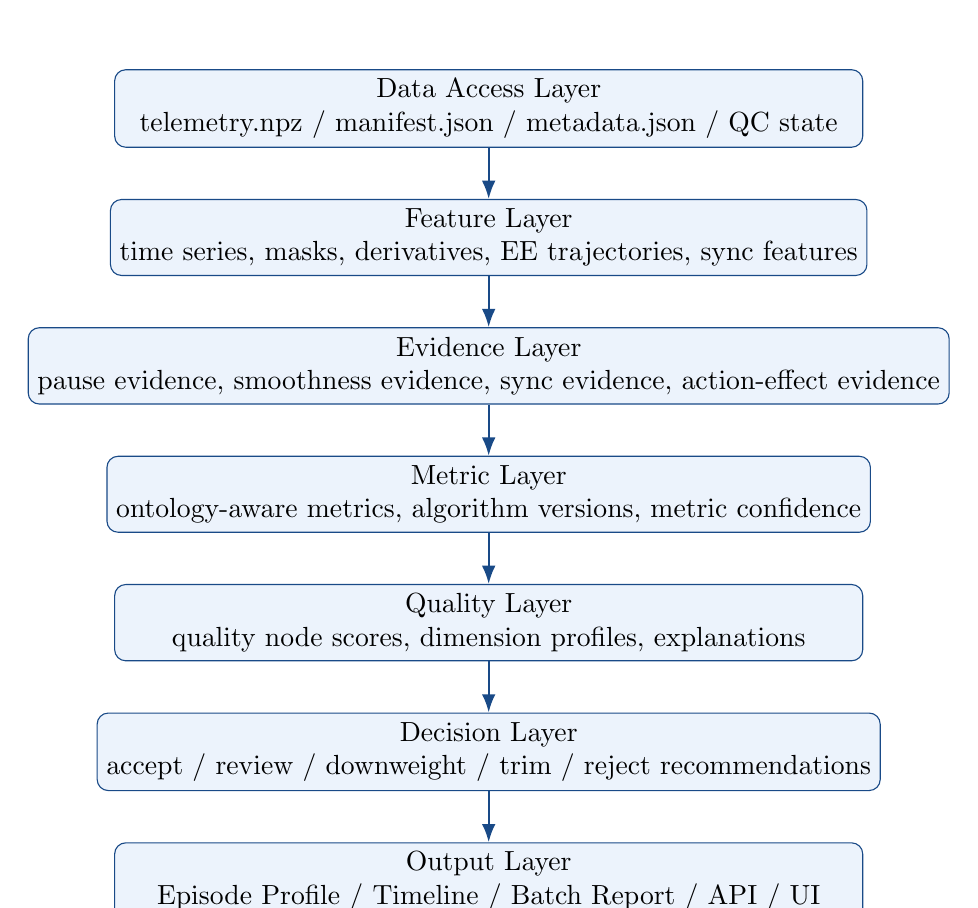
\begin{tikzpicture}[
  node distance=0.65cm,
  box/.style={rectangle,draw=RuleBlue,rounded corners,align=center,minimum width=9.5cm,minimum height=0.72cm,fill=LightBlue},
  arr/.style={-Latex,thick,draw=RuleBlue}
]
\node[box] (data) {Data Access Layer\\telemetry.npz / manifest.json / metadata.json / QC state};
\node[box,below=of data] (feature) {Feature Layer\\time series, masks, derivatives, EE trajectories, sync features};
\node[box,below=of feature] (evidence) {Evidence Layer\\pause evidence, smoothness evidence, sync evidence, action-effect evidence};
\node[box,below=of evidence] (metric) {Metric Layer\\ontology-aware metrics, algorithm versions, metric confidence};
\node[box,below=of metric] (quality) {Quality Layer\\quality node scores, dimension profiles, explanations};
\node[box,below=of quality] (decision) {Decision Layer\\accept / review / downweight / trim / reject recommendations};
\node[box,below=of decision] (report) {Output Layer\\Episode Profile / Timeline / Batch Report / API / UI};
\draw[arr] (data) -- (feature);
\draw[arr] (feature) -- (evidence);
\draw[arr] (evidence) -- (metric);
\draw[arr] (metric) -- (quality);
\draw[arr] (quality) -- (decision);
\draw[arr] (decision) -- (report);
\end{tikzpicture}
\end{center}

\subsection{核心思想}

Engine v2 的核心思想可以概括为三句话：

\begin{enumerate}
\item \Term{Feature 是计算复用层}：所有算法共享同一套基础特征，避免重复读取 MinIO 和重复计算导数、mask、分段。
\item \Term{Evidence 是解释层}：每一个质量判断都必须能回溯到一组证据，而不是只给出一个不可解释分数。
\item \Term{Quality 是业务语义层}：前端、报告、数据库和数据集发布不直接面向算法名称，而面向质量本体节点。
\end{enumerate}

\section{数据输入层}

\subsection{输入文件}

L3 v2 主要依赖 TeleDex processed 数据。输入优先级如下：

\begin{longtable}{L{4cm} L{4cm} L{6cm}}
\toprule
输入 & 用途 & 说明 \\
\midrule
\Code{telemetry.npz} & 核心时序数据 & 包含 qpos、qvel、actions、effort、timestamps、sync、EE pose、IMU 等。 \\
\Code{manifest.json} & 快速元数据 & 提供 fps、duration、frame count、collect depth/tactile/imu 等字段。 \\
\Code{metadata.json} & 对齐和转换信息 & 提供 alignment、sensor offsets、valid time range、conversion 配置。 \\
\Code{camera\_info.json} & 相机标定信息 & 当前阶段主要用于扩展，不作为 L3 motion 计算核心输入。 \\
数据库 Episode 元数据 & 任务上下文 & 包含批次、任务、episode 编号、人工 QC 状态、原因码等。 \\
L2/L4 结果 & 跨层证据 & 可作为 Observation Quality 与 Task Quality 的外部证据。 \\
\bottomrule
\end{longtable}

\subsection{Data Access Layer 职责}

Data Access Layer 应统一负责 MinIO 读取、文件存在性检查、npz 解析、JSON 解析、数据裁剪、dtype 校验和基础异常处理。上层模块不应直接访问 MinIO。

\begin{verbatim}
class EpisodeDataBundle:
    episode_id: int
    telemetry: TelemetryData
    manifest: ManifestData | None
    metadata: MetadataData | None
    episode_meta: EpisodeMeta
    l2_result: Optional[L2Result]
    l4_result: Optional[L4Result]
\end{verbatim}

\subsection{输入校验}

输入校验不直接给训练质量打分，而是决定该 episode 是否可以进入计算流程。建议分为：

\begin{itemize}
\item \Term{fatal}：缺失 telemetry、timestamps 非单调、qpos/actions 维度无法对齐。
\item \Term{degraded}：缺失 effort、缺失 EE pose、缺失 IMU、manifest 与 telemetry 帧数不一致但可恢复。
\item \Term{warning}：fps 异常、duration 过短、sync metadata 缺失、部分维度全零。
\end{itemize}

\section{Feature Layer 设计}

\subsection{Feature Layer 的必要性}

在 L3 v1 中，多个指标会重复计算类似的中间量，例如 arm/hand 维度划分、零值维度 mask、dt、速度、加速度、jerk、低动作 mask、饱和 mask 等。v2 应将这些内容统一抽象为 Feature Layer。

\subsection{FeatureBundle}

建议定义 \Code{FeatureBundle} 作为核心中间对象：

\begin{verbatim}
class FeatureBundle:
    time: TimeFeatures
    joint: JointFeatures
    action: ActionFeatures
    ee: EndEffectorFeatures | None
    hand: HandFeatures | None
    sync: SyncFeatures | None
    imu: ImuFeatures | None
    masks: ValidityMasks
    metadata: FeatureMetadata
\end{verbatim}

\subsection{基础特征清单}

\begin{longtable}{L{3.5cm} L{4.5cm} L{6cm}}
\toprule
特征组 & 输出 & 用途 \\
\midrule
TimeFeatures & t, dt, fps, duration, frame count, jitter & 时间连续性、窗口计算、timeline 对齐。 \\
JointFeatures & arm/hand split, qpos valid dims, qvel, derivatives & 平滑度、连续性、运动强度、运动范围。 \\
ActionFeatures & action delta, action velocity, action magnitude, action masks & 动作信息量、动作有效性、操作犹豫、饱和诊断。 \\
EndEffectorFeatures & position, orientation, velocity, path length, jerk & 任务空间平滑度、轨迹效率、末端稳定性。 \\
HandFeatures & finger positions, deltas, reversals, coordination features & 灵巧操作质量、手指颤振、抓取动作信息量。 \\
SyncFeatures & sync valid mask, max diff, invalid spans & 数据完整性与观测可对齐性。 \\
ImuFeatures & acceleration norm, angular velocity norm, spikes & 抖动、碰撞、相机/末端不稳定诊断。 \\
ValidityMasks & valid frames, zero dims, clipped dims, missing spans & 所有上层计算的可靠性控制。 \\
\bottomrule
\end{longtable}

\subsection{Feature 缓存策略}

Feature 可作为轻量缓存，但不一定需要全部持久化。推荐策略：

\begin{itemize}
\item 对 episode 打开频繁、文件大、计算慢的特征持久化。
\item 对低成本导数和 mask 可运行时计算。
\item 对 EE trajectory、window aggregation、timeline candidate spans 优先缓存。
\item 所有缓存都必须绑定 \Code{feature\_version} 和源文件 checksum。
\end{itemize}

\section{Evidence Layer 设计}

\subsection{EvidenceRecord}

Evidence 是 L3 v2 的解释核心。每条 EvidenceRecord 表达一个可解释事实，而不是最终分数。

\begin{verbatim}
class EvidenceRecord:
    evidence_id: str
    ontology_node: str
    evidence_type: str
    severity: str
    confidence: float
    value: float | dict
    time_spans: list[TimeSpan]
    source_features: list[str]
    algorithm_version: str
    message: str
\end{verbatim}

\subsection{Evidence 类型}

\begin{longtable}{L{3.5cm} L{4cm} L{6.5cm}}
\toprule
Evidence 类型 & 示例 & 说明 \\
\midrule
Positive Evidence & 有效操作密度高、关键动作清晰 & 支持数据进入训练集的证据。 \\
Negative Evidence & 长时间停顿、手指颤振、同步异常 & 支持复核、降权或剔除的证据。 \\
Diagnostic Evidence & Tracking error 高、effort spike & 不直接决定训练价值，但帮助解释机械或控制异常。 \\
Coverage Evidence & 轨迹覆盖新区域、动作多样性高 & 主要用于 dataset 级分析。 \\
Integrity Evidence & 缺帧、时间戳抖动、传感器不同步 & 支持数据是否可训练的硬性判断。 \\
\bottomrule
\end{longtable}

\subsection{Evidence 与 Timeline}

Timeline 不应只展示异常。v2 timeline 应包含至少四类片段：

\begin{itemize}
\item \Term{negative spans}：异常、低质量、不可训练片段。
\item \Term{low-information spans}：长时间无有效学习信号，可用于裁剪或降权。
\item \Term{key-action spans}：抓取、接触、放置、快速状态变化等高价值片段。
\item \Term{review spans}：系统不确定、需要人工重点看的片段。
\end{itemize}

\section{Metric Layer 设计}

\subsection{MetricResult}

Metric 是 Evidence 的数值化聚合。每一个 Metric 必须绑定 Ontology Node 和 Algorithm Version。

\begin{verbatim}
class MetricResult:
    metric_id: str
    metric_name: str
    ontology_node: str
    algorithm_id: str
    algorithm_version: str
    value: float | dict
    score: float | None
    severity: str | None
    confidence: float
    evidence_refs: list[str]
    time_spans: list[TimeSpan]
    explanation: str
\end{verbatim}

\subsection{Metric Registry}

Metric Registry 是系统可扩展性的关键。推荐维护如下字段：

\begin{longtable}{L{4cm} L{9.5cm}}
\toprule
字段 & 含义 \\
\midrule
metric\_id & 稳定 ID，例如 MQ-SMOOTH-001。 \\
metric\_name & 面向 UI 和报告的名称。 \\
ontology\_node & 挂载到哪一个质量本体节点。 \\
input\_features & 依赖哪些 Feature。 \\
output\_schema & 输出 value/score/confidence/time spans 的结构。 \\
default\_algorithm & 当前默认算法。 \\
candidate\_algorithms & 可替代算法列表。 \\
training\_impact & 为什么影响模型学习。 \\
timeline\_support & 是否支持时间窗定位。 \\
version & Metric 定义版本。 \\
\bottomrule
\end{longtable}

\subsection{v1 指标迁移}

\begin{longtable}{L{3.4cm} L{4.4cm} L{5.8cm}}
\toprule
v1 指标 & v2 去向 & 说明 \\
\midrule
LDLJ & Motion Smoothness evidence/metric & 保留但不再作为唯一平滑度指标；后续加入 EE smoothness 和 SPARC。 \\
Dead Actions & Information Density / Low-action Evidence & 从“无效动作错误”改为“低学习信号片段”。 \\
Static & Pause / Low-information Evidence & 与 Dead 合并到低信息和停顿体系，减少重复扣分。 \\
Saturation & Action Validity Diagnostic & 手部 0/255 可能合法，需按任务和动态变化判断。 \\
Jitter & Data Integrity Metric & 仍作为硬性数据完整性指标。 \\
Tracking Error & Execution Diagnostic & 降级为诊断证据，不再作为训练质量主指标。 \\
Chatter & Dexterity / Hand Stability Metric & 保留并改进 timeline 合并和频域检测。 \\
Effort & Physical Stress Diagnostic & 用于异常负载诊断，不作为训练质量核心分。 \\
Q\_motion & Dimension scores + Training Suitability & 不再用一个运动分代表全部质量。 \\
\bottomrule
\end{longtable}

\section{Quality Layer 设计}

\subsection{QualityNodeScore}

Quality Layer 将多个 Metrics 聚合到质量本体节点上。

\begin{verbatim}
class QualityNodeScore:
    node_id: str
    node_name: str
    parent_node_id: str | None
    score: float | None
    severity: str
    confidence: float
    metric_refs: list[str]
    evidence_refs: list[str]
    explanation: str
    recommendation: str | None
\end{verbatim}

\subsection{质量维度示例}

\begin{longtable}{L{4cm} L{4cm} L{5.7cm}}
\toprule
一级维度 & 二级节点 & 主要 Evidence \\
\midrule
Learnability & Information Density & 有效动作比例、低信息片段、关键动作密度。 \\
Demonstration Quality & Smoothness / Continuity / Efficiency & joint/EE jerk、暂停、路径绕行、速度连续性。 \\
Motion Quality & Stability / Dexterity & 抖动、反向翻转、手指协调、末端稳定。 \\
Observation Quality & Temporal Alignment & sync validation、timestamp jitter、跨模态对齐。 \\
Data Integrity & Completeness / Consistency & 文件完整性、帧数一致性、维度有效性。 \\
Task Quality & Completeness / Semantic Alignment & L4 结果、人工复核、未来 VLM 证据。 \\
\bottomrule
\end{longtable}

\section{Fusion 与 Decision Layer}

\subsection{为什么不直接做一个总分}

一个总分容易隐藏关键信息。对于训练数据，错误类型不同，处理方式也不同。例如同步错误可能需要剔除；长时间低信息片段可能可以裁剪；轻微动作不平滑可以降权；任务未完成需要 L4 判断。因此 v2 应优先输出质量画像，再输出准入建议。

\subsection{推荐输出}

\begin{itemize}
\item \Code{training\_suitability\_score}：面向训练集筛选的综合建议分。
\item \Code{dimension\_scores}：按 Ontology 维度输出的质量画像。
\item \Code{hard\_gates}：数据完整性、同步错误、极端缺失等硬性门控。
\item \Code{recommendation}：accept / review / trim / downweight / reject。
\item \Code{confidence}：系统对该建议的可靠性。
\end{itemize}

\subsection{决策规则}

第一阶段建议采用规则融合，不直接训练质量判别模型。规则融合应遵循：

\begin{enumerate}
\item 硬性数据完整性问题优先于所有软性评分。
\item L4 任务失败优先于运动质量评分。
\item 可裁剪的低信息片段不直接导致整条拒绝。
\item 诊断类指标只影响 review 优先级，不直接决定训练准入。
\item score 必须伴随 explanation 和 evidence refs。
\end{enumerate}

\section{Timeline Layer 设计}

\subsection{TimelineSegment v2}

\begin{verbatim}
class TimelineSegment:
    segment_id: str
    start_time: float
    end_time: float
    segment_type: str
    severity: str
    ontology_node: str
    evidence_refs: list[str]
    metric_refs: list[str]
    label: str
    description: str
    suggested_action: str | None
\end{verbatim}

\subsection{Segment 类型}

\begin{longtable}{L{3.5cm} L{4cm} L{6cm}}
\toprule
类型 & UI 标签 & 用途 \\
\midrule
anomaly & 异常段 & 同步异常、剧烈抖动、不可解释突变。 \\
low\_information & 低信息段 & 长时间无有效动作，可建议裁剪或降权。 \\
key\_action & 关键动作段 & 抓取、放置、接触、状态突变等高学习价值段。 \\
review & 复核段 & 系统不确定或多证据冲突，需要人工查看。 \\
diagnostic & 诊断段 & 高 tracking error、高 effort 等非训练质量主问题。 \\
\bottomrule
\end{longtable}

\section{Report Layer 设计}

\subsection{EpisodeQualityProfile}

Episode 层输出应替代当前简单的 metrics 数组。

\begin{verbatim}
class EpisodeQualityProfile:
    episode_id: int
    engine_version: str
    ontology_version: str
    run_id: str
    summary: QualitySummary
    quality_nodes: list[QualityNodeScore]
    metrics: list[MetricResult]
    evidence: list[EvidenceRecord]
    timeline: list[TimelineSegment]
    diagnostics: list[DiagnosticItem]
    recommendation: Recommendation
\end{verbatim}

\subsection{BatchQualityProfile}

Batch 层输出用于数据集发布和阈值标定。

\begin{itemize}
\item 指标分布：每个 metric 的 P50/P75/P90/P95/P99。
\item 质量分布：各质量维度的通过率、复核率、拒绝率。
\item 异常模式：高频异常类型、任务类型差异、批次采集偏移。
\item 代表样本：top good、top bad、边界样本、人工复核样本。
\item 发布建议：可训练、需抽检、需重采、需任务类型标定。
\end{itemize}

\section{缓存与数据库设计}

\subsection{缓存目标}

缓存不是为了单纯加速页面，而是为了让质量结果成为可追溯的数据资产。每一次 engine run 都应有版本号、参数快照和输入文件标识。

\subsection{建议表结构}

\begin{longtable}{L{4cm} L{9.5cm}}
\toprule
表名 & 作用 \\
\midrule
\Code{quality\_engine\_runs} & 每次 L3 v2 计算运行记录，保存 engine version、ontology version、metric library version、config hash。 \\
\Code{quality\_features\_cache} & 可选特征缓存，保存 feature bundle 元信息和对象存储路径。 \\
\Code{quality\_evidence} & EvidenceRecord 持久化表。 \\
\Code{quality\_metric\_results} & MetricResult 持久化表。 \\
\Code{quality\_node\_scores} & Ontology 节点评分表。 \\
\Code{quality\_timeline\_segments} & TimelineSegment 表。 \\
\Code{quality\_recommendations} & 准入建议、处理动作和人工确认状态。 \\
\Code{quality\_algorithm\_registry} & 算法版本、默认启用状态和参数 schema。 \\
\bottomrule
\end{longtable}

\subsection{缓存失效规则}

以下事件必须触发重新计算：

\begin{itemize}
\item telemetry 或 metadata 文件 checksum 变化。
\item ontology version 变化。
\item metric definition 变化。
\item algorithm version 变化。
\item scoring / threshold config 变化。
\item 任务类型标定参数变化。
\end{itemize}

\section{API 设计}

\subsection{Episode API}

\begin{longtable}{L{5cm} L{8.5cm}}
\toprule
API & 说明 \\
\midrule
\Code{GET /api/episodes/{id}/quality-profile} & 返回 EpisodeQualityProfile，是前端主入口。 \\
\Code{GET /api/episodes/{id}/quality-timeline} & 返回 timeline segments，可用于播放器和曲线联动。 \\
\Code{POST /api/episodes/{id}/quality/recompute} & 强制重算，管理员或后台任务使用。 \\
\Code{GET /api/episodes/{id}/quality-evidence} & 返回可展开证据树，供调试和高级 UI 使用。 \\
\Code{GET /api/episodes/{id}/telemetry-features} & 返回降采样特征曲线，不直接暴露全部 telemetry。 \\
\bottomrule
\end{longtable}

\subsection{Batch API}

\begin{longtable}{L{5cm} L{8.5cm}}
\toprule
API & 说明 \\
\midrule
\Code{POST /api/batches/{id}/quality/run} & 启动批次质量计算。 \\
\Code{GET /api/batches/{id}/quality-report} & 获取批次质量报告。 \\
\Code{GET /api/batches/{id}/quality-distribution} & 获取质量分布和同类对比。 \\
\Code{GET /api/batches/{id}/representative-episodes} & 获取代表性样本列表。 \\
\bottomrule
\end{longtable}

\section{前端集成设计}

\subsection{Manual QC 页面变化}

L3 v2 后，人工 QC 页面不应只展示一个 Q\_motion 环和若干指标卡片。建议改为：

\begin{itemize}
\item 顶部显示 Training Suitability 与硬性门控状态。
\item 右侧显示质量维度树，而不是平铺指标卡片。
\item 每个质量维度可展开，显示证据、指标和解释。
\item 播放进度条上叠加多类型 timeline segments。
\item 曲线图支持点击 evidence 自动定位并高亮相关特征。
\item 提交区允许审核员确认或纠正系统建议，用于后续标定。
\end{itemize}

\subsection{质量画像 UI}

推荐 UI 结构：

\begin{verbatim}
Training Suitability
  - Accept / Review / Trim / Downweight / Reject

Quality Tree
  Learnability
    Information Density
    Action Effectiveness
  Demonstration Quality
    Smoothness
    Continuity
    Efficiency
  Data Integrity
    Sync
    Temporal Consistency

Evidence Timeline
  Key Action / Low Information / Anomaly / Review / Diagnostic
\end{verbatim}

\section{后台任务与运行模式}

\subsection{运行模式}

L3 v2 支持三种运行模式：

\begin{longtable}{L{3cm} L{4cm} L{6.5cm}}
\toprule
模式 & 场景 & 说明 \\
\midrule
On-demand & 打开单条 episode & 缓存命中时直接返回；缺失时快速计算核心 profile。 \\
Offline batch & 批次导入后 & 后台计算完整 profile、timeline、batch distribution。 \\
Calibration run & 阈值标定 & 使用 approved samples 重跑指标分布，不一定写入生产结果。 \\
\bottomrule
\end{longtable}

\subsection{任务队列}

建议引入后台任务队列，例如 Celery/RQ/Arq，或先用 FastAPI BackgroundTasks 作为过渡。批次计算不应阻塞人工 QC 页面。

\section{Python 包结构建议}

建议后端新增独立模块：

\begin{verbatim}
backend/app/services/rddqf/
    __init__.py
    engine.py
    data_access.py
    feature_extraction/
        time_features.py
        joint_features.py
        action_features.py
        ee_features.py
        hand_features.py
        sync_features.py
    evidence/
        evidence_types.py
        smoothness_evidence.py
        low_info_evidence.py
        sync_evidence.py
        dexterity_evidence.py
    metrics/
        registry.py
        motion_metrics.py
        learnability_metrics.py
        integrity_metrics.py
    quality/
        ontology_registry.py
        quality_fusion.py
        recommendations.py
    timeline/
        segment_builder.py
        span_merge.py
    persistence/
        result_store.py
        cache.py
    schemas.py
    config.py
\end{verbatim}

\section{与现有系统的兼容}

\subsection{API 兼容策略}

第一阶段可以保留旧的 \Code{/qc-context} 返回结构，同时新增 \Code{qualityProfile} 字段。前端可以逐步迁移，避免一次性重构全部页面。

\subsection{v1 指标保留策略}

v1 的 8 个指标不应一次性删除。推荐：

\begin{enumerate}
\item 第一阶段作为 v2 evidence/diagnostic 的一部分保留。
\item 第二阶段调整命名、分组和权重。
\item 第三阶段引入更合理的算法替代，例如 EE smoothness、SPARC、信息密度等。
\item 第四阶段通过标定数据决定是否彻底下线旧指标。
\end{enumerate}

\section{实现路线图}

\subsection{Milestone 1：最小可用 L3 v2}

\begin{itemize}
\item 建立 EpisodeDataBundle 和 FeatureBundle。
\item 实现 Time、Joint、Action、Sync 基础特征。
\item 将 v1 指标迁移为 MetricResult。
\item 新增 EvidenceRecord 和 TimelineSegment v2。
\item API 返回 qualityProfile，但前端可继续兼容旧卡片。
\end{itemize}

\subsection{Milestone 2：Evidence-driven UI}

\begin{itemize}
\item 前端右侧改为质量维度树。
\item timeline 支持多类型 segment。
\item 曲线图支持 evidence 高亮。
\item 审核员可确认系统建议和纠正原因。
\end{itemize}

\subsection{Milestone 3：离线缓存与批次报告}

\begin{itemize}
\item 增加 quality result tables。
\item 批次导入后后台计算 quality profile。
\item 生成 batch distribution 和代表样本列表。
\item 初步支持同类任务对比。
\end{itemize}

\subsection{Milestone 4：数据驱动标定}

\begin{itemize}
\item 使用 approved samples 做分布统计。
\item 按任务类型建立阈值组。
\item 将 Good/Warn/Bad 从经验值迁移到 percentile-based calibration。
\item 将人工复核反馈进入阈值迭代流程。
\end{itemize}

\section{风险与缓解}

\begin{longtable}{L{4cm} L{4cm} L{5.8cm}}
\toprule
风险 & 表现 & 缓解 \\
\midrule
架构过度复杂 & 实现周期拉长 & 先做最小 v2，所有层可以轻量对象实现。 \\
指标过多 & UI 信息过载 & 面向 Ontology 展示，只默认显示维度分和关键证据。 \\
阈值不稳定 & Good/Warn/Bad 误判 & 初期弱化自动 reject，强调 review 和证据展示。 \\
计算性能压力 & 大 episode 打开慢 & Feature 缓存、离线批处理、按需返回 summary。 \\
旧系统迁移风险 & 前端/后端同时改动大 & 保持旧 API 兼容，逐步引入 qualityProfile。 \\
\bottomrule
\end{longtable}

\section{结论}

L3MetricsEngine v2 的核心价值不是新增若干指标，而是建立一套可解释、可版本化、可缓存、可扩展的数据质量计算架构。它将当前 L3 从“episode 打开时计算运动指标”升级为“机器人训练数据质量评价引擎”。

从下一阶段开始，项目应转入工程实现：先构建 Feature Layer 和 Evidence Layer 的最小版本，再将 v1 指标迁移到新架构中，最后逐步替换算法、重构 UI、引入缓存和批次报告。此路径可以在不打断现有人工 QC 工作流的前提下，让系统逐渐具备面向机器人数据资产平台的能力。


\newpage
\section*{v1.1 实现要求：引擎新增能力}
\addcontentsline{toc}{section}{v1.1 实现要求：引擎新增能力}

实现阶段需在 L3MetricsEngine v2 中增加以下能力：

\begin{enumerate}
\item Feature Layer 增加 \Code{joint\_jerk\_norm}, \Code{action\_delta2\_norm}, \Code{effective\_action\_mask}, \Code{robust\_timestamp\_features}, \Code{adaptive\_sync\_features}, \Code{camera\_frame\_features}。
\item Evidence Layer 支持 sensor-specific evidence，尤其是 wrist camera severe desync 与 camera freeze。
\item Metric Layer 按 v1.1 更新 MQ/LQ/DI/DX 计算逻辑，并新增 DI-03/OQ-01。
\item Timeline Engine 支持 metric timeline 与 diagnostic timeline 分离，并支持 affected sensor、capture time、sync offset、possible cause。
\item Quality Layer 将 DX-01 排除在 Training Quality Score 之外；Data Integrity 同时作为加权项与 reliability gate。
\item API 增加 \Code{reliabilityWarnings}, \Code{diagnosticWarnings}, \Code{executionDiagnosticScore}, \Code{cameraFrameDiagnostics}。
\end{enumerate}

\subsection*{推荐输出结构}

\begin{quote}\small
\Code{trainingQualityScore}, \Code{motionQualityScore}, \Code{learnabilityScore}, \Code{dataIntegrityScore}, \Code{executionDiagnosticScore}, \Code{qualityDimensions}, \Code{metricResults}, \Code{diagnosticMetrics}, \Code{reliabilityWarnings}, \Code{diagnosticWarnings}, \Code{timelineSegments}, \Code{cameraFrameDiagnostics}
\end{quote}

\subsection*{前端解释性要求}

严重同步错位不应只显示为 Bad，而应解释为：哪一路 sensor、真实采集时刻、落后主时间轴多少毫秒、持续多久、是否可能是 stale frame 或 frame freeze。Execution Diagnostics 必须标注：仅作为执行链路诊断，不参与训练质量总分。

\clearpage

\chapter{总体架构 v2}

\section{项目定位的根本转变}

\subsection{从 Motion QC 到 Training Data QC}

原有 L3 v1 的潜在目标是评价遥操作轨迹的运动执行质量，因此自然产生了 LDLJ、Tracking Error、Dead Action、Static、Saturation、Jitter、Chatter、Effort 等指标。这些指标在机器人控制和采集诊断中有价值，但它们不完全等价于“这条数据是否适合训练模型”。

面向 VLA、模仿学习和机器人基础模型时，训练数据更重要的问题是：

\begin{itemize}
\item demonstration 是否成功表达了任务意图？
\item observation-action 序列是否连续、可学习、信息量充足？
\item 动作是否自然、稳定、没有无意义抖动和大量犹豫？
\item 数据是否同步、完整、可对齐？
\item 这条 episode 在整个数据集中是否有贡献，而不是冗余？
\end{itemize}

因此，RDDQF 的评价对象不是机器人本体，也不是控制器，而是 demonstration 作为训练数据资产的价值。

\begin{notebox}{核心命题}
L3 的目标不是评价机器人执行得有多好，而是评价记录下来的 demonstration 对下游策略学习有多大价值。
\end{notebox}

\subsection{为什么 Tracking Error 不能作为核心质量指标}

在 TeleDex 数据中，\Code{actions} 表示遥操作设备发送的目标关节位置，\Code{qpos} 表示机器人实际反馈位置。\Code{|actions-qpos|} 衡量的是命令跟踪误差，主要反映控制执行或机械响应，而不是 demonstration 本身的训练价值。

如果一条数据视频清晰、动作自然、任务完成、学习信号充分，但机器人控制器略有滞后，它仍可能是优质训练数据。反之，如果控制器跟踪完美，但操作者反复犹豫、动作抖动、任务失败，它并不是优质 demonstration。因此，Tracking Error 在新框架中应被降级为 Diagnostic Evidence，而不是训练质量主指标。

\section{RDDQF 文档体系}

\subsection{文档栈}

\begin{center}
\begin{tikzpicture}[
  node distance=0.62cm,
  box/.style={rectangle,draw=RuleBlue,rounded corners,align=center,minimum width=10.2cm,minimum height=0.72cm,fill=LightBlue},
  arr/.style={-Latex,thick,draw=RuleBlue}
]
\node[box] (std) {01 Training Data Quality Standard\\定义什么叫高质量训练数据};
\node[box,below=of std] (onto) {02 Quality Ontology\\定义高质量由哪些质量维度组成};
\node[box,below=of onto] (ev) {03 Evidence Specification\\定义每个质量判断需要哪些证据};
\node[box,below=of ev] (met) {04 Metric Library\\定义可选指标库和指标语义};
\node[box,below=of met] (eng) {05 L3MetricsEngine v2 Architecture\\定义如何把框架落地到后端、API、UI 和缓存};
\draw[arr] (std) -- (onto);
\draw[arr] (onto) -- (ev);
\draw[arr] (ev) -- (met);
\draw[arr] (met) -- (eng);
\end{tikzpicture}
\end{center}

\subsection{当前文档清单}

\begin{longtable}{L{4.3cm} L{3cm} L{6.5cm}}
\toprule
文档 & 状态 & 作用 \\
\midrule
Training Data Quality Standard v1.0 & 已完成 & 定义训练数据质量的目标、哲学、边界和基本原则。 \\
Robot Demonstration Quality Ontology v1.0 & 已完成 & 建立 Learnability、Demonstration Quality、Motion Quality、Observation Quality、Data Integrity、Diversity 等质量本体。 \\
Robot Demonstration Quality Evidence Specification v1.0 & 已完成 & 定义 Positive/Negative/Diagnostic/Coverage/Integrity Evidence，并将质量判断转化为可解释证据。 \\
Robot Demonstration Metric Library v1.0 & 已完成 & 按质量本体组织候选指标，不把 LDLJ/Tracking 等旧指标作为第一对象。 \\
L3MetricsEngine v2 System Architecture v1.0 & 本轮完成 & 定义工程分层、数据契约、缓存、API、UI 接入和实现路线。 \\
RDDQF Overall Architecture v2.0 & 本文档 & 统一整套思想，明确理论阶段结束和工程阶段路线。 \\
\bottomrule
\end{longtable}

\section{五层思想链路}

\subsection{Standard：定义质量目标}

Standard 解决的是最根本的问题：什么样的机器人 demonstration 值得进入训练集。它不讨论公式、不讨论代码、不讨论阈值，只定义评价哲学。

核心原则包括：

\begin{itemize}
\item 质量由可学习性定义，而不是由执行精度定义。
\item 评价对象是 demonstration，不是机器人硬件。
\item 评价的是 learning signal，而不是机械物理量本身。
\item 所有指标都必须能说明它为什么影响下游模型学习。
\end{itemize}

\subsection{Ontology：定义质量维度}

Ontology 将抽象质量目标拆解为稳定的质量树。它是后续所有指标、UI、报告和数据库的共同语义基础。

一套简化的一级结构如下：

\begin{verbatim}
Robot Demonstration Quality
  Learnability
  Demonstration Quality
  Motion Quality
  Observation Quality
  Data Integrity
  Task Quality
  Diversity and Coverage
\end{verbatim}

Ontology 的价值在于稳定性。算法会变，阈值会变，指标会变，但质量节点应保持相对稳定。

\subsection{Evidence：定义解释依据}

Evidence 是 RDDQF 区别于传统指标系统的关键。传统系统给出“LDLJ=7.2”，但不能充分解释为什么这条数据适合或不适合训练。Evidence Layer 要求每个质量判断都能回溯到具体证据，例如：

\begin{itemize}
\item 有效动作密度低，说明学习信号不足。
\item 末端轨迹平滑，说明动作示范自然。
\item 同步误差持续超过阈值，说明 observation-action 对齐不可靠。
\item 手指快速反复翻转，说明灵巧手动作存在抖动。
\item 关键动作段清晰，说明该片段具有较高训练价值。
\end{itemize}

\subsection{Metric：定义可计算表达}

Metric Library 将证据进一步数值化。它不是最终算法规范，而是候选指标集合。一个质量节点可以由多个指标支持，一个指标也可以有多个算法实现。

例如 Smoothness 可以由 joint jerk、EE jerk、SPARC、频域能量等指标表达。不同阶段可以先实现简单指标，再替换为更鲁棒算法。

\subsection{Engine：定义工程实现}

Engine Architecture 将前面的理论对象落地为后端架构。其核心分层是：

\begin{verbatim}
Data Access
  -> Feature Extraction
  -> Evidence Extraction
  -> Metric Computation
  -> Quality Scoring
  -> Decision Recommendation
  -> Timeline / Report / Cache
\end{verbatim}

这使 RDDQF 从文档框架变成可以实现的系统架构。

\section{与现有 L1-L4 质检体系的关系}

\subsection{L1：硬性门控}

L1 仍由上游采集或平台硬性门控负责。L3 v2 可以读取 L1 结果作为 Data Integrity 的先验，不重复做采集侧不可恢复问题的判定。

\subsection{L2：视觉质量}

L2 负责视觉模糊、过曝、遮挡、深度异常等人工判断。RDDQF 中的 Observation Quality 可以吸收 L2 结果作为 Evidence。未来也可以将 L2 自动化指标纳入同一质量本体。

\subsection{L3：训练数据质量}

L3 v2 是 RDDQF 在当前系统中的核心落地点。它以 telemetry、metadata、manifest、L2/L4 结果为输入，输出 episode quality profile、timeline evidence、训练准入建议和批次报告。

\subsection{L4：任务完成度}

L4 是 Task Quality 的关键来源。当前 L4 由人工判断，未来可通过 VLM 或任务状态检测辅助。L3 v2 不替代 L4，而是将 L4 结果作为最高权重的任务证据之一。

\section{系统总体架构}

\subsection{数据链路}

\begin{verbatim}
TeleDex raw mcap
    -> TeleDex processed conversion
    -> MinIO processed episode files
    -> PostgreSQL episode metadata
    -> RDDQF / L3MetricsEngine v2
    -> Quality Result Store
    -> Manual QC UI
    -> Batch Quality Report
    -> Dataset Release Pipeline
    -> Foundation Model Training
\end{verbatim}

\subsection{业务闭环}

RDDQF 不是一次性评分系统，而是闭环系统：

\begin{enumerate}
\item 采集系统产生数据。
\item L3 v2 自动生成质量画像。
\item 人工 QC 审核系统建议。
\item 审核结果反哺阈值标定和算法验证。
\item 批次报告决定数据集发布策略。
\item 训练表现反过来验证质量指标有效性。
\end{enumerate}

\section{质量结果的数据资产化}

\subsection{为什么质量结果必须持久化}

如果质量结果只在打开页面时临时计算，它就只是 UI 辅助信息。若要成为数据资产平台的一部分，质量结果必须持久化、版本化、可追溯。

\subsection{质量资产包括什么}

\begin{itemize}
\item Episode 级 Quality Profile。
\item Evidence Records 和 Timeline Segments。
\item Metric Results 与 Algorithm Version。
\item Batch Quality Distribution。
\item Dataset Release Report。
\item 人工审核反馈和标定样本集合。
\end{itemize}

\subsection{版本化要求}

任何质量结果都必须绑定：

\begin{itemize}
\item ontology version；
\item metric library version；
\item algorithm version；
\item threshold config version；
\item source data checksum；
\item engine run id。
\end{itemize}

\section{工程阶段总体路线}

\subsection{Phase I：理论阶段（已完成）}

本阶段完成文档：

\begin{itemize}
\item Training Data Quality Standard。
\item Quality Ontology。
\item Evidence Specification。
\item Metric Library。
\item L3MetricsEngine v2 Architecture。
\item Overall Architecture v2。
\end{itemize}

\subsection{Phase II：Engine 最小实现}

目标是让 v2 架构跑起来，而不是一次性实现所有指标。建议最小实现包括：

\begin{itemize}
\item Data Access Layer。
\item FeatureBundle。
\item EvidenceRecord。
\item MetricResult。
\item QualityNodeScore。
\item TimelineSegment v2。
\item 将 v1 指标迁移到 v2 输出结构。
\end{itemize}

\subsection{Phase III：UI 与 API 迁移}

目标是在不破坏现有人工 QC 流程的情况下，逐步将前端从指标卡片迁移到质量画像。

\begin{itemize}
\item 新增 \Code{qualityProfile} API。
\item 前端保留旧卡片，增加质量树视图。
\item Timeline 支持多类型 segment。
\item 曲线图与 evidence 联动。
\end{itemize}

\subsection{Phase IV：离线缓存与批次报告}

目标是让质量评价服务批次和数据集，而不是只服务单条 episode。

\begin{itemize}
\item 建立 quality result tables。
\item 批次后台计算。
\item 指标分布统计。
\item 代表样本抽取。
\item 同类任务基线对比。
\end{itemize}

\subsection{Phase V：标定与数据发布}

目标是从经验阈值升级为数据驱动阈值，并支持训练数据集发布。

\begin{itemize}
\item approved sample 标定。
\item 按任务类型建立阈值组。
\item 数据集发布质量报告。
\item 训练表现回流验证。
\end{itemize}

\section{下一步具体落地操作}

\subsection{立即执行的工程任务}

理论阶段完成后，下一步不再新增框架文档，而是开始代码层落地。建议第一批任务如下：

\begin{enumerate}
\item 在后端新增 \Code{backend/app/services/rddqf/} 包。
\item 定义核心 schema：\Code{FeatureBundle}、\Code{EvidenceRecord}、\Code{MetricResult}、\Code{QualityNodeScore}、\Code{EpisodeQualityProfile}。
\item 实现 Data Access Layer，统一读取 telemetry、manifest、metadata。
\item 实现 Time/Joint/Action/Sync 四类基础 Feature。
\item 将当前 8 个 v1 指标迁移为 v2 MetricResult 和 EvidenceRecord。
\item 新增 \Code{/quality-profile} API，暂时与旧 \Code{/qc-context} 并行。
\item 前端先展示 v2 summary，不立即推翻旧 UI。
\end{enumerate}

\subsection{第一阶段成功标准}

\begin{greenbox}{MVP 成功标准}
在不改变现有人工 QC 主流程的前提下，任意 episode 可以通过新 API 获得版本化的 EpisodeQualityProfile，其中包含至少：summary、quality nodes、metrics、evidence、timeline 和 recommendation。
\end{greenbox}

\section{风险控制}

\begin{longtable}{L{4cm} L{4cm} L{5.8cm}}
\toprule
风险 & 表现 & 控制方式 \\
\midrule
理论体系过大 & 工程落地慢 & 先实现最小闭环，不一次性实现全部指标。 \\
前端重构压力大 & QC 页面不稳定 & 新旧 API 并行，质量画像逐步替换旧卡片。 \\
指标争议 & 自动评分不被信任 & 优先展示 evidence 和解释，不强行自动 reject。 \\
计算成本增加 & 页面打开慢 & 离线缓存、按需计算、批次任务。 \\
阈值误判 & Good/Warn/Bad 不可靠 & 初期以 review 建议为主，后期用 approved samples 标定。 \\
\bottomrule
\end{longtable}

\section{结论}

RDDQF 的理论设计阶段已经完成。它将项目从一个 L3 Motion QC 模块升级为一套面向机器人训练数据资产的质量评价框架。该框架的核心不是某一个指标，而是一条完整链路：用 Standard 定义质量目标，用 Ontology 组织质量语义，用 Evidence 解释质量判断，用 Metric Library 提供可计算表达，用 L3MetricsEngine v2 将这些概念落地为系统能力。

下一阶段应停止继续扩展理论文档，转入工程实现。优先目标不是实现所有高级指标，而是把新架构的最小闭环跑通：Feature - Evidence - Metric - Quality - Timeline - API - UI。只要这个闭环建立，后续算法替换、阈值标定、批次报告和数据资产平台扩展都会变成自然演进，而不是推倒重来。


\newpage
\section*{v1.1 架构补充：从指标库到可诊断质量平台}
\addcontentsline{toc}{section}{v1.1 架构补充：从指标库到可诊断质量平台}

真实 wrist camera 卡顿案例表明，RDDQF 的工程目标不能止步于输出分数，而必须输出可定位、可解释、可复核的质量诊断。

\begin{decisionbox}{总体架构修订}
\begin{itemize}
\item 主评分仍为 Training Quality Score，但必须显示 Motion、Learnability、Data Integrity 三个维度分。
\item Execution Diagnostics 作为独立诊断分，不进入训练质量主分。
\item Data Integrity 不只是普通加权项，还应作为 reliability gate 限制总分上限。
\item Observation Quality 需要吸收相机时序连续性问题；MVP 阶段可先以 DI-03 Camera Temporal Continuity 形式落地。
\item 平台应支持从 timeline 点击到证据详情，查看 sensor、capture time、sync offset、duration、possible cause 和 training risk。
\end{itemize}
\end{decisionbox}

后续工程路线应从“增加更多指标”转向“提升证据解释性与故障定位能力”。

\clearpage

\chapter{L3 v2 指标修订 v1.1}

\section{v1.1 同步更新摘要}

本次同步修改主要解决六类问题：

\begin{enumerate}
\item 修正 MQ-01 将二阶差分误称为 jerk 的问题，明确 Trajectory Smoothness 应使用三阶差分或时间归一化 jerk；
\item 将 MQ-02 从 action step magnitude 修改为 action second difference continuity；
\item 将 MQ-03 从简单 sign flip P95 修改为带幅度门控的持续震荡与 hand chatter 比例；
\item 将 LQ 系列重新组织为 Coverage、Intensity、Low-value Duration 三个互补学习价值指标；
\item 将 DI 系列从单一 timestamp CV / 固定 700ms sync 阈值升级为鲁棒时间完整性与自适应同步诊断；
\item 将 DX-01 从主分数中移出，仅作为 Execution Diagnostic，并增加 lag alignment、persistent error 与 diagnostic timeline。
\end{enumerate}

同时，真实数据中出现的 wrist camera 卡顿案例说明：现有 DI-02 能捕获严重同步错位，但还需要新增 camera temporal continuity 证据，用于区分 sync offset、frame drop、stale frame reuse 和 freeze-after-jump 现象。

\section{MQ 指标修订}

\subsection{MQ-01 Trajectory Smoothness}

MQ-01 的语义目标是评价轨迹是否平滑，重点不是惩罚速度变化，而是惩罚加速度变化的突兀性。因此：

\[
jerk_t = q_t - 3q_{t-1} + 3q_{t-2} - q_{t-3}
\]

推荐主统计量为：

\[
MQ01_{raw}=P_{95}(\|jerk_t^{arm}\|_{RMS})
\]

实现要求：

\begin{itemize}
\item 旧版 \Code{np.diff(qpos, n=2)} 只能表示 acceleration-like roughness，不应再命名为 jerk；
\item MQ-01 应使用 \Code{np.diff(qpos\_arm, n=3)}，并将 timeline offset 改为 3；
\item 若未来使用非均匀 timestamp，应升级为时间归一化 jerk 或 \Code{np.gradient} 方案；
\item 原二阶差分可保留为 diagnostic feature，例如 \Code{joint\_acc\_norm}，但不再作为 smoothness 主依据。
\end{itemize}

临时评分阈值需要重新标定。初始可使用：

\[
\begin{aligned}
good &= 0.006\\
warn &= 0.018\\
bad &= 0.045
\end{aligned}
\]

\subsection{MQ-02 Motion Continuity}

MQ-02 不应评价 action 每一步走得多远，而应评价 action step 是否突然变化。新定义为：

\[
C_t=a_t-2a_{t-1}+a_{t-2}
\]

\[
MQ02_{raw}=P_{95}(\|C_t\|_{RMS})
\]

实现要求：

\begin{itemize}
\item 保留 \Code{action\_step\_norm} 给 LQ-01/LQ-02 使用；
\item 新增 \Code{action\_delta2\_norm} 给 MQ-02 使用；
\item MQ-02 timeline 使用 action second difference 异常段，不再使用一阶 action step；
\item 算法 ID 建议为 \Code{action\_second\_difference\_p95}。
\end{itemize}

初始阈值：

\[
\begin{aligned}
good &= 0.010\\
warn &= 0.030\\
bad &= 0.080
\end{aligned}
\]

\subsection{MQ-03 Motion Stability}

MQ-03 的目标是检测持续性反复修正、震荡和 hand chatter，而不是检测所有方向反转。新逻辑应加入幅度门控和 segment 持续性。

Action 有效方向反转：

\[
Rev_{t,i}=\mathbf1(|\Delta a_{t,i}|>\epsilon_i \land |\Delta a_{t-1,i}|>\epsilon_i \land sign(\Delta a_{t,i})sign(\Delta a_{t-1,i})<0)
\]

每帧反转比例：

\[
Rev_t=\frac{1}{D}\sum_i Rev_{t,i}
\]

手部 chatter 同样必须基于有效方向反转，而不是简单使用 \(|\Delta h|>2/255\)。

推荐最终定义：

\[
MQ03_{raw}=0.6R_{osc}+0.4R_{chat}
\]

其中 \(R_{osc}\) 和 \(R_{chat}\) 均为持续异常时间占比。

初始阈值：

\[
\begin{aligned}
good &= 0.05\\
warn &= 0.15\\
bad &= 0.35
\end{aligned}
\]

\section{LQ 指标修订}

\subsection{LQ-01 Effective Action Ratio}

LQ-01 应评价有效 action supervision 覆盖率。旧版只使用 episode 内部 \(P_{35}\) 容易导致整体低动态 episode 也获得较高得分。新版使用绝对阈值与动态阈值组合，并区分 arm / hand。

\[
E_t^{arm}=\mathbf1(A_t^{arm}>\max(\epsilon_{arm},P_{20}(A^{arm})))
\]

\[
E_t^{hand}=\mathbf1(A_t^{hand}>\max(\epsilon_{hand},P_{20}(A^{hand})))
\]

\[
E_t=E_t^{arm}\lor E_t^{hand}
\]

\[
LQ01=R_{eff}=\frac{1}{N}\sum_t E_t
\]

推荐 \(\epsilon_{arm}=0.003\sim0.005\) rad，\(\epsilon_{hand}=2/255\sim4/255\)。

\subsection{LQ-02 Information Density}

LQ-02 不再只是 \(P_{75}(\|\Delta a\|)+P_{75}(\|\Delta q\|)\)，而是 Coverage 与 Intensity 的组合：

\[
LQ02=0.7(R_{eff}I_a)+0.3I_q
\]

其中：

\[
I_a=P_{75}(A_t \mid E_t=1),\quad A_t=\max(A_t^{arm},A_t^{hand})
\]

\[
I_q=P_{75}(Q_t),\quad Q_t=\max(Q_t^{arm},Q_t^{hand})
\]

初始阈值：

\[
\begin{aligned}
good &= 0.030\\
warn &= 0.012\\
bad &= 0.003
\end{aligned}
\]

\subsection{LQ-03 Low-value Segment Ratio}

LQ-03 从帧级低变化比例改为连续低学习价值片段总时长占比。复用 LQ-01 的 \(E_t\)，不再重新定义 action 有效性。

\[
L_t=\mathbf1(E_t=0 \land Q_t\le \tau_Q)
\]

连续 \(L_t=1\) 的片段集合为 \(\mathcal{S}\)，每段持续时间为 \(d_k\)。

\[
LQ03=\frac{\sum_k d_k\mathbf1(d_k\ge d_{min})}{T_{episode}}
\]

推荐：

\[
d_{min}=1.0s,\quad merge\_gap=0.3s
\]

\section{DI 指标修订}

\subsection{DI-01 Timestamp Regularity}

DI-01 从 \(CV=std(dt)/mean(dt)\) 改为鲁棒时间完整性指标：

\[
DI01_{raw}=0.5J_{95}+0.3R_{gap}+0.2R_{invalid}
\]

其中：

\[
J_{95}=P_{95}\left(\frac{|dt_t-median(dt)|}{median(dt)+\epsilon}\right)
\]

\[
R_{gap}=mean(dt_t>2.0\cdot median(dt)),\quad R_{invalid}=mean(dt_t\le0)
\]

旧 timestamp CV 保留为 diagnostic evidence，不再作为主评分依据。

\subsection{DI-02 Sensor Synchronization Validity}

DI-02 从固定 700ms 阈值改为自适应同步诊断。复用 \(dt_{med}\)：

\[
\tau_{warn}=\max(0.05,2.0dt_{med})
\]

\[
\tau_{bad}=\max(0.20,6.0dt_{med})
\]

定义：

\[
R_{flag}=mean(sync\_valid=false)
\]

\[
R_{soft}=mean(sync\_diff>\tau_{warn}),\quad R_{hard}=mean(sync\_diff>\tau_{bad})
\]

\[
M_{sync}=clip(P_{95}(sync\_diff)/\tau_{bad},0,1)
\]

持续同步异常片段占比为 \(R_{seg}\)。最终：

\[
DI02_{raw}=0.30R_{flag}+0.25R_{hard}+0.20R_{soft}+0.15M_{sync}+0.10R_{seg}
\]

如果 sync metadata 缺失，不允许静默通过，应输出 \Code{sync\_metadata\_missing=true} 并至少给 warn。

\subsection{DI-03 Camera Temporal Continuity}

真实案例中，top camera 正常运动，但 wrist camera 卡在 A 点，随后突然跳到 B 点。此类问题不一定等于丢帧，更准确地说是 camera temporal discontinuity，可能来源于 frame drop、stale frame reuse、stream freeze、sync algorithm error 或 video conversion error。

建议新增 DI-03，或作为 Observation Quality 下的 OQ-01。MVP 阶段推荐归入 Data Integrity：

\[
DI03=Camera\ Temporal\ Continuity
\]

每个 camera stream 应输出：

\begin{itemize}
\item \Code{cameraId}
\item \Code{frameCount}
\item \Code{medianFps}
\item \Code{timestampGapRatio}
\item \Code{duplicateFrameRatio}
\item \Code{freezeDuringMotionRatio}
\item \Code{maxFreezeDurationSec}
\item \Code{jumpAfterFreezeCount}
\item \Code{staleFrameSegments}
\end{itemize}

推荐 raw value：

\[
DI03_{raw}=0.35R_{freeze}+0.25R_{gap}+0.20R_{duplicate}+0.20R_{jump}
\]

其中 \(R_{freeze}\) 应在机器人运动或 top camera 画面变化时检测 wrist camera 内容长期不变。若训练输入使用 wrist camera，严重 DI-03 异常应触发 reliability warning，并可参与 Data Integrity cap。

\section{DX-01 与 Fusion 修订}

\subsection{DX-01 Execution Tracking Diagnostic}

DX-01 不再进入 Training Quality Score。它用于诊断机器人执行侧是否长期偏离遥操作目标。应增加 lag alignment：

\[
k^*=\arg\min_k P_{50}(\|a_{t-k}-q_t\|),\quad k\in[0,K]
\]

推荐 \(K=5\) frames 或 150ms 至 200ms。

输出 evidence：

\[
E_{mean}=mean(E_t),\quad E_{95}=P_{95}(E_t),\quad R_{persist}=mean(E_t>\tau_{warn})
\]

Diagnostic severity：

\[
Severity_{DX01}=0.5clip(E_{95}/\tau_{bad},0,1)+0.3clip(E_{mean}/\tau_{warn},0,1)+0.2R_{persist}
\]

\[
Score_{DX01}=10(1-Severity_{DX01})
\]

并明确：

\[
DX01\notin TrainingQualityScore
\]

\subsection{Training Quality Score Fusion}

维度内部使用 mean + soft-min，避免严重短板被平均数掩盖。

\[
S_{motion}=0.8(0.35MQ01+0.35MQ02+0.30MQ03)+0.2\min(MQ01,MQ02,MQ03)
\]

\[
S_{learn}=0.8(0.25LQ01+0.35LQ02+0.40LQ03)+0.2\min(LQ01,LQ02,LQ03)
\]

\[
S_{data}=0.6(0.4DI01+0.6DI02)+0.4\min(DI01,DI02)
\]

如果纳入 DI-03，则推荐：

\[
S_{data}=0.55(0.30DI01+0.45DI02+0.25DI03)+0.45\min(DI01,DI02,DI03)
\]

主分：

\[
S_{weighted}=0.4S_{motion}+0.4S_{learn}+0.2S_{data}
\]

Data Integrity cap：

\[
S_{data}<5.0\Rightarrow S_{total}=\min(S_{weighted},6.0)
\]

\[
S_{data}<3.0\Rightarrow S_{total}=\min(S_{weighted},4.5)
\]

\section{严重同步错位的解释性输出}

严重同步错位表示同一帧质量报告中，不同数据流并不对应同一个真实物理时刻。例如：

\begin{center}
\begin{tabular}{lll}
\toprule
数据流 & 主时间轴显示 & 真实采集时间 \\
\midrule
top camera & 12.0s & 12.0s \\
wrist camera & 12.0s & 10.8s \\
qpos/action & 12.0s & 12.0s \\
\bottomrule
\end{tabular}
\end{center}

这意味着训练样本可能变为旧 wrist 画面对应当前 action，属于 observation-action temporal misalignment。

前端应增加 debug overlay：

\begin{itemize}
\item \Code{camera}: wrist\_left
\item \Code{videoTimeSec}: 12.03
\item \Code{captureTimeSec}: 10.82
\item \Code{syncDiffMs}: 1210
\item \Code{status}: severe desync
\end{itemize}

建议新增 sidecar 文件 \Code{camera\_frame\_index.json}：

\begin{quote}\small
\Code{cameraId}, \Code{frameIndex}, \Code{videoPtsSec}, \Code{cameraCaptureSec}, \Code{episodeSec}, \Code{matchedTelemetrySec}, \Code{syncDiffMs}, \Code{isStale}, \Code{isDuplicate}, \Code{sourceFrameId}
\end{quote}

这样严重同步错位不再只是一个抽象告警，而可以解释为：哪一路相机、落后多少毫秒、从第几秒开始、持续多久、是否可能是旧帧复用。

\section{Agent 修改任务总清单}

\begin{enumerate}
\item 更新 Feature Layer：新增 joint jerk、action second difference、effective action mask、robust timestamp features、adaptive sync features、camera frame temporal features；
\item 更新 Evidence Layer：输出 evidence 中必须包含 source sensor、source metric、raw values、thresholds、affected duration、timeline range；
\item 更新 Metric Layer：按本文修订 MQ-01 至 MQ-03、LQ-01 至 LQ-03、DI-01 至 DI-02、DX-01；
\item 新增 DI-03 或 OQ-01：检测 camera timestamp gap、duplicate frame、freeze during motion、jump after freeze；
\item 更新 Quality Layer：DX-01 移出主分数；DI 作为可靠性 gate；总分使用 soft-min 与 cap；
\item 更新 Timeline Engine：支持 sensor-specific timeline，例如 wrist camera severe desync、camera freeze、low-value segment、execution diagnostic segment；
\item 更新 API：增加 \Code{reliabilityWarnings}、\Code{diagnosticWarnings}、\Code{executionDiagnosticScore}、\Code{cameraFrameDiagnostics}；
\item 更新 UI：主分与执行诊断分开显示，严重同步错位需要解释受影响 sensor、offset、duration 和 training risk；
\item 保持旧 \Code{qc-context} 兼容，但新增字段应优先服务 L3 v2 页面。
\end{enumerate}

\section{最终原则}

\[
TrainingQualityScore=f(MQ,LQ,DI)
\]

\[
ExecutionDiagnosticScore=f(DX)
\]

\[
DX\notin TrainingQualityScore
\]

\[
Severe\ Temporal\ Integrity\ Issue\Rightarrow Reliability\ Warning\ and\ Score\ Cap
\]

此版本完成后，L3 v2 不再是单纯运动分数，也不是机器人控制器评分，而是面向机器人训练数据资产的可解释质量评估系统。

\clearpage

\end{document}
